\documentclass[11pt]{article}

% Fakesubsection Package imports and settings
\usepackage{amsmath}
\usepackage{amssymb}
\usepackage{array}
\usepackage{booktabs}
\usepackage[skip=12pt,labelfont=it,font=small]{caption}
\usepackage{float}
\usepackage{fullpage}
\usepackage{graphicx}
\graphicspath{{./figures/}}
\usepackage[version=4]{mhchem}
\usepackage{multirow}
\usepackage{parskip}
\usepackage{setspace}
\usepackage{siunitx}
\usepackage{titlesec}
\usepackage{upgreek}
\usepackage{url}
\usepackage[dvipsnames]{xcolor}
\usepackage[hidelinks]{hyperref}
\floatplacement{figure}{!ht}
\floatplacement{table}{H}
\DeclareSIUnit{\molar}{\textsc{M}}
\DeclareSIUnit{\ppm}{ppm}
\doublespacing
% Fakesubsection Newcommands
\newcommand*{\carbon}{\ce{^{13}C}}
\newcommand*{\proton}{\ce{^{1}H}}
\newcommand*{\nitrogen}{\ce{^{15}N}}
\newcommand*{\hl}[1]{\textcolor{Aquamarine}{[#1]}}
\newcommand*{\onejxh}{{}^{1}\!J_{\ce{XH}}}
\newcommand*{\onejch}{{}^{1}\!J_{\ce{CH}}}
\newcommand*{\onejnh}{{}^{1}\!J_{\ce{NH}}}
\newcommand*{\jhh}{J_{\ce{HH}}}
\newcommand*{\figref}[1]{Figure \ref{fig:#1}}
\newcommand*{\tblref}[1]{Table \ref{tbl:#1}}
\newcommand*{\SInf}{\textit{Supporting Information}}
\newcommand*{\sitodo}{\hl{(SI)}}
\newcommand*{\andro}{Spectra were obtained on a \SI{700}{\MHz} Bruker AV III equipped with a TCI H/C/N cryoprobe; the sample used was \SI{40}{\milli\molar} andrographolide in DMSO-$d_6$.}
\newcommand*{\grami}{Spectra were obtained on a \SI{700}{\MHz} Bruker AV III equipped with a TCI H/C/N cryoprobe; the sample used was \SI{40}{\milli\molar} gramicidin in DMSO-$d_6$.}
\newcommand*{\zolmi}{Spectra were obtained on a \SI{700}{\MHz} Bruker AV III equipped with a TCI H/C/N cryoprobe; the sample used was \SI{50}{\milli\molar} zolmitriptan in DMSO-$d_6$.}

% Fakesubsection Biblatex and reference sets
\usepackage[style=chem-acs,biblabel=dot,subentry]{biblatex}
\addbibresource{hsqc.bib}
% use "ref.\ (\citenum{REF_NAME})" to get "ref. (8)"
\DeclareCiteCommand{\citenum}{}{\printfield{labelnumber}}{}{}
\defbibentryset{ultrafast}{Frydman2002PNASUSA, Frydman2003JACS}
\defbibentryset{timeshared}{Nolis2007ACIE, Parella2010CMR}
\defbibentryset{multireceive}{Kupce2006JACS, Kovacs2016MRC}
\defbibentryset{noah}{Kupce2017ACIE, Kupce2018CC, Claridge2019MRC, Kupce2019JMR}
\defbibentryset{sehsqc}{Palmer1991JMR, Kay1992JACS, Cavanagh1993ARNMRS}
\defbibentryset{sehsqc_sens}{Schleucher1994JBNMR, Kontaxis1994JMR}
\defbibentryset{asaphsqc}{Schulze-Sunninghausen2014JACS, Schulze-Sunninghausen2017JMR}
\defbibentryset{ctphsqc}{Nolis2019CPC, Nolis2019JMR}

\begin{document}
% Fakesection Title, authors, affiliations
\begin{center}
    \Large \textbf{Diversifying NMR Supersequences with New HSQC-Based Modules}

    \vspace{0.2cm}

    \large Jonathan R. J. Yong,\textsuperscript{1} {\=E}riks Kup{\v{c}}e,\textsuperscript{2} Tim D. W. Claridge\textsuperscript{1,}*

    \vspace{0.2cm}

    \normalsize

    \textsuperscript{1} \textit{Chemistry Research Laboratory, Department of Chemistry, University of Oxford, Mansfield Road, Oxford, OX1 3TA, U.K.}

    \textsuperscript{2} \textit{Bruker UK Ltd., Banner Lane, Coventry, CV4 9GH, U.K.}

    * \texttt{tim.claridge@chem.ox.ac.uk}
\end{center}

\vspace{0.5cm}

% Fakesection Abstract
\begin{abstract}
    The sensitivity-enhanced HSQC, as well as HSQC-TOCSY, experiments can be incorporated into NOAH (NMR by Ordered Acquisition using \proton{} detection) supersequences.
    Importantly, these heteronuclear modules preserve the magnetisation required for subsequent acquisition of other homonuclear modules in the supersequence.
    With these new modules, we reach a total of over 600 practically applicable NOAH supersequences which yield high-quality 2D spectra with greatly reduced experiment durations.
\end{abstract}

\section*{Introduction}

In recent years, there has been significant interest in techniques which accelerate the acquisition of NMR data, especially for multidimensional spectra.\autocite{ultrafast, timeshared, multireceive}
Some of the more readily implemented approaches involve the use of multiple-FID acquisitions, using either single or multiple receivers.
Of these, one of the most versatile approaches is to utilise different ``pools'' of magnetisation for the sequential collection of different spectra without an intervening recovery delay, as illustrated by the NOAH (NMR by Ordered Acquisition using \proton{} detection) technique.\autocite{noah}
Virtually all of the most common 2D experiments used in small molecule characterisation, such as HMBC, HSQC, COSY, NOESY, and TOCSY, can be concatenated in a modular fashion to form \textit{supersequences} which collectively use only one recovery delay ($d_1$) (\figref{pprogs}a).
As the recovery delay accounts for the large majority of experiment time in 2D NMR, the NOAH approach can provide time savings of up to $\sim 4\times$ compared to the conventional individual acquisition of each spectrum, in which each constituent experiment would have its own recovery delay.

One-bond heteronuclear correlation experiments, namely HMQC and HSQC, play a central role in the structural elucidation of small organic molecules and biomolecules.
\hl{(cite)}
These experiments are also a core component of many NOAH experiments, since the magnetisation they use (protons directly coupled to dilute nuclei, i.e. \carbon{} or \nitrogen{}) can be efficiently differentiated from the ``bulk'' magnetisation of protons that are not directly attached to these NMR-active nuclei (herein referred to as uncoupled protons).\autocite{Garbow1982CPL, Kupce2019JMR}
At the same time, due to the low natural abundance of these heteronuclei, these spectra are typically less sensitive than the homonuclear spectra that are placed towards the end of the supersequence.
Consequently, for dilute samples, the minimum experimental time is generally dictated by these heteronuclear experiments.
Any improvements in experiment sensitivity can be translated into greater time savings.

In the 1990s, Cavanagh, Rance, and Kay introduced the sensitivity-enhanced HSQC (seHSQC) experiment, which improves on the sensitivity of an ordinary echo-antiecho HSQC by up to a factor of 2.\autocite{sehsqc}
This is accomplished by converting two magnetisation components that are cosine- and sine-modulated in $t_1$ into observable magnetisation prior to detection, in the so-called preservation of equivalent pathways (PEP) scheme.
Here, we show how the original seHSQC sequence can be modified such that it can be used as a NOAH module.
We add further diversification by introducing a HSQC-TOCSY module, derived from the ASAP-HSQC-TOCSY,\autocite{Becker2019JMR} that is also compatible with the NOAH strategy.
Both of these modules can be inserted either independently or together into NOAH supersequences, allowing large amounts of chemical information to be acquired in short times.

\section*{\texorpdfstring{\carbon{}}{13C} seHSQC}

\begin{figure}
    \centering
    % Inkscape
    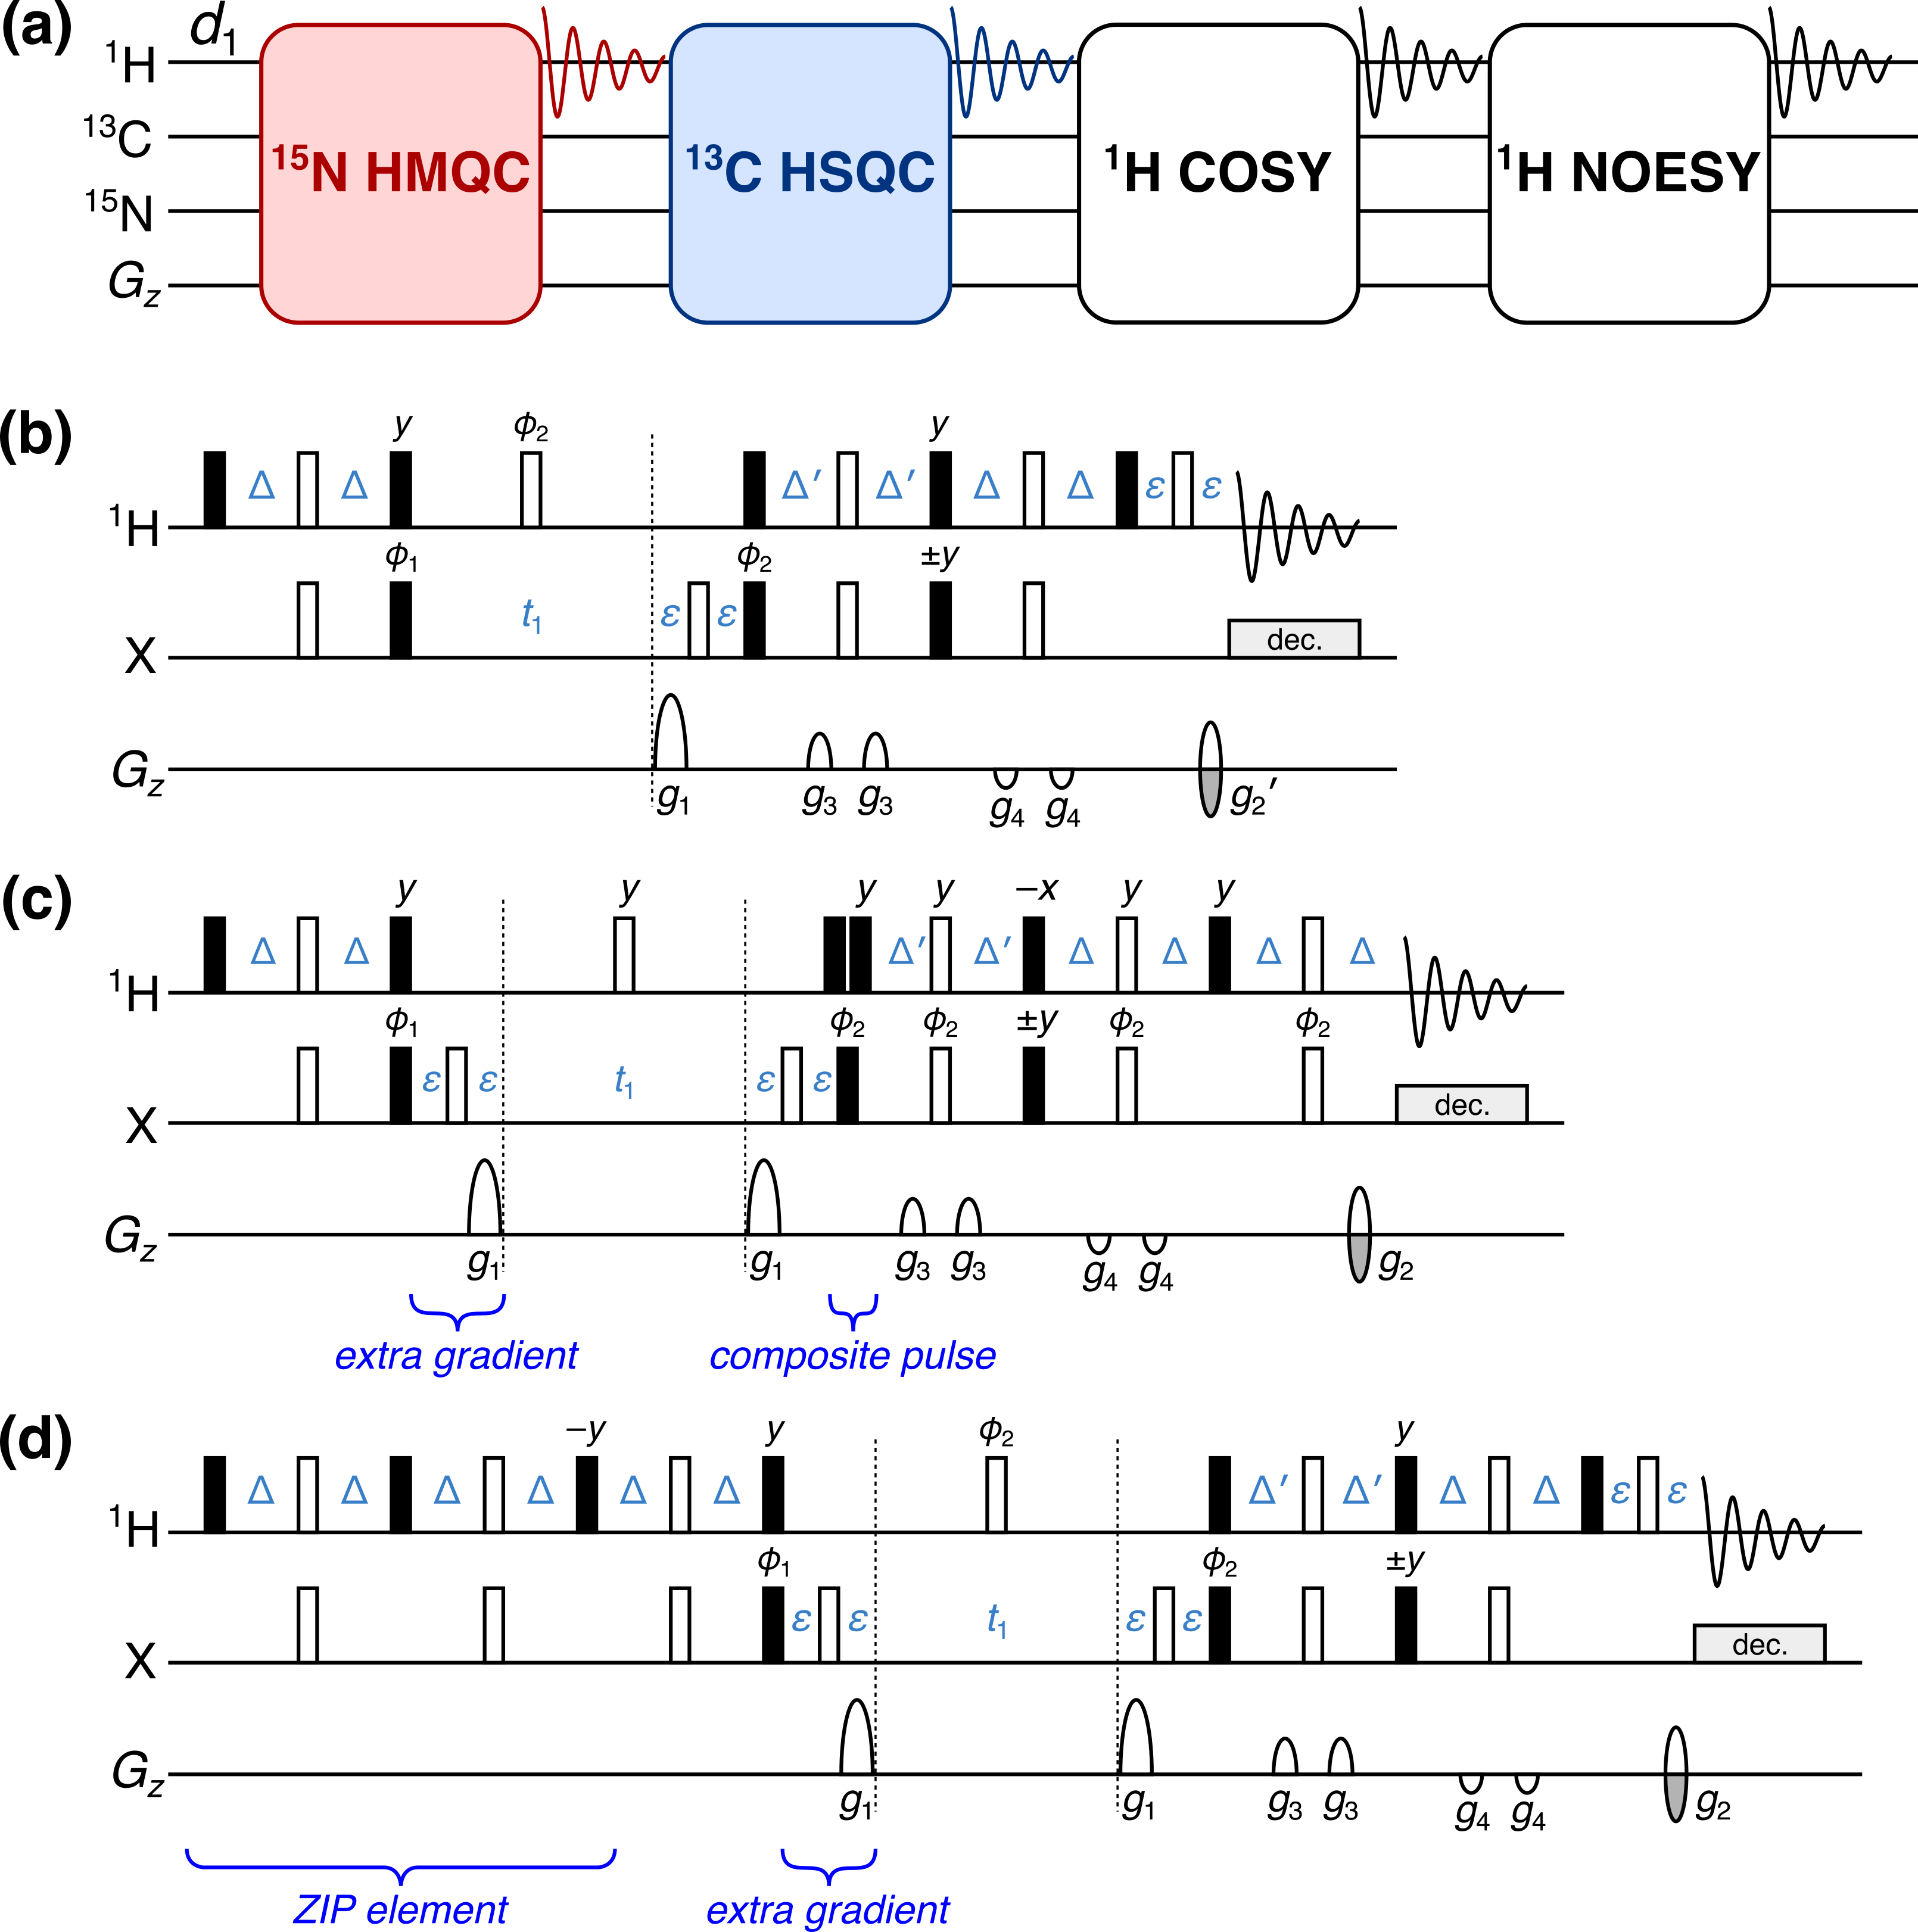
\includegraphics[width=0.7\textwidth]{pprogs.png}
    \caption{
        \textbf{(a)} Overview of a typical NOAH supersequence (MSCN, using the single-letter abbreviations previously defined\autocite{Kupce2017ACIE}).
        The \nitrogen{}--\proton{} HMQC and \carbon{}--\proton{} HSQC modules are highlighted: these may be replaced with the new seHSQC module proposed in this work.
        \textbf{(b)} Original NOAH HMQC module,\autocite{Kupce2017ACIE, Kupce2007MRC} abbreviated as ``M''.
        \textbf{(c)} Original NOAH HSQC module without sensitivity enhancement,\autocite{Kupce2017ACIE, Schulze-Sunninghausen2017JMR} abbreviated as ``S''.
        \textbf{(d)} Cavanagh--Rance--Kay (CRK) seHSQC.\autocite{sehsqc}
        \textbf{(e)} NOAH seHSQC module, abbreviated as ``Sp'' (this work).
        Filled and unfilled bars represent \ang{90} and \ang{180} pulses respectively; all \ang{180} pulses on \carbon{} are adiabatic (swept-frequency) pulses.
        All pulses are applied along $+x$ unless otherwise noted.
        The delays are chosen as follows: $\Delta = 1/(4\cdot\onejxh)$, $\Delta' = 1/(8\cdot\onejch)$ or $1/(4\cdot\onejnh)$, and $\varepsilon$ is the minimum time needed for a gradient and subsequent recovery.
        All gradients are \SI{1}{\ms} long, except for $g_1$ and $g_2$ in \nitrogen{} experiments which are \SI{2.5}{\ms} long.
        Gradient amplitudes, as percentages of maximum gradient strength, are as follows: $g_1 = 80\%$; $g_2 = \pm 40.2\%$ (\carbon{}) or $\pm 16.2\%$ (\nitrogen{}); ${g_2}' = g_2/2$; $g_3 = 11\%$; $g_4 = -5\%$.
        The signs of $g_2$ and ${g_2}'$ are alternated in each $t_1$ increment to provide echo--antiecho selection.
        Refer to \figref{pprogs_prodop} for product operator analysis.
    }
    \label{fig:pprogs}
\end{figure}

The NOAH-4 MSCN experiment (\figref{pprogs}a) is an example of a NOAH supersequence, which yields \nitrogen{} H\textbf{M}QC, \carbon{} H\textbf{S}QC, \textbf{C}OSY, and \textbf{N}OESY spectra in one single experiment.
The implementation of this supersequence relies on the fact that the output of any one module contains all the necessary magnetisation components required for downstream modules.
For example, both the standard NOAH HMQC (\figref{pprogs}b) and HSQC (\figref{pprogs}c) modules return the bulk magnetisation back to its equilibrium position ($+z$).
In the MSCN sequence, this bulk magnetisation can therefore be used as the input to the COSY and NOESY homonuclear modules which follow.
However, the original Cavanagh--Rance--Kay (CRK) seHSQC (\figref{pprogs}d) does not obey this principle: it causes bulk magnetisation to be dephased by coherence transfer pathway (CTP) gradients.
Consequently, downstream modules can only utilise any bulk magnetisation that has relaxed during the HSQC FID acquisition, leading to drastic losses in signal intensity.
This is illustrated using a NOAH-2 SpCc (seHSQC + CLIP-COSY\autocite{Koos2016ACIE}) supersequence (\figref{spor_spv2}a): while the CRK seHSQC implementation afford significant sensitivity gains (primarily for CH peaks, as predicted by theory\autocite{sehsqc_sens}), the COSY module which follows suffers from an almost complete loss of intensity.

\begin{figure}
    \centering
    % figures/spor_spv2_comp.py
    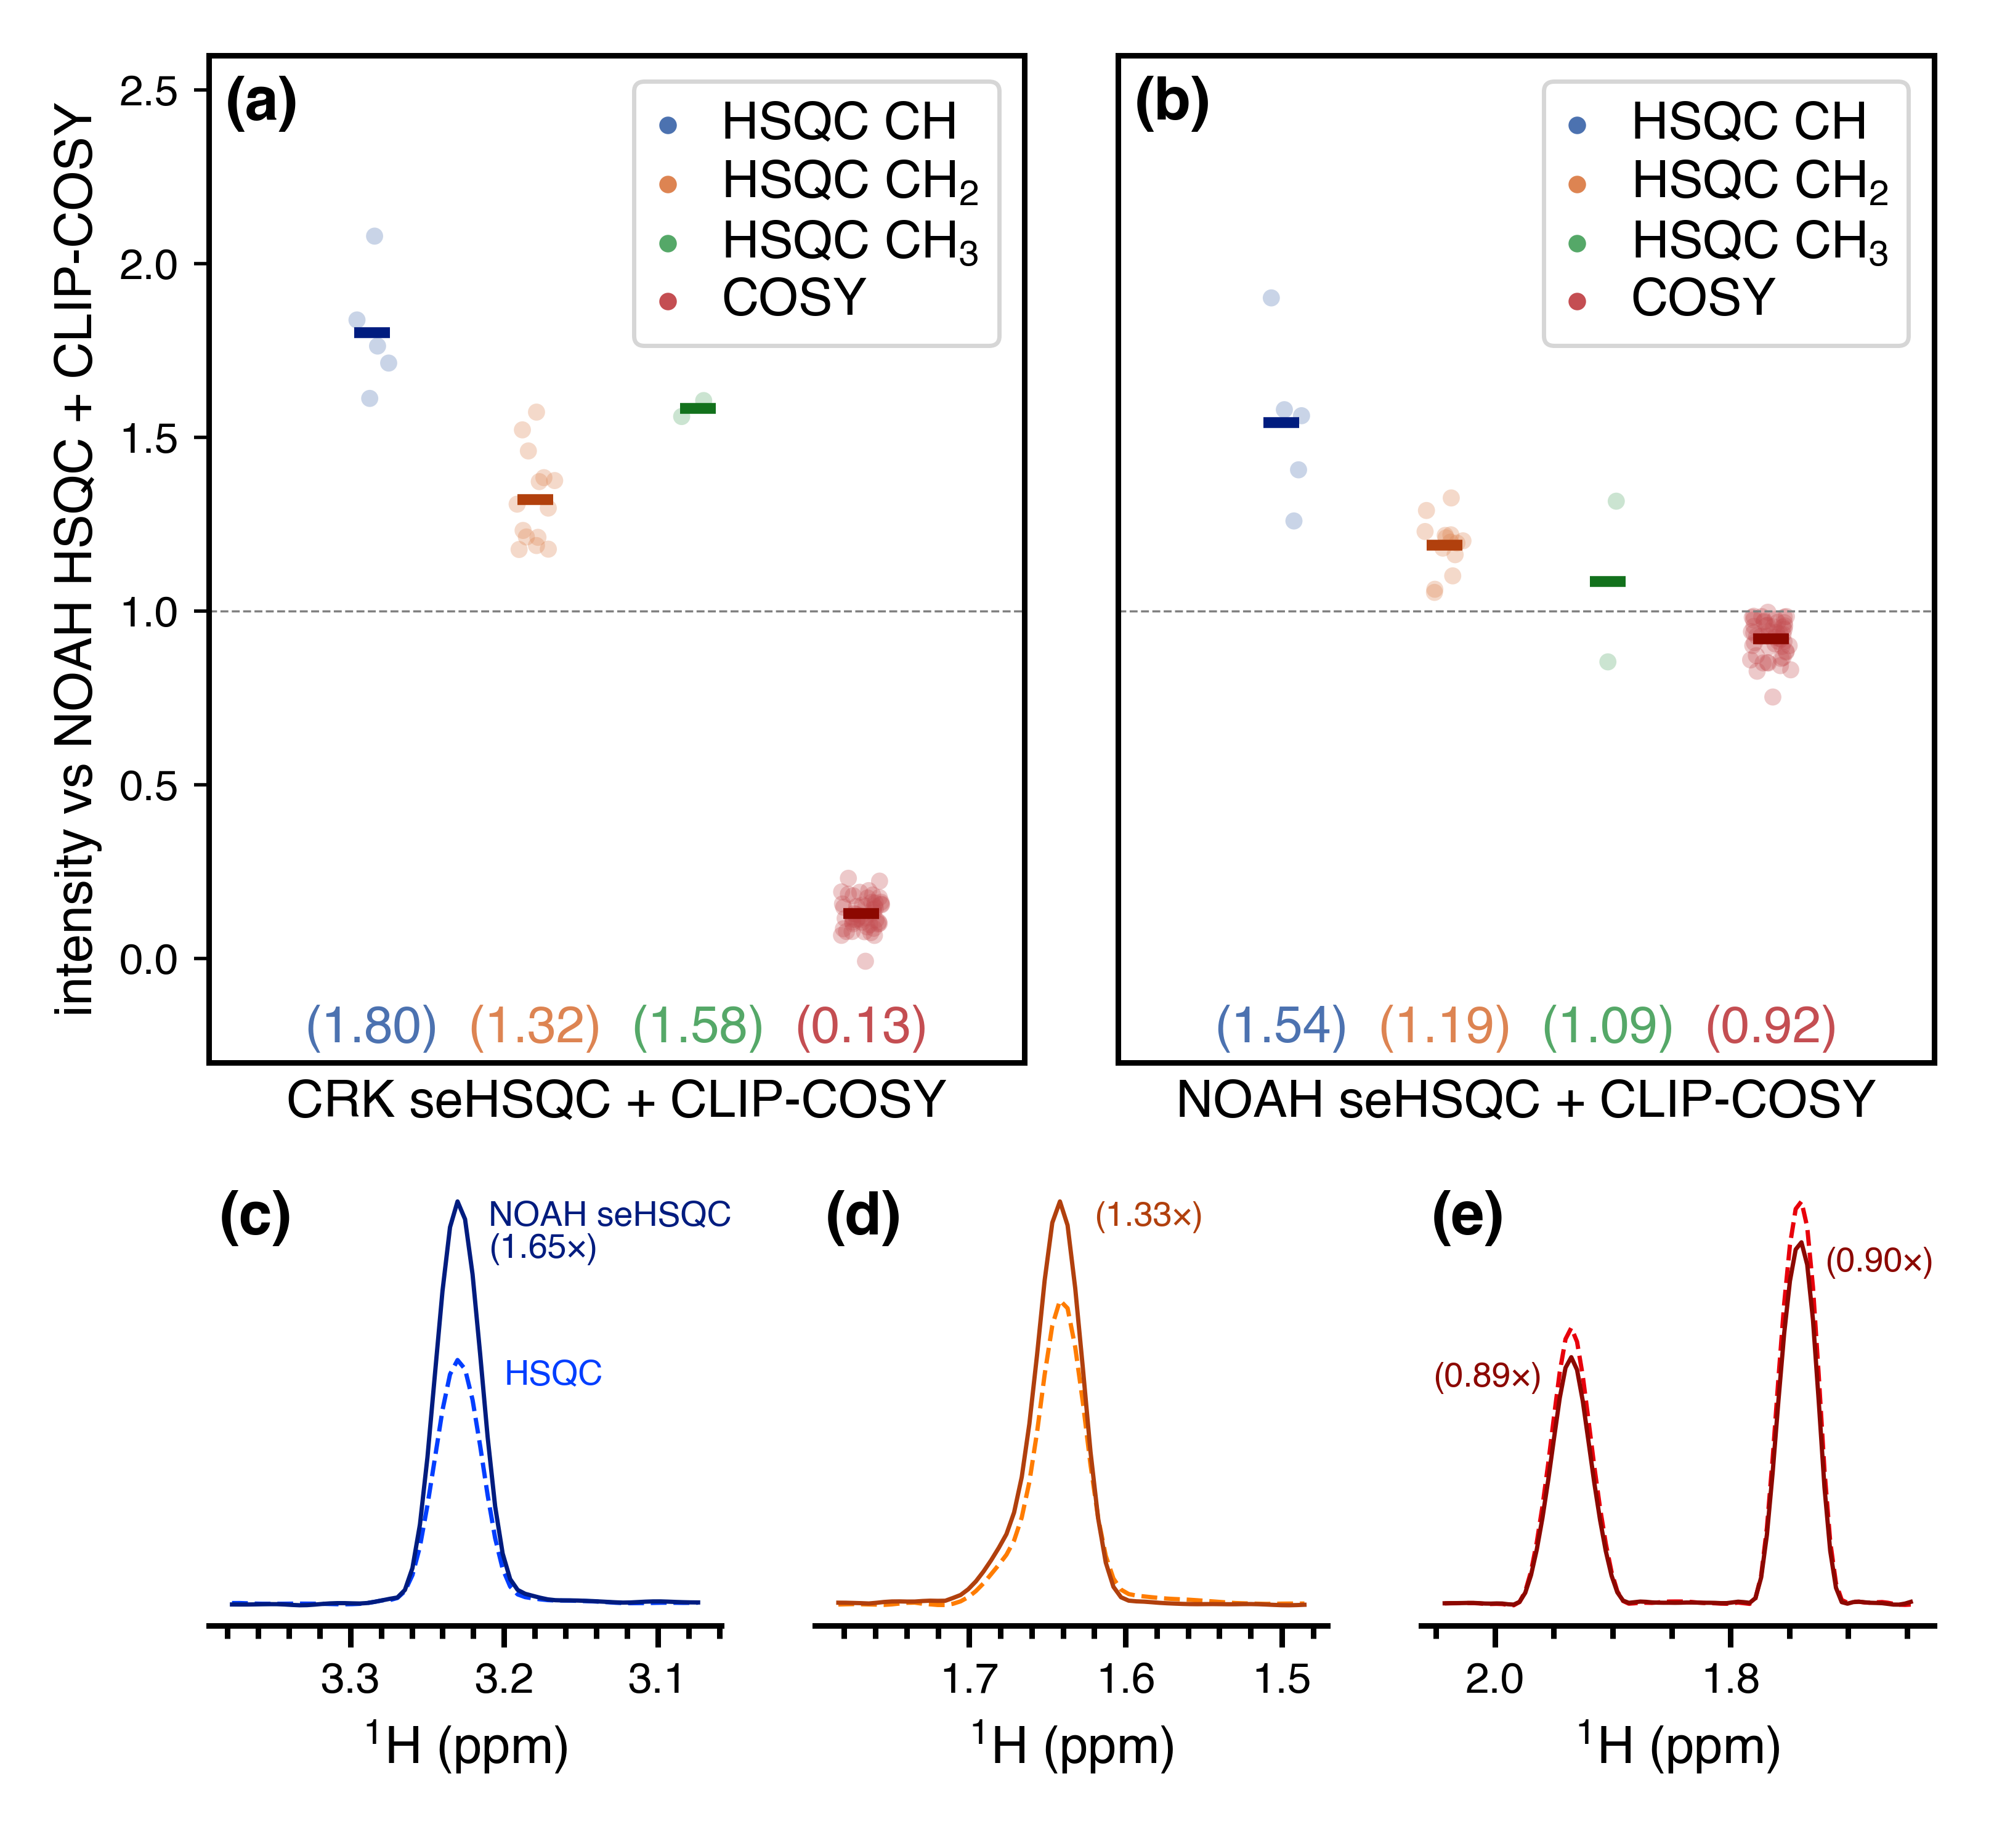
\includegraphics[width=0.6\textwidth]{spor_spv2_comp.png}
    \caption{
        \hl{We could add spectra here? I think the graph is the most important piece of information, but I'm sure people like to see spectra more than graphs...}
        Sensitivity comparisons for NOAH-2 SpCc (seHSQC + CLIP-COSY) supersequences, using the CRK (\figref{pprogs}d) and NOAH (\figref{pprogs}e) seHSQC implementations.
        All intensities are normalised against the NOAH-2 SCc (HSQC + CLIP-COSY) supersequence, without HSQC sensitivity enhancement.
        HSQC intensities are further grouped by multiplicity.
        Numbers in parentheses indicate averages over all peaks of a given type.
        \textbf{(a)} Using the original CRK seHSQC.
        The CRK seHSQC does not preserve the bulk magnetisation, leading to severely reduced COSY intensities.
        \textbf{(b)} Using the NOAH seHSQC.
        \andro{}
    }
    \label{fig:spor_spv2}
\end{figure}

Our solution is based on the simple observation that the bulk magnetisation in the seHSQC will be returned to $+z$ if the phase of the initial \proton{} \ang{90} pulse is changed by \ang{90} to $+y$.
To generate the HSQC signal, however, the same pulse needs to be applied along $+x$.
Overall, what is required is therefore a pulse sequence element which simultaneously acts as a $90^\circ_x$ (or $90^\circ_{-x})$ pulse on protons coupled to \carbon{}, and as a $90^\circ_y$ pulse on uncoupled protons.
We accomplish this by prepending a double heteronuclear spin echo, which we refer to as the \textit{isotope-specific rotation} (ISR), to the pulse sequence.
It is similar to the $zz$-filter, which we have previously used in the NOAH HMBC module to retain the magnetisation of directly coupled protons for a subsequent HSQC module.\autocite{Kupce2018CC, Kupce2019JMR}
However, the ISR has different pulse phases to this and consequently leads to a different overall outcome.
While the BIG-BIRD element developed by Briand and S{\o}rensen\autocite{Briand1997JMR} is also capable of effecting this, we find that the ISR provides greater signal-to-noise in both the seHSQC itself, as well as downstream modules (\figref{bigbird}).

In addition to the ISR, the NOAH seHSQC module also contains a CTP gradient prior to the $t_1$ period (highlighted in \figref{pprogs}e).
This gradient is not necessary for the seHSQC module itself, but instead serves to suppress artefacts in downstream modules, which would otherwise arise from bulk magnetisation that evolves during either half of the HSQC $t_1$ period.
This then evolves again in the $t_1$ period of a later homonuclear module (e.g.\ COSY), resulting in each COSY peak with $\Omega_1 = \Omega_{\ce{H}}$ being accompanied by a pair of ``wing'' artefacts at $\Omega_1 = \Omega_{\ce{H}} \pm (\Omega_{\ce{H}}\cdot\mathrm{SW}_{\ce{C}})/(2\cdot \mathrm{SW}_{\ce{H}})$, which can reach $\sim 5\%$ of the intensity of their parent peaks.
Importantly, the artefacts arising from diagonal peaks can have intensities that are comparable to genuine crosspeaks (\figref{wing_artefacts}), which highlights the importance of suppressing these artefacts.

With these modifications, the NOAH seHSQC module provides clear sensitivity gains over the NOAH HSQC module, while preserving essentially the same amount of \proton{} magnetisation for downstream modules (\figref{spor_spv2}b).
The modifications present in the NOAH seHSQC, particularly the ISR, mean that the sensitivity improvements are slightly lower as compared to the original CRK implementation.
On average, \ce{CH} and \ce{CH2} peaks have $1.54\times$ and $1.19\times$ increased sensitivity respectively relative to the NOAH HSQC module.
However, a dramatic improvement is seen in the COSY module which follows.
In contrast to the CRK seHSQC, which completely destroys the requisite bulk magnetisation, the NOAH seHSQC preserves the majority of it, performing 92\% as well as the original HSQC module.

Multiplicity editing can be easily incorporated into the NOAH seHSQC sequence (\figref{edited_sehsqc_pprog}), leading to similar sensitivity gains relative to the HSQC module.
It is noteworthy that the original NOAH HSQC (without sensitivity enhancement) places the bulk magnetisation in the $xy$-plane during the $t_1$ and editing periods, whereas the newly proposed NOAH seHSQC places the bulk along $\pm z$.
In the former, the bulk magnetisation is therefore subject to homonuclear coupling ($\jhh$) evolution, leading to a small decrease in the sensitivity of later homonuclear modules when multiplicity editing is introduced.
Since homonuclear experiments typically have a greater inherent sensitivity than the HSQC, this minor loss is not a problem, and is far outweighed by the benefits of incorporating multiplicity editing in the HSQC.
Nevertheless, the fact that the seHSQC does not suffer from such a penalty is a welcome benefit.
As a result, the edited NOAH seHSQC slightly outperforms the edited HSQC in terms of preserving bulk magnetisation, with subsequent homonuclear modules enjoying a slight boost in sensitivity (\figref{edited_sn_comp}).

\hl{On second thoughts, I'm wondering if it may not be useful to put ASAP-seHSQC stuff here...
    Firstly it's a slightly different context and I think there are considerations in ASAP that don't make much sense here -- for example use of URPs which helps to clean ASAP spectra up quite a bit but don't see much use here.
    Secondly -- especially given the recent interest in fast-repetition sequences -- there might be potential for some of that to be reported elsewhere.
    We would have to try to make a bit more sense out of various issues first though, such as how useful exactly is mixing vs relaxation, etc...}


\section*{\texorpdfstring{\nitrogen{}}{15N} seHSQC}

The proposed seHSQC module can be similarly implemented for \nitrogen{} experiments.
Currently, in NOAH supersequences, \nitrogen{}--\proton{} correlations are primarily obtained using the HMQC module, since this manipulates bulk magnetisation more favourably than the HSQC (\textit{vide infra}).\autocite{Kupce2007MRC, Kupce2017ACIE}
Compared to this, the new seHSQC module can provide greater than $4\times$ greater sensitivity (\figref{n15}).
This arises partly because of the use of the PEP sensitivity enhancement scheme, in which the \hl{reverse?} INEPT transfer delays $\Delta'$ can optimised for \ce{NH} peaks.
However, there is also a significant improvement due to the fact that peaks in the \nitrogen{} seHSQC are not broadened in the indirect dimension by $\jhh$, unlike in the HMQC.
Although the seHSQC retains a slightly smaller amount of bulk magnetisation ($\sim 70\%$, versus $\sim 80\%$ for the HMQC), this is generally not a problem, since it is the \nitrogen{} module which typically has the lowest intrinsic sensitivity in a supersequence.

\begin{figure}
    \centering
    % figures/15n_spv2vsm.py
    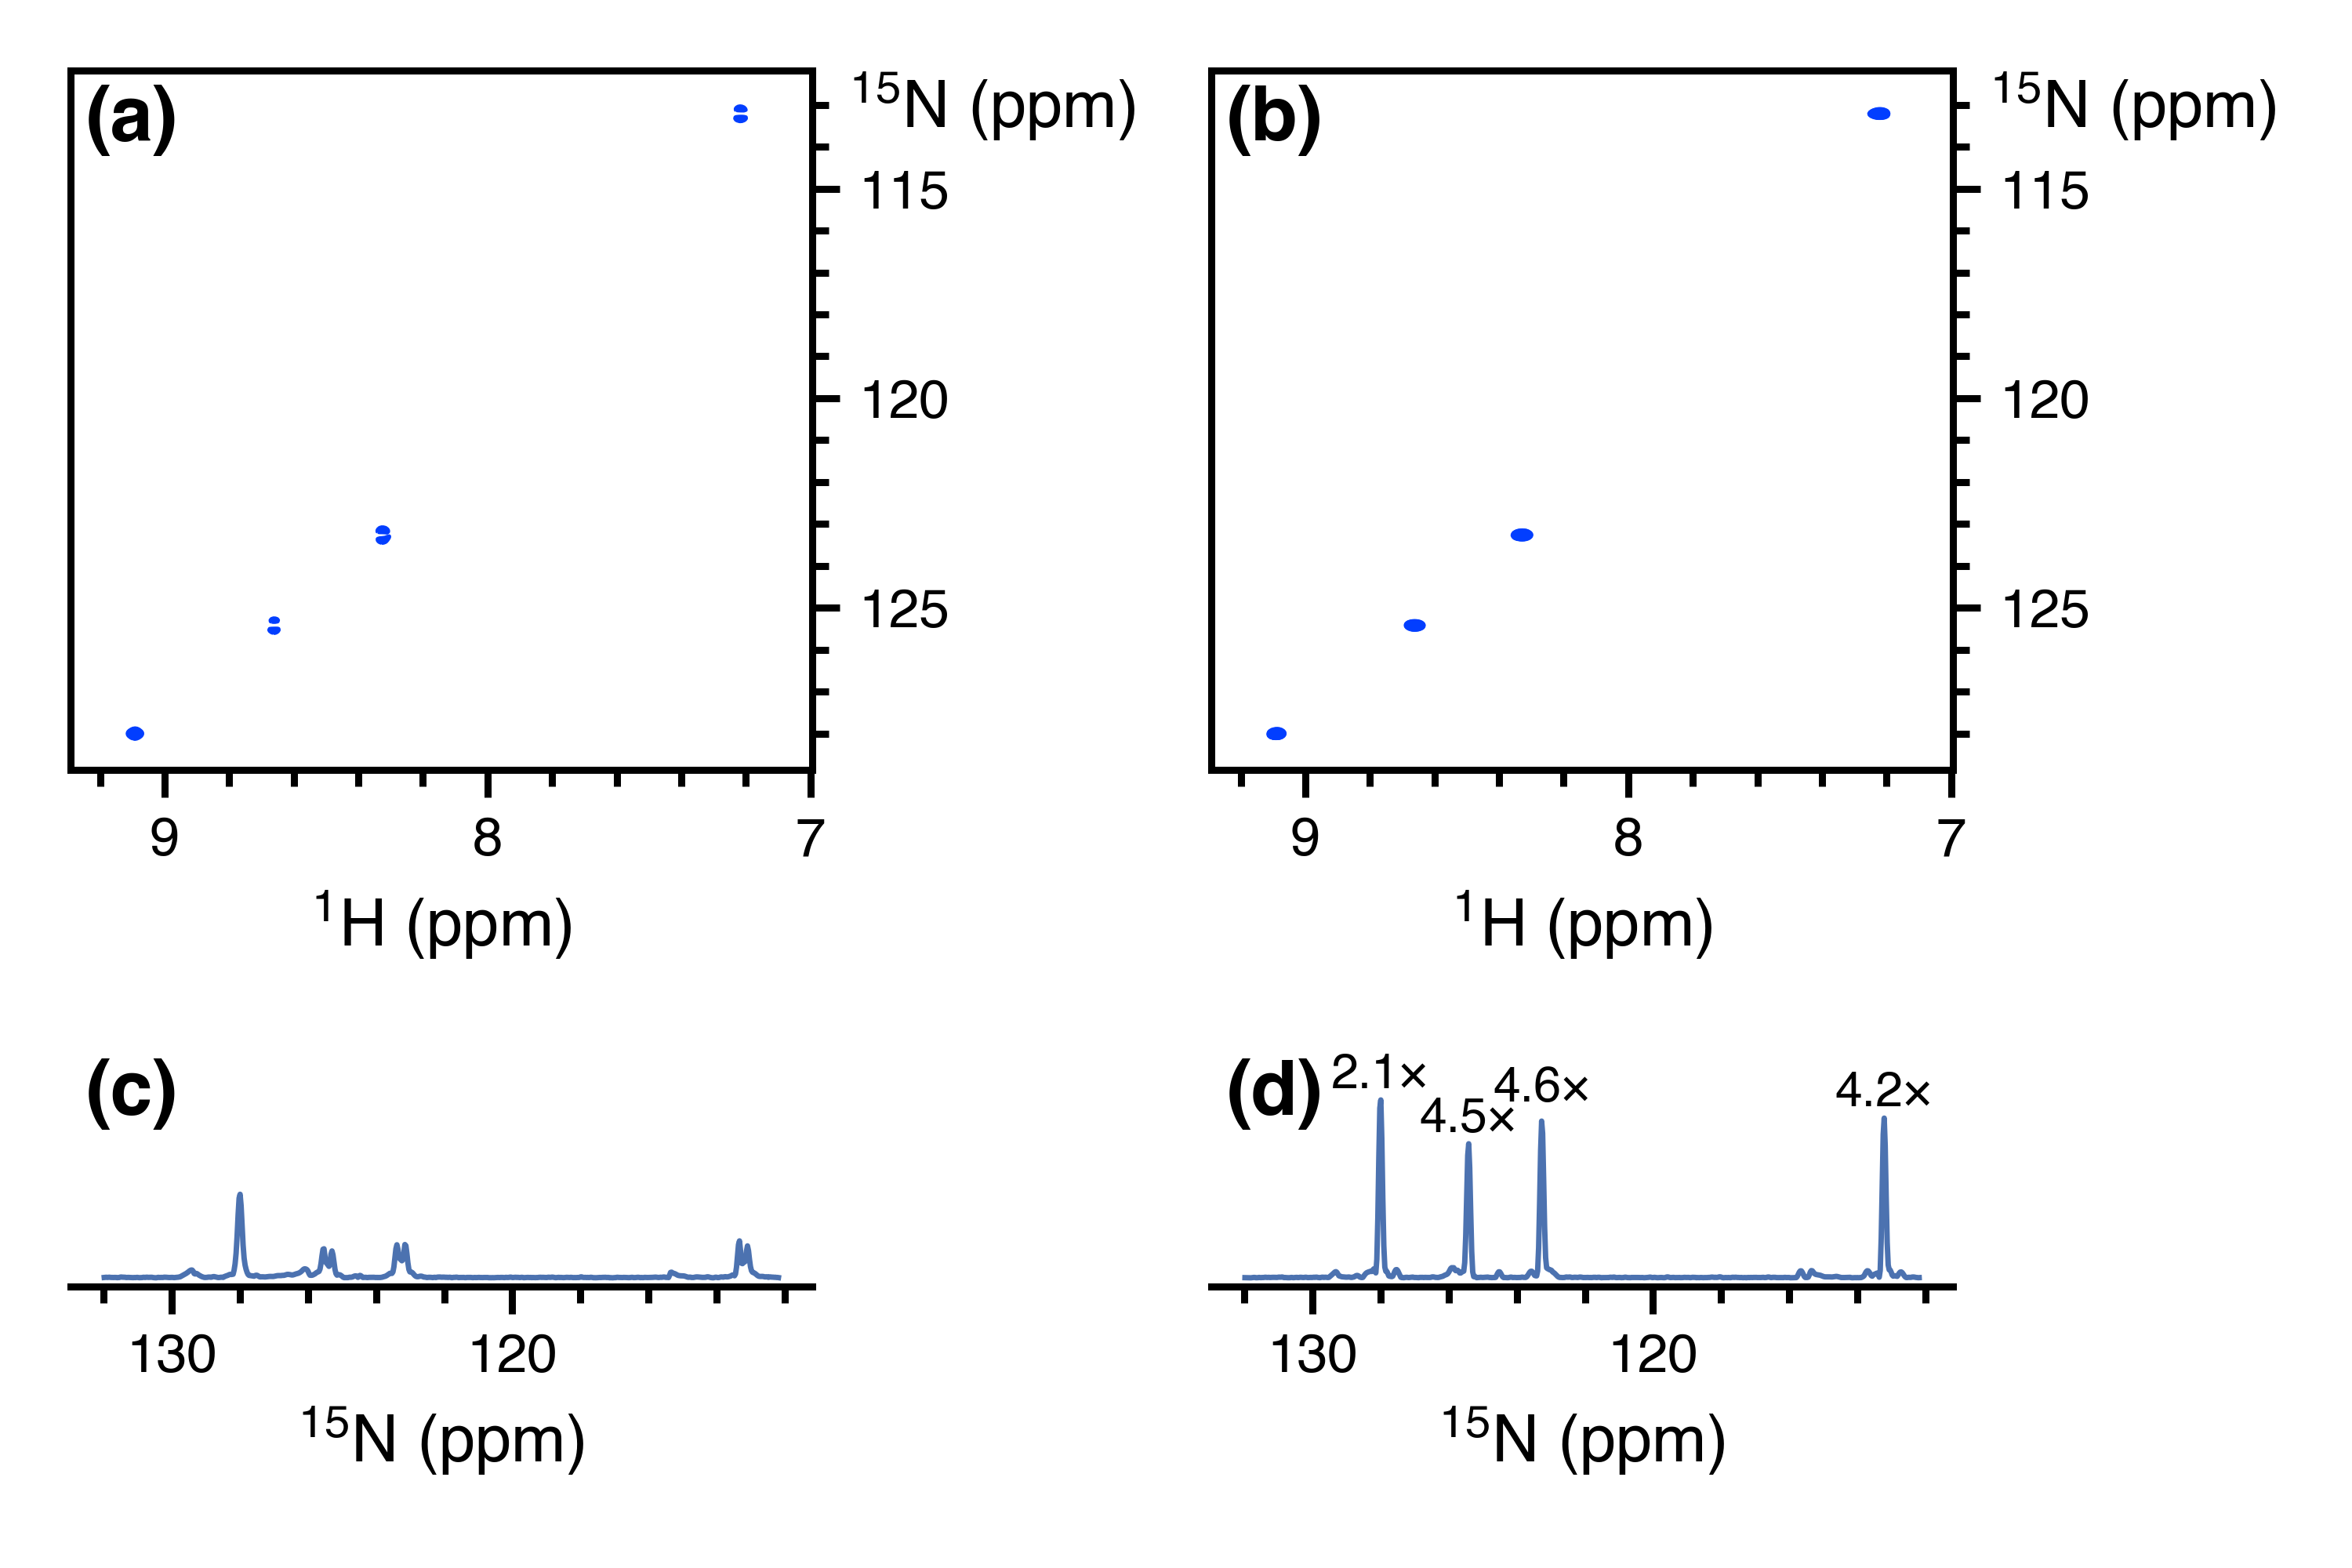
\includegraphics[width=0.6\textwidth]{15n_spv2vsm.png}
    \caption{
        Comparison of the new \nitrogen{}--\proton{} seHSQC with the standard NOAH HMQC module\hl{, taken from NOAH-3 XSpCc supersequences (\nitrogen{} experiment + \carbon{} seHSQC + CLIP-COSY)}.
        \textbf{(a)} \nitrogen{} HMQC spectrum.
        \textbf{(b)} \nitrogen{} seHSQC spectrum.
        \textbf{(c)} Projection of HMQC onto the $f_1$ axis.
        Splitting due to $\jhh$ is clearly visible for three of the four peaks.
        \textbf{(d)} Projection of seHSQC onto the $f_1$ axis.
        Signal-to-noise improvements relative to the HMQC spectrum are indicated over each peak.
        The largest gains are observed for peaks where the multiplet structure is collapsed; however, even in the absence of that, a $\sim 2\times$ gain is still obtained.
        \grami{}
    }
    \label{fig:n15}
\end{figure}

While a \nitrogen{} HSQC module (without sensitivity enhancement) would still benefit from multiplet collapse, it comes with other severe drawbacks.
As previously discussed, the HSQC module places bulk magnetisation in the $xy$-plane during the $t_1$ period.
Consequently, the amount of bulk magnetisation that is retained decreases as $t_1$ is lengthened, leading to line broadening in the indirect dimensions of all downstream modules (\figref{n15_linebroadening}).
Whilst this is not a problem with the \carbon{} HSQC where typical \carbon{} indirect dimension acquisition times are relatively short, the smaller spectral widths in \nitrogen{} experiments can mean downstream modules suffer losses in both sensitivity and resolution.
The seHSQC module avoids this issue entirely, making it especially well-suited to obtaining \nitrogen{} correlations.

For optimal performance, the \nitrogen{} seHSQC module benefits from one notable change with respect to its \carbon{} counterpart, which is that the CTP gradients $g_1$ and $g_2$ (\figref{pprogs}e) are all lengthened from a typical duration of \SI{1}{\ms} to \SI{2.5}{\ms}.
This is to more effectively dephase any residual bulk magnetisation that, due to the cumulative effect of pulse imperfections, is transverse just prior to detection.
If left uncontrolled, this magnetisation can lead to significant levels of artefacts in the seHSQC module itself (\figref{cnst16_diff}).
The \carbon{} seHSQC does not need this gradient extension because of the larger amplitude of $g_2$; however, the corresponding \nitrogen{} gradient is weaker by a factor of $\gamma_{\ce{C}}/\gamma_{\ce{N}} \approx 2.5$, thus requiring a longer duration in order to produce comparable artefact attenuation.
In practice, we find that gradient durations of 2 to \SI{2.5}{\ms} provide sufficient suppression whilst not causing any appreciable difference in the intensity of the desired crosspeaks (\figref{cnst16_diff}).

In scenarios where high resolution in the \nitrogen{} dimension is not required, it can prove useful to reduce the number of $t_1$ increments and in its place increase the number of transients acquired.\autocite{Perez-Trujillo2007MRC, Parella2010CMR}
In new versions of the NOAH pulse programmes (including those provided in the \SInf{}), this feature can be enabled by specifying a factor $k$ by which to perform this scaling.
Note that the scaling is only applied to the \nitrogen{} module; all other modules are left untouched.
In our hands, setting $k = 2$ or 4 for the \nitrogen{} HMQC can lead to significant sensitivity gains \hl{(how much?)}, since $\jhh$ splitting in the indirect dimension can no longer be resolved \sitodo{}.
This point is not relevant to the seHSQC, and here $k$-scaling on its own has only a tiny effect on peak height (and signal-to-noise), since any sensitivity gained from the extra transients is offset by the broadening.
However, the later $t_1$ increments which were not acquired can be reconstructed using linear projection \hl{(cite)} to mitigate this line broadening.
The resulting spectra display sensitivity gains of up to a factor of $k$, although the fidelity of the reconstruction suffers for $k > 4$ \sitodo.

\section*{Double HSQC and HSQC-TOCSY}

\hl{Need figure}

Next, we note that the HSQC module (though not the new seHSQC module) allows an arbitrary amount of \carbon{}--\proton{} magnetisation to be excited, with the remainder returned to $+z$.  In order to excite a proportion $f$ of \carbon{}--\proton{} magnetisation ($0 < f \leq 1$), the initial INEPT delay must be shortened by a factor of $\sin^{-1}f$.
The remaining $(1 - f)$ of the magnetisation, plus any that recovers during the first HSQC FID, can then be used for a second HSQC module in the same supersequence.
The collection of multiple HSQC spectra in one multi-FID acquisition (MFA) experiment has previously been accomplished by keeping the two CTPs in the CRK seHSQC separate, with the cosine- and sine-modulated CTPs each contributing to one spectrum.\autocite{ctphsqc}
However, with a value of $f = 0.7$, the NOAH strategy already provides slightly higher sensitivity for both spectra.
Furthermore, the sensitivity of the second HSQC can be further boosted by using the new seHSQC module in place of it \sitodo{}.

By adding a period of isotropic mixing prior to detection, the NOAH HSQC module may be converted to a HSQC-TOCSY module.
This is similar to the previously reported ASAP-HSQC-TOCSY,\autocite{Becker2019JMR} the key difference being that in the present NOAH context, unused \carbon{}--\proton{} and bulk magnetisation is preserved for use in other modules, instead of later $t_1$ increments as in the ASAP experiment.
Compared to the existing MFA HSQC-TOCSY/HSQC experiment,\autocite{Nolis2019CPC} our approach displays greater flexibility in three regards.
Firstly, the vast majority of bulk magnetisation is preserved, allowing for homonuclear module(s) to be appended in a NOAH supersequence (in practice, losses of ca.\ 10\% are observed due to pulse imperfections).
On the other hand, the MFA sequence, much like the original CRK seHSQC which it is based on, dephases bulk magnetisation and causes a 80--90\% sensitivity loss in downstream spectra.
Secondly, the sensitivity of both spectra can be optimised through the value of $f$; this allows a larger amount of \carbon{}--\proton{} magnetisation to be used for the inherently less sensitive HSQC-TOCSY (in our experience, setting $f = 0.9$ provides a good balance).
In contrast, isotropic mixing in the MFA sequence is applied to the less sensitive sine-modulated component, leading to spectra with imbalanced sensitivity.
Lastly, since each NOAH module is independently executed, the NOAH approach allows multiplicity editing to be enabled for only the HSQC and not the HSQC-TOCSY, where accidental overlap may lead to crosspeaks being lost unexpectedly.

Despite these benefits, it should be noted that the NOAH HSQC-TOCSY module will still have lower overall sensitivity than a conventional seHSQC-TOCSY, which can make use of the PEP scheme.
It is not possible to simply insert a TOCSY mixing block into the seHSQC module presented here, as that will lead to the bulk magnetisation being dephased.
As usual, the benefits of fast acquisition schemes such as NOAH are most obviously realised in sufficiently concentrated samples, where NMR data acquisition times are chiefly limited by the requisite number of $t_1$ increments.
In such settings, the same amount of data can be collected in much shorter times, without worrying about the slight loss in sensitivity inherent to all fast acquisition schemes.
On the other hand, for dilute samples where this sensitivity loss is less easily tolerated, the \textit{sensitivity per unit time} of each supersequence must then be taken into consideration.
As long as the time savings outweigh any sensitivity losses, use of the NOAH supersequence will then prove to be a net benefit.
Systematic investigations in this area will be detailed elsewhere.

\hl{
    Assorted thoughts:
    \begin{enumerate}
        \item Do we need a figure illustrating the reduced delay and the HSQC-TOCSY pulse sequence? Should it be merged with the existing Fig 1, or Fig 4?
        \item I hope I have not been too critical of Parella's work. Everything I wrote \textit{is} true, and I want to say something positive about our work, but when that's the only real basis for comparison I feel like I might be being a bit harsh!
    \end{enumerate}
}

\section*{Example spectra and conclusion}

\begin{figure}
    \centering
    % figures/spstspcc.py
    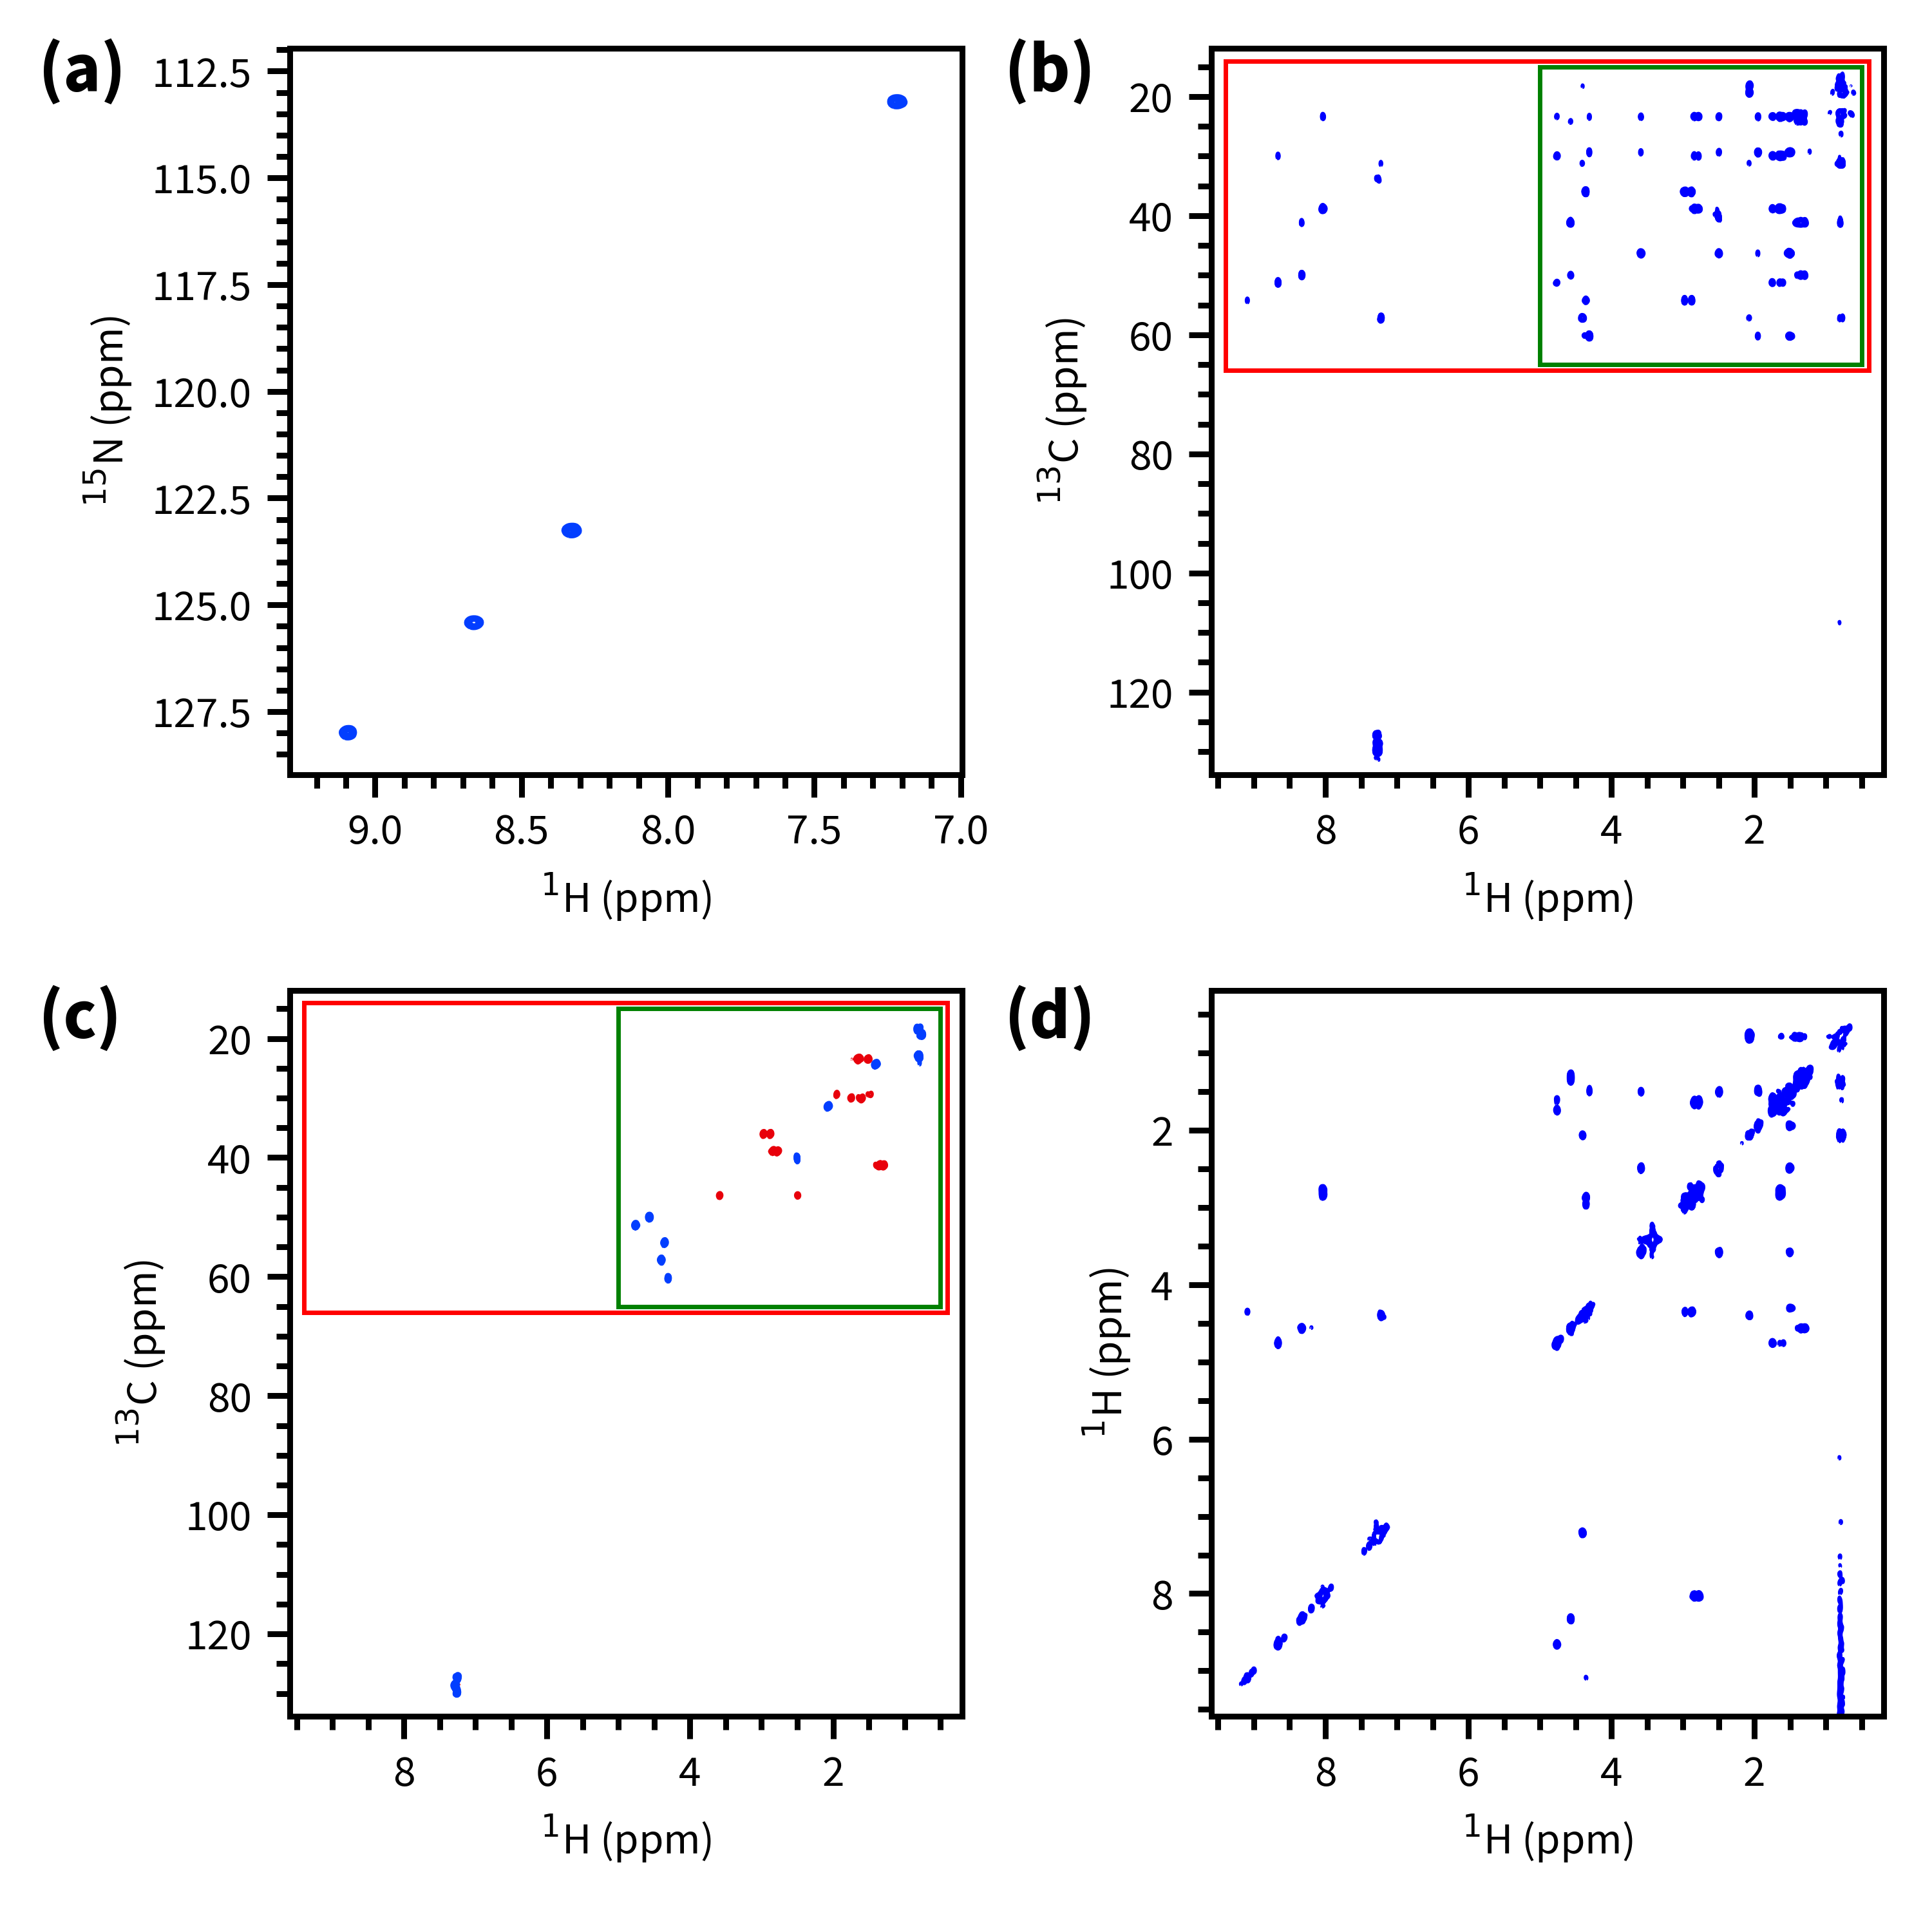
\includegraphics[width=0.6\textwidth]{spstspcc.png}
    \caption{
        Example spectra obtained from the NOAH-4 SpStSpCc supersequence.
        256 $t_1$ increments were used, with 2 scans per increment.
        The total experiment time was 17 minutes and 35 seconds.
        \textbf{(a)} \nitrogen{} seHSQC.
        \textbf{(b)} \carbon{} HSQC-TOCSY ($f = 0.9$).
        \textbf{(c)} Multiplicity-edited \carbon{} seHSQC. Notice that having the edited seHSQC removes the need for the less desirable HSQC-TOCSY editing.
        \textbf{(d)} CLIP-COSY.
        \grami{}
    }
    \label{fig:example_spec}
\end{figure}

The NOAH-4 SpStSpCc (\nitrogen{} seHSQC, \carbon{} HSQC-TOCSY, \carbon{} seHSQC, and CLIP-COSY) supersequence is one of many ways in which the new modules discussed above can be included in practical experiments.
The spectra thus obtained are shown in \figref{example_spec}.
While individual collection of the four spectra above would require 57 minutes and 8 seconds, the NOAH-4 supersequence takes only 17 minutes and 35 seconds, which represents a $3.25\times$ speedup.
One can also prepend the NOAH HMBC module;\autocite{Kupce2019JMR} this uses the semi-adiabatic $zz$-filter to preserve magnetisation of protons directly coupled to \carbon{} and \nitrogen{} heteronuclei, which is precisely the magnetisation required by the HSQC-based modules presented here.
Examples of such spectra, with time savings of up to $3.8\times$, are shown in the \SInf{} \sitodo{}.

\hl{Mention / emphasise BStSX type modules here -- applicable for typical organic molecules}

The new seHSQC and HSQC-TOCSY implementations add to the preexisting diversity in NOAH modules, bringing the total number of plausible NOAH supersequences to over 600.
The AU scripts needed for processing of these modules, as well as a number of the more commonly used pulse sequences, are provided in the \SInf{}; others are available upon request from the authors.
However, a more user-friendly and customisable method for the generation of NOAH pulse sequences is clearly needed to handle the sheer variety currently available.
Our work towards this will be reported in the near future.

\hl{
    Final assorted thoughts:
    \begin{enumerate}
        \item We should probably provide ``new'' versions of pulse programmes here. The only thing that is backwards-\textit{incompatible} is the NUS implementation. Can we introduce that in the SI? [Perhaps just to avoid confusion, we should rename the new NUS script \texttt{noah\_nus2.py}?]
    \end{enumerate}
}


\section*{Acknowledgements}

J.R.J.Y.\ thanks the Clarendon Fund (University of Oxford) and the EPSRC Centre for Doctoral Training in Synthesis for Biology and Medicine (EP/L015838/1) for a studentship, generously supported by AstraZeneca, Diamond Light Source, Defence Science and Technology Laboratory, Evotec, GlaxoSmithKline, Janssen, Novartis, Pfizer, Syngenta, Takeda, UCB, and Vertex.
\hl{Any other acknowledgements?}

% Fakesection Bibliography
\printbibliography

% Fakesection SI
% Preamble-ish commands {{{
\newcommand{\sectionbreak}{\clearpage}
\renewcommand*{\thefigure}{S\arabic{figure}}
\renewcommand*{\thetable}{S\arabic{table}}
\renewcommand*{\thepage}{S\arabic{page}}
\setcounter{page}{1}
\setcounter{figure}{0}
\setcounter{table}{0}
\onehalfspacing
% }}}
% Title page {{{
\hspace{0pt}
\vfill
\begin{center}
    \huge
    Supporting Information

    \textit{for}

    Diversifying NMR Supersequences with New HSQC-based Modules

    \vspace{1cm}

    \Large Jonathan R. J. Yong,\textsuperscript{1} \hl{[...?],} {\=E}riks Kup{\v{c}}e,\textsuperscript{2} Tim D. W. Claridge\textsuperscript{1,}*

    \vspace{1cm}

    \large \textsuperscript{1} \textit{Chemistry Research Laboratory, Department of Chemistry, University of Oxford, Mansfield Road, Oxford, OX1 3TA, U.K.}

    \textsuperscript{2} \textit{Bruker UK Ltd., Banner Lane, Coventry, CV4 9GH, U.K.}

    * \texttt{tim.claridge@chem.ox.ac.uk}
\end{center}
\thispagestyle{empty}
\vfill
\hspace{0pt}
\newpage
%}}}

% Table of contents {{{
\tableofcontents

\newpage
%}}}

\section{Product operator analysis for NOAH modules}

\begin{figure}
    \centering
    % Inkscape
    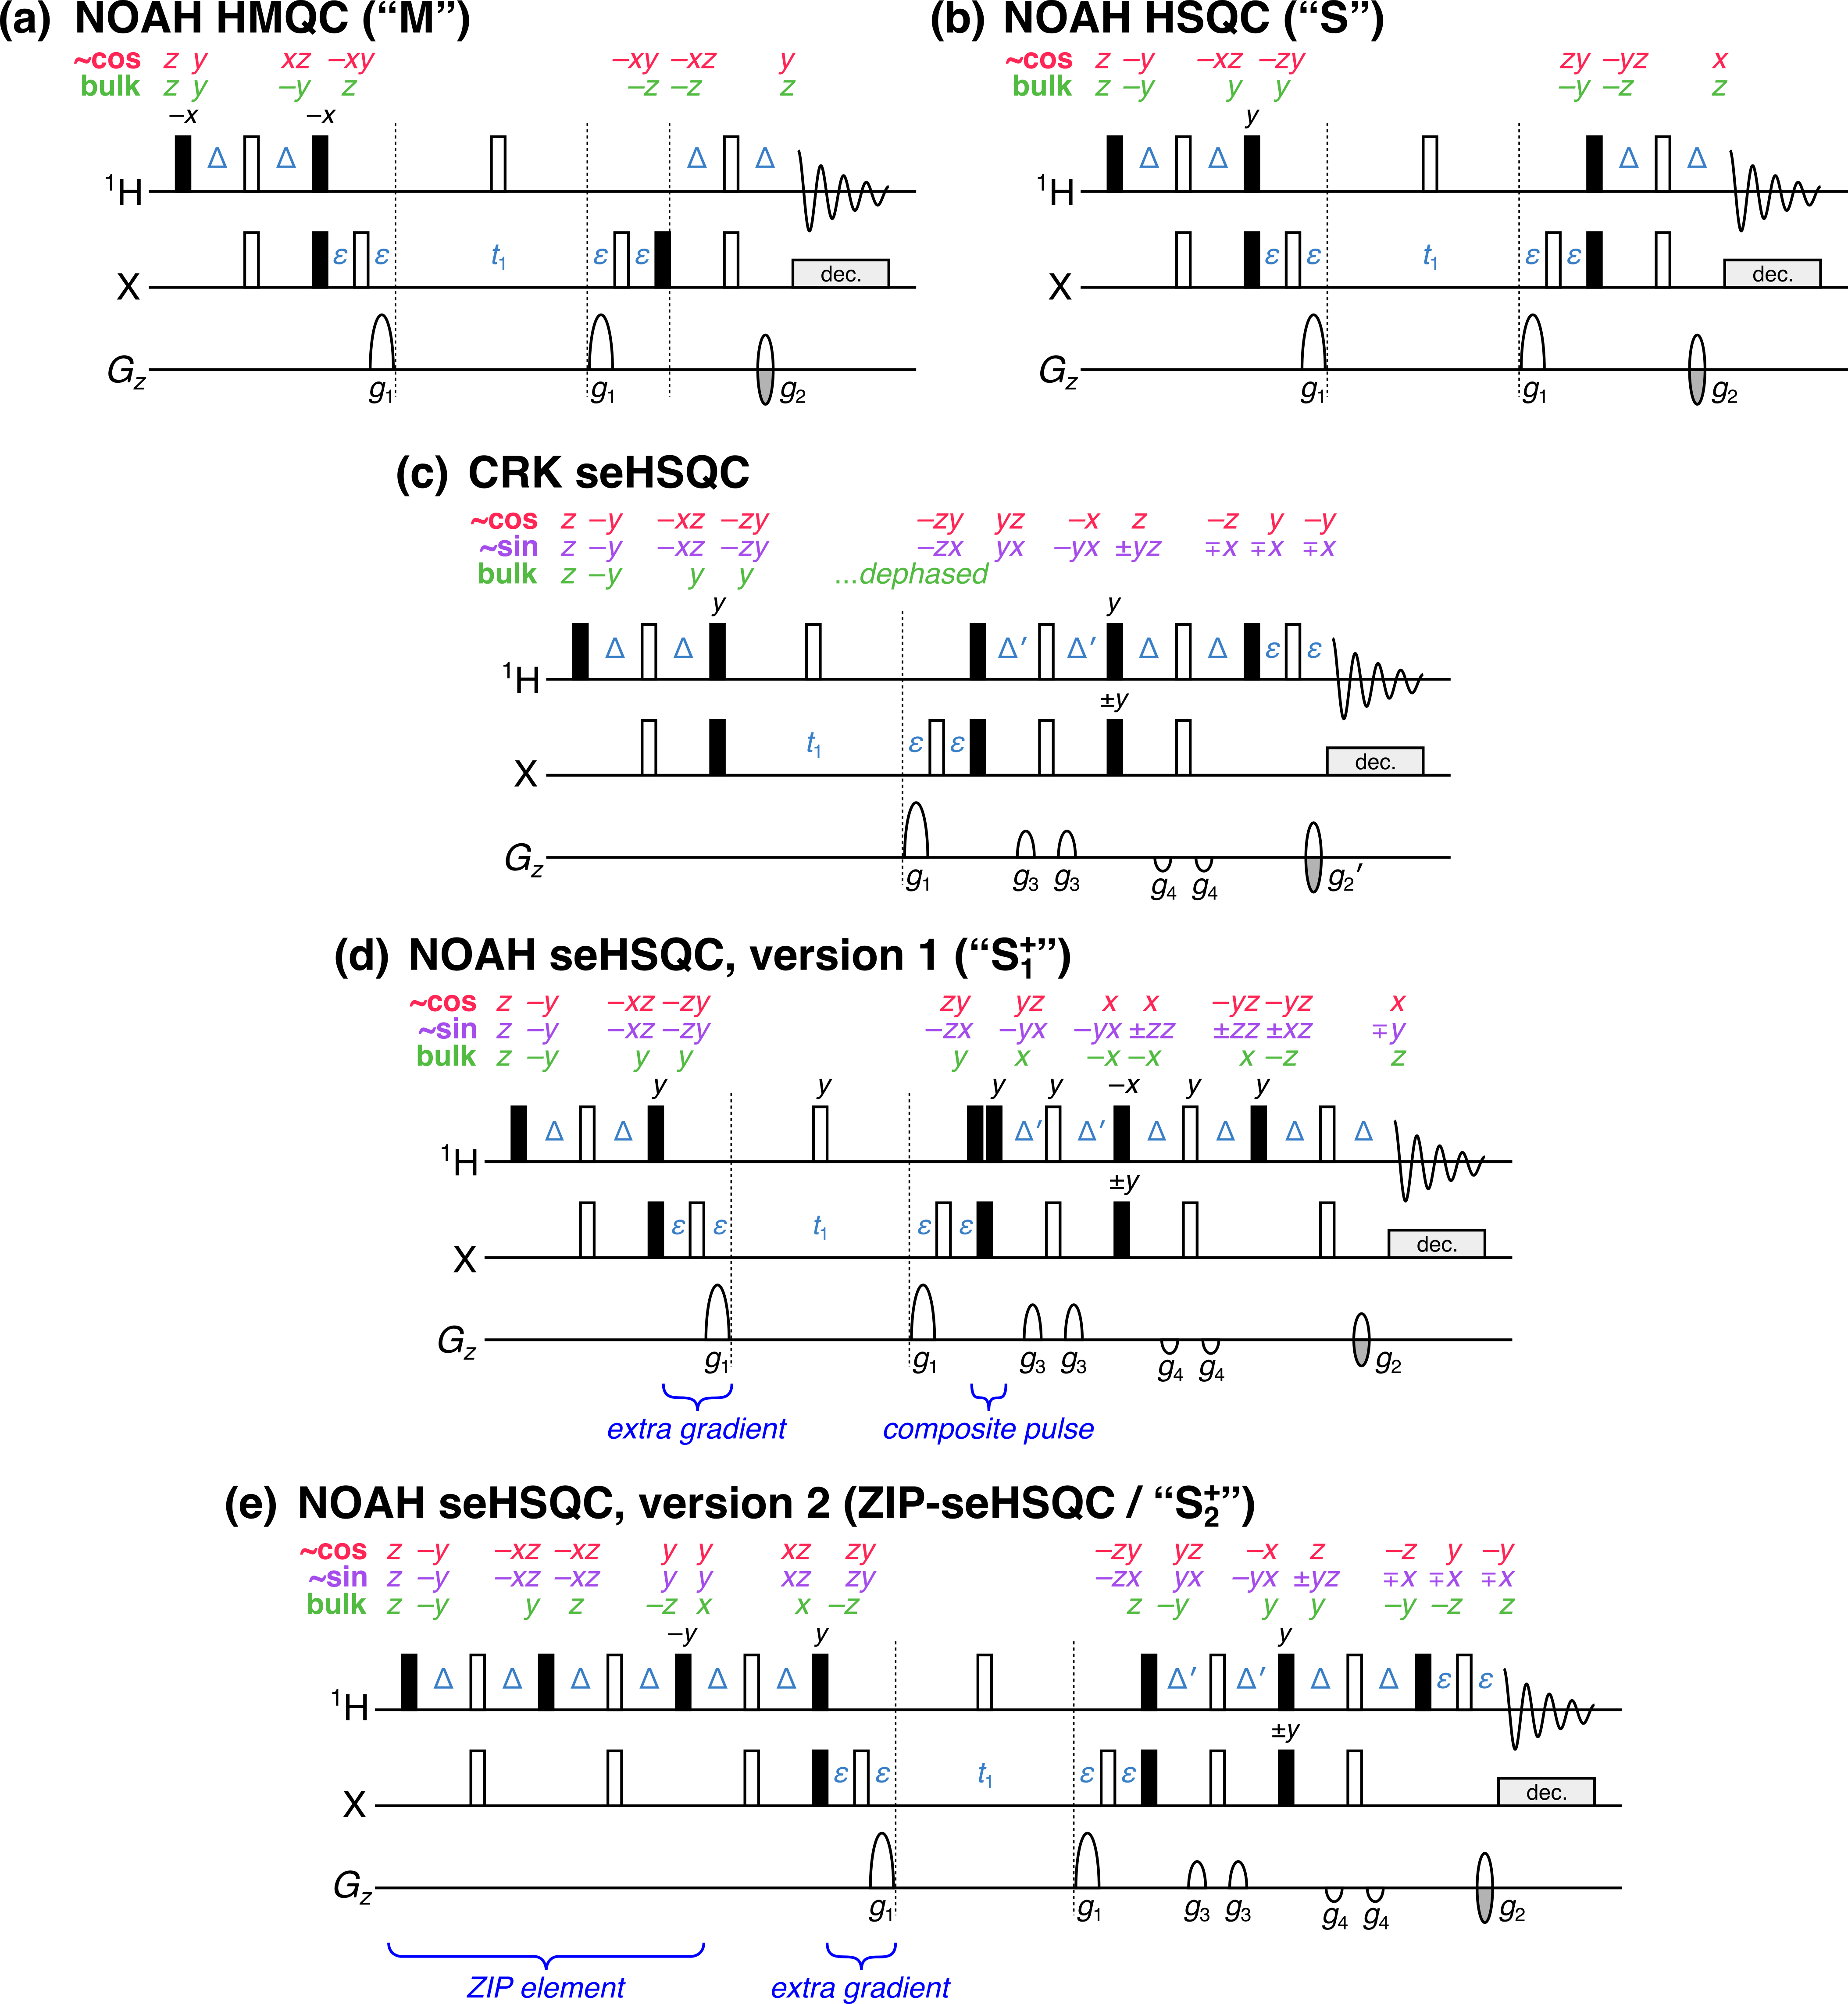
\includegraphics[width=0.8\textwidth]{./figures/pprogs_prodop.png}
    \caption{
        Product operators present at each stage of NOAH modules for an IS spin system.
        One-letter terms $m$ ($m \in \{x, y, z\}$) are shorthand for single-spin terms on proton, i.e.\ $\hat{I}_m$.
        Two-letter terms $mn$ are shorthand for two-spin terms on both the proton and heteronucleus, i.e.\ $2\hat{I}_m\hat{S}_n$.
        ``$\sim$cos'' represents the pathway for directly coupled proton magnetisation that is cosine-modulated after $t_1$: for the HMQC and HSQC, this is the only component that is detected.
        For the seHSQC, the sine-modulated component (labelled with ``$\sim$sin'') is also detected.
        ``bulk'' refers to the bulk magnetisation, i.e.\ protons that are not directly coupled to the heteronucleus.
        \textbf{(a)} NOAH HMQC.
        \textbf{(b)} NOAH HSQC.
        \textbf{(c)} NOAH seHSQC with ISR.
        Immediately following the ISR pulse sequence element, directly bonded protons are rotated onto $+y$, whereas the bulk magnetisation is rotated onto $+x$.
        Note that this analysis assumes $\Delta = \Delta' = 1/(4\cdot\onejxh)$.
    }
    \label{fig:pprogs_prodop}
\end{figure}

\section{Multiplicity editing in seHSQC}

\begin{figure}
    \centering
    % done in Inkscape
    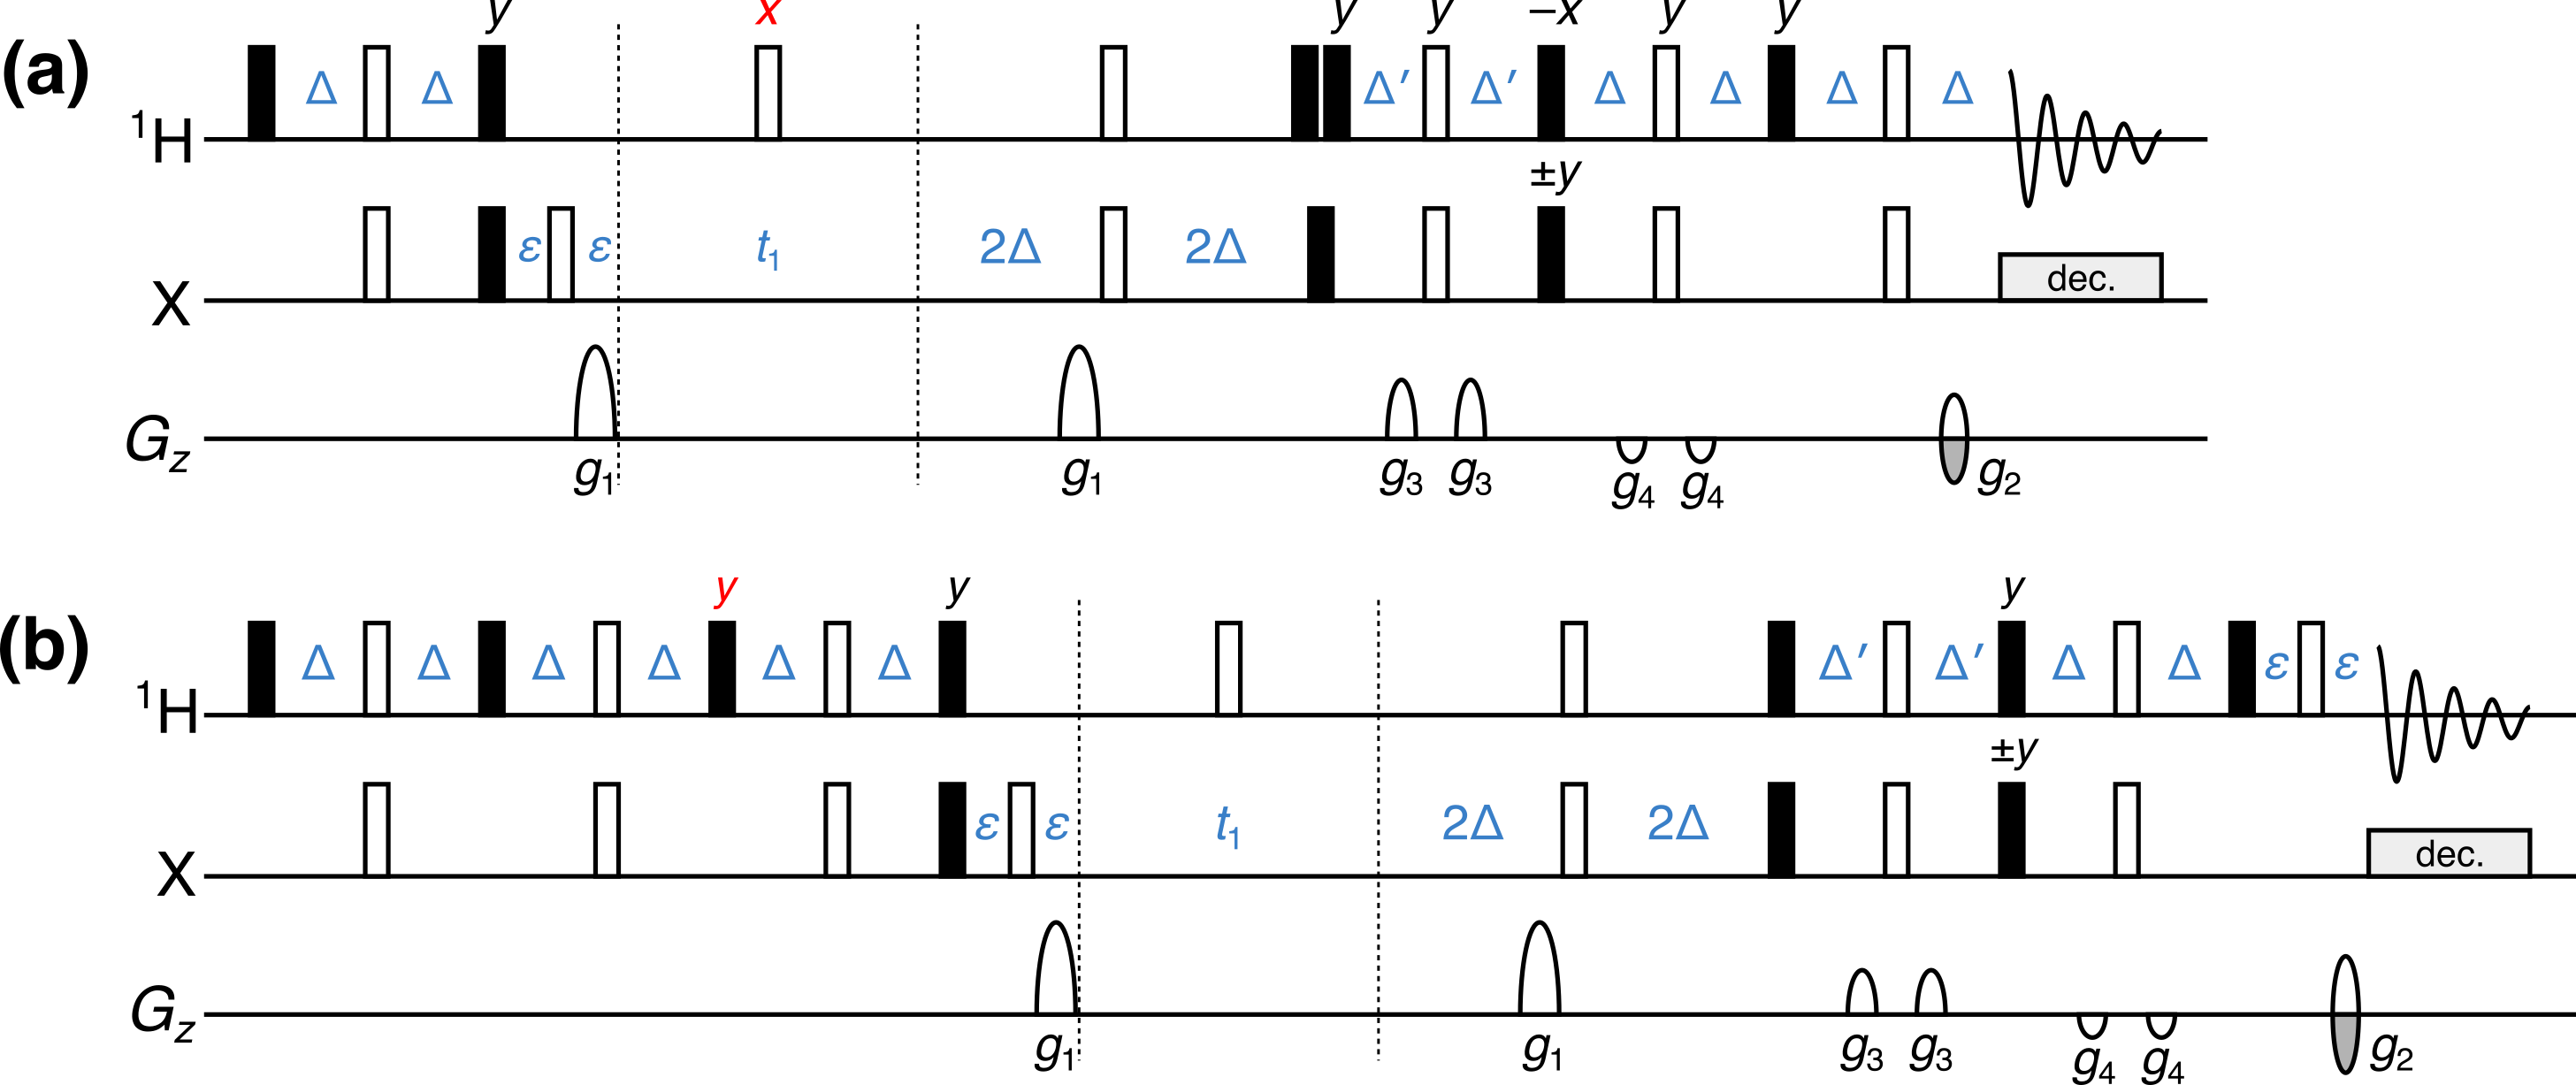
\includegraphics[width=0.8\textwidth]{./figures/mult_edit.png}
    \caption{
        Implementation of multiplicity editing in the new NOAH seHSQC module.
        Note the different phase in the third \proton{} \ang{90} pulse ($+y$ as opposed to the $-y$ in \figref{pprogs_prodop}c).
        This is needed to compensate for the extra \proton{} \ang{180} pulse in the editing period.
        Symbols have the same meaning as in \figref{pprogs} of the main text.
    }
    \label{fig:edited_sehsqc_pprog}
\end{figure}

\begin{figure}
    \centering
    % figures/edited_sn_comp.py
    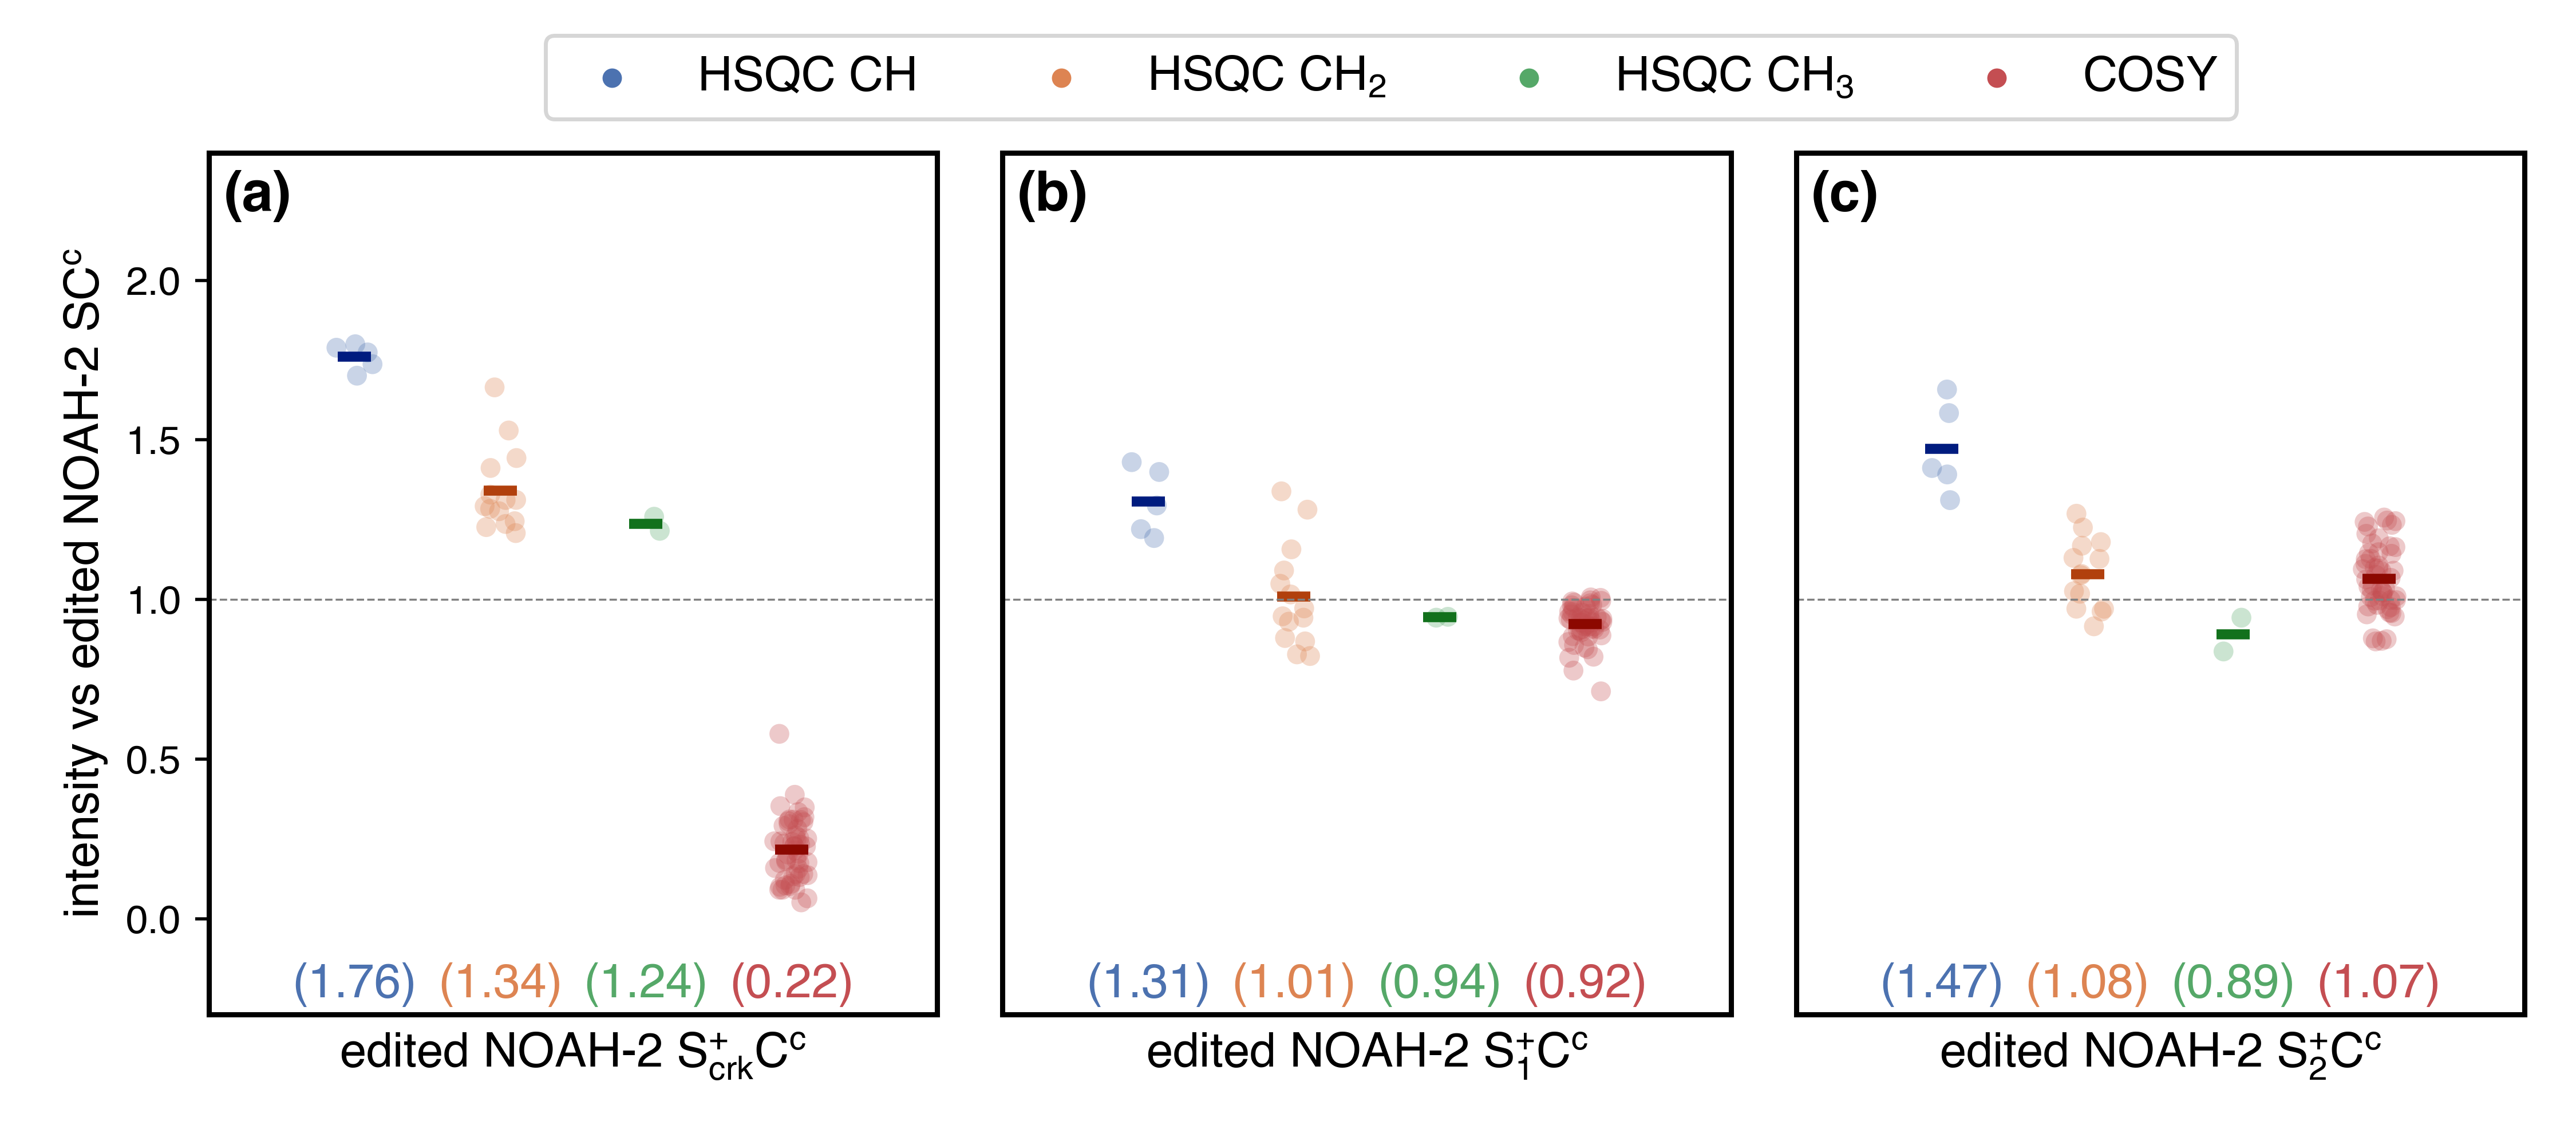
\includegraphics[width=0.8\textwidth]{./figures/edited_sn_comp.png}
    \caption{
        Sensitivity of multiplicity-edited \noahtwo{Sp}{Cc} supersequence, relative to the \noahtwo{S}{Cc} supersequence.
        Spectra were obtained with $\Delta' = 1/(8\cdot\onejch)$.
        \textbf{(a)} CRK edited seHSQC + CLIP-COSY.
        Although larger gains are observed in the HSQC, the COSY intensities are severely decreased.
        \textbf{(b)} NOAH edited seHSQC + CLIP-COSY.
        On average, sensitivity gains are observed in both the HSQC and COSY modules relative to the standard NOAH HSQC (except for HSQC \ce{CH3} peaks).
        \andro{}
    }
    \label{fig:edited_sn_comp}
\end{figure}

\section{Effect of setting \texorpdfstring{$\Delta' = 1/(4\cdot\onejch)$}{Delta' = 1/(4*1JCH)} in seHSQC}

\begin{figure}
    \centering
    % figures/combined_1_4j.py
    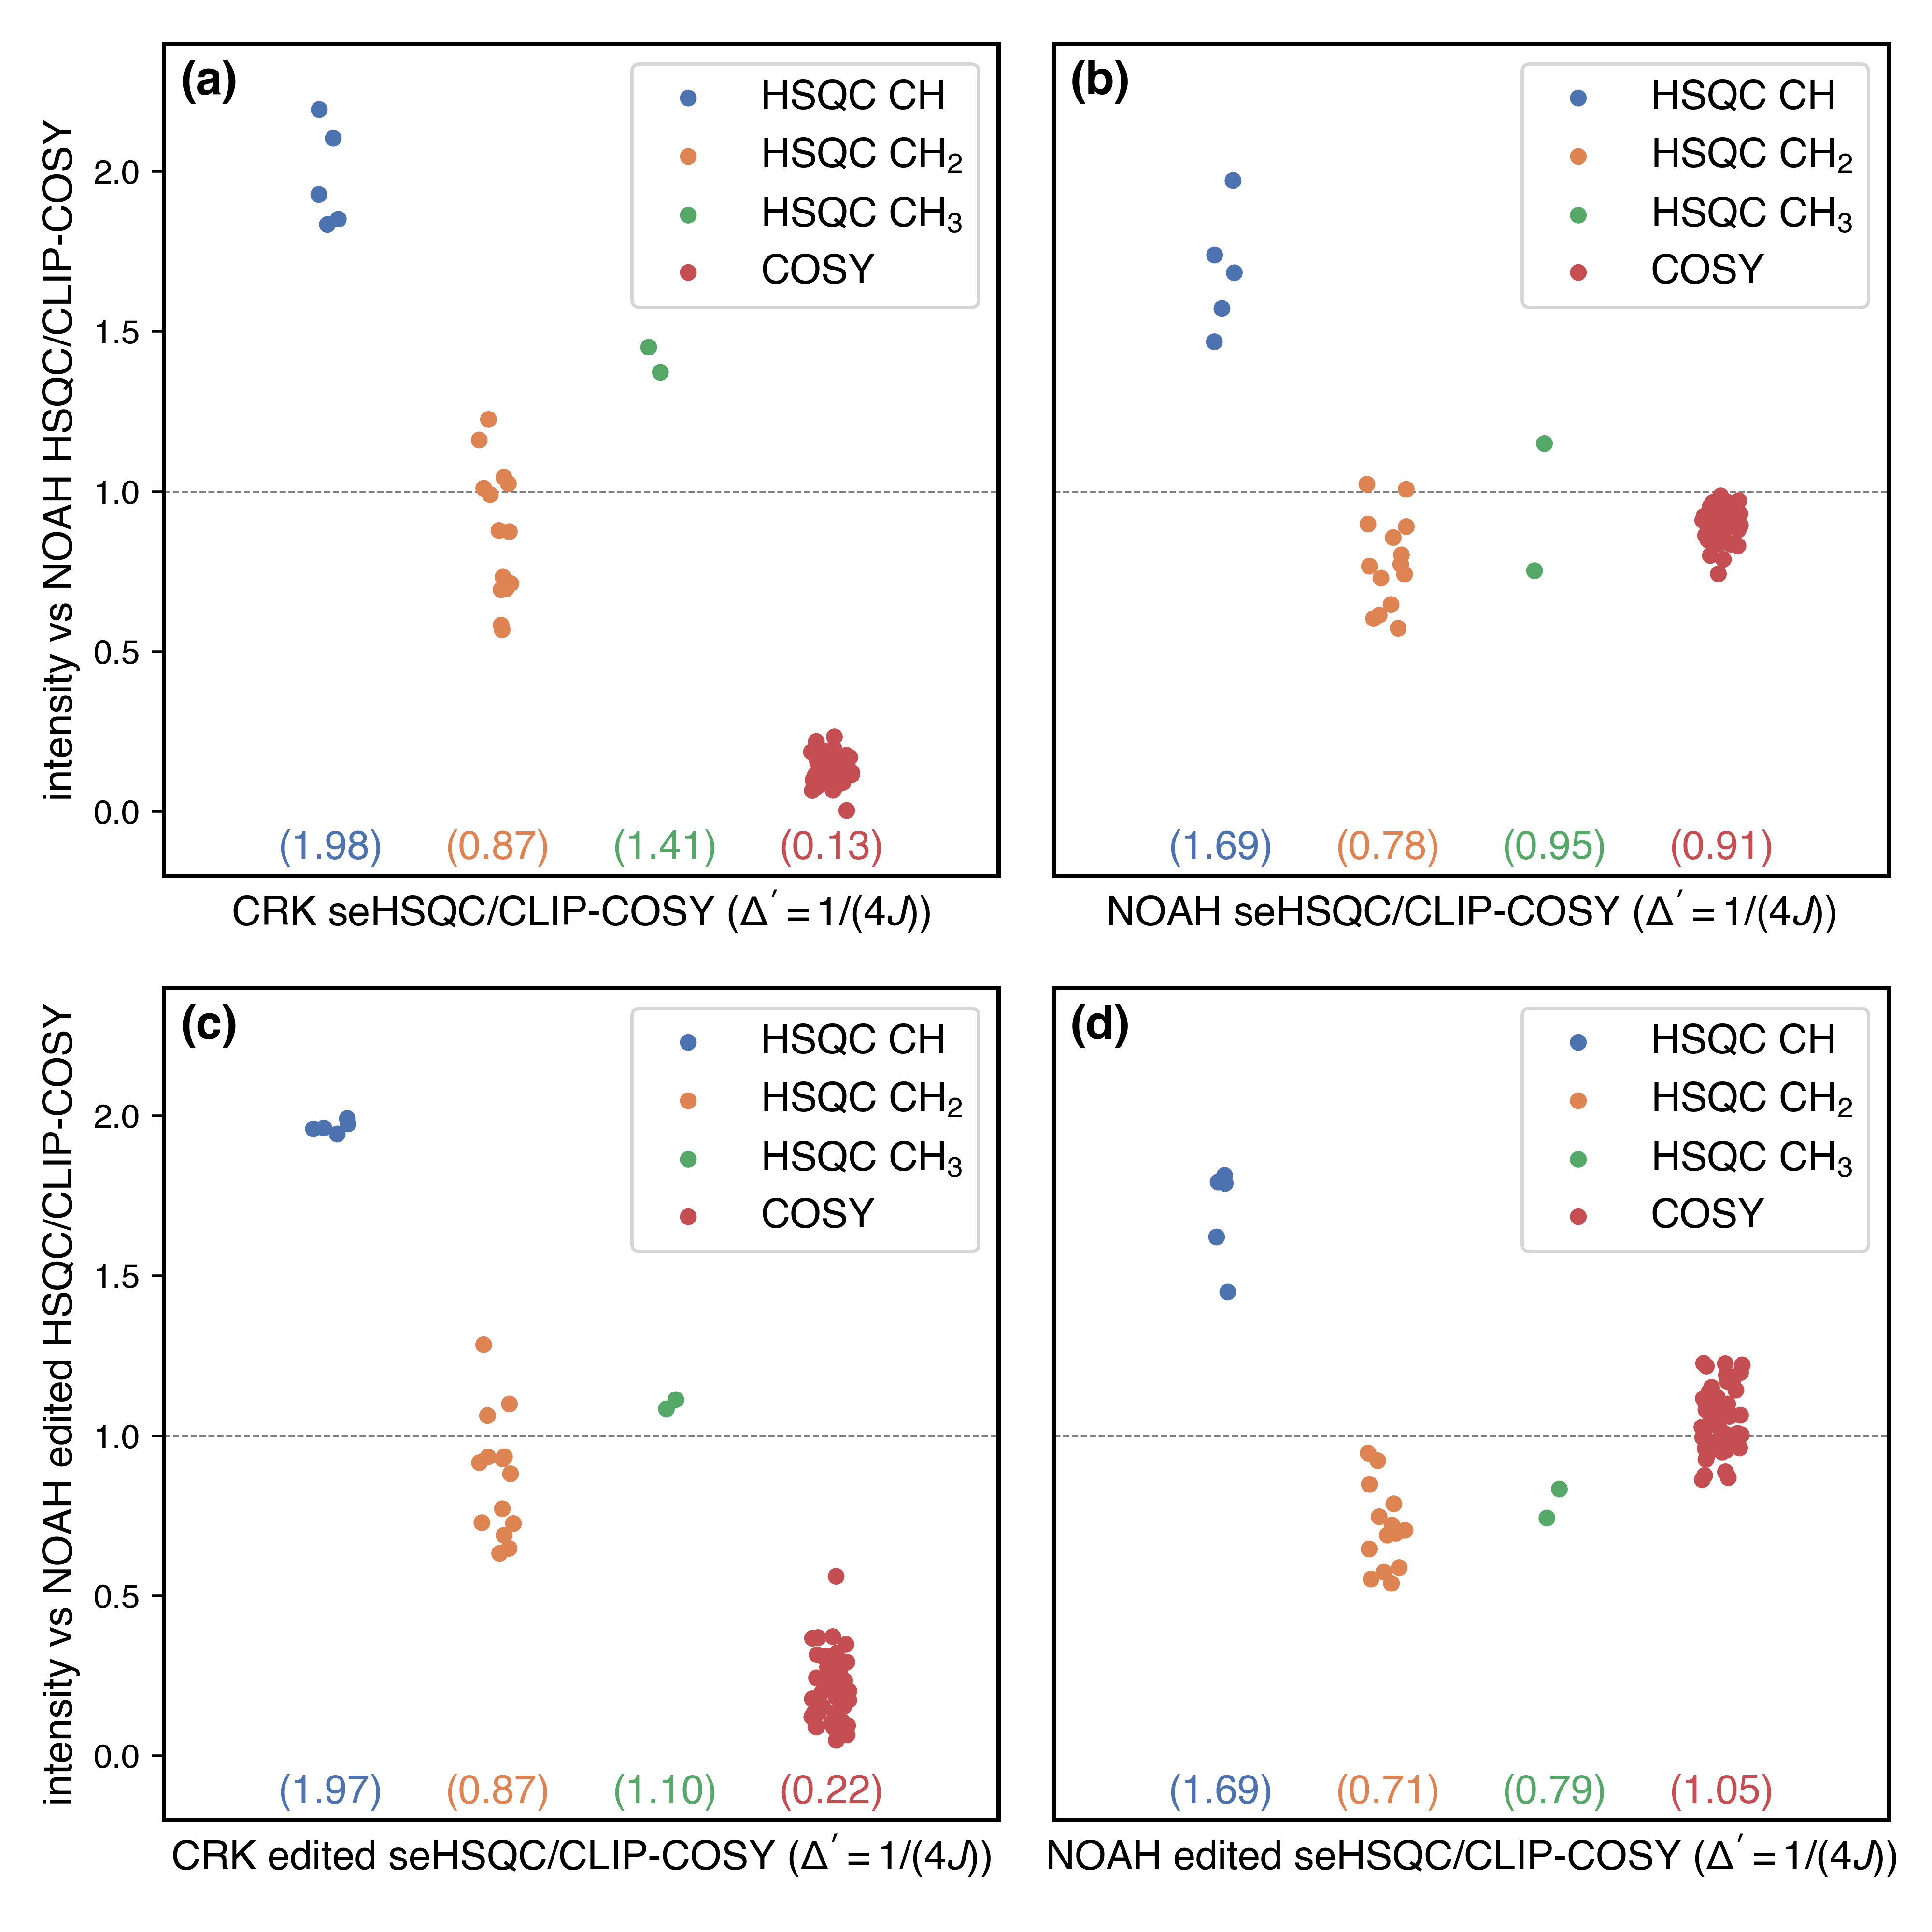
\includegraphics[width=0.8\textwidth]{./figures/combined_1_4j.png}
    \caption{
        Sensitivity of seHSQC sequences with $\Delta'$ set to $1/(4\cdot\onejch)$, versus the corresponding NOAH HSQC/CLIP-COSY supersequence (i.e.\ unedited for (a) and (b), edited for (c) and (d)).
        \textbf{(a)} CRK seHSQC + CLIP-COSY, without multiplicity editing.
        \textbf{(b)} NOAH seHSQC + CLIP-COSY, without multiplicity editing.
        \textbf{(c)} CRK seHSQC + CLIP-COSY, with multiplicity editing.
        \textbf{(d)} NOAH seHSQC + CLIP-COSY, with multiplicity editing.
        \andro{}
    }
    \label{fig:combined_1_4j}
\end{figure}

By setting $\Delta' = 1/(4\cdot\onejch)$, theory predicts a larger sensitivity enhancement for \ce{CH} peaks, whereas \ce{CH2} and \ce{CH3} peaks should have the same sensitivity as in the unenhanced HSQC.
However, for the NOAH seHSQC, we note that the improvements in HSQC \ce{CH} sensitivity gained by moving from $\Delta' = 1/(8\cdot\onejch)$ (\figref{sehsqc_comp}b) to $\Delta' = 1/(4\cdot\onejch)$ (\figref{combined_1_4j}b) are marginal (ca.\ 10\%).
At the same time, for \ce{CH2} and \ce{CH3} peaks, we observe sensitivity \textit{losses} relative to the HSQC; this is likely due to pulse imperfections in the longer pulse sequence and is in line with previous studies (ref.\ \citenum{Schleucher1994JBNMR} of the main text).

\section{Comparison of BIG-BIRD and ISR elements}

The BIG-BIRD element used here was ${45^\circ}_{45^\circ}(\proton{}) - 2\Delta - 180^\circ(\proton{},\carbon{}) - 2\Delta - {45^\circ}_{225^\circ}(\proton{})$ for the unedited NOAH seHSQC, where $\beta_\phi$ indicates a hard pulse with flip angle $\beta$ and phase $\phi$, and $\Delta = 1/(4\cdot\onejch)$.
For the edited NOAH seHSQC, the BIG-BIRD pulse phases are slightly modified to give ${45^\circ}_{315^\circ}(\proton{}) - 2\Delta - 180^\circ(\proton{},\carbon{}) - 2\Delta - {45^\circ}_{135^\circ}(\proton{})$.
These, and the ISR, have the same net effect on \magn{\ce{C}} and \magnnot{\ce{C}} magnetisation, as can be seen from the product operator analysis in \figref{pprogs_prodop}.
However, the ISR provides greater sensitivity in both the HSQC and downstream COSY.

\begin{figure}
    \centering
    % figures/bigbird.py
    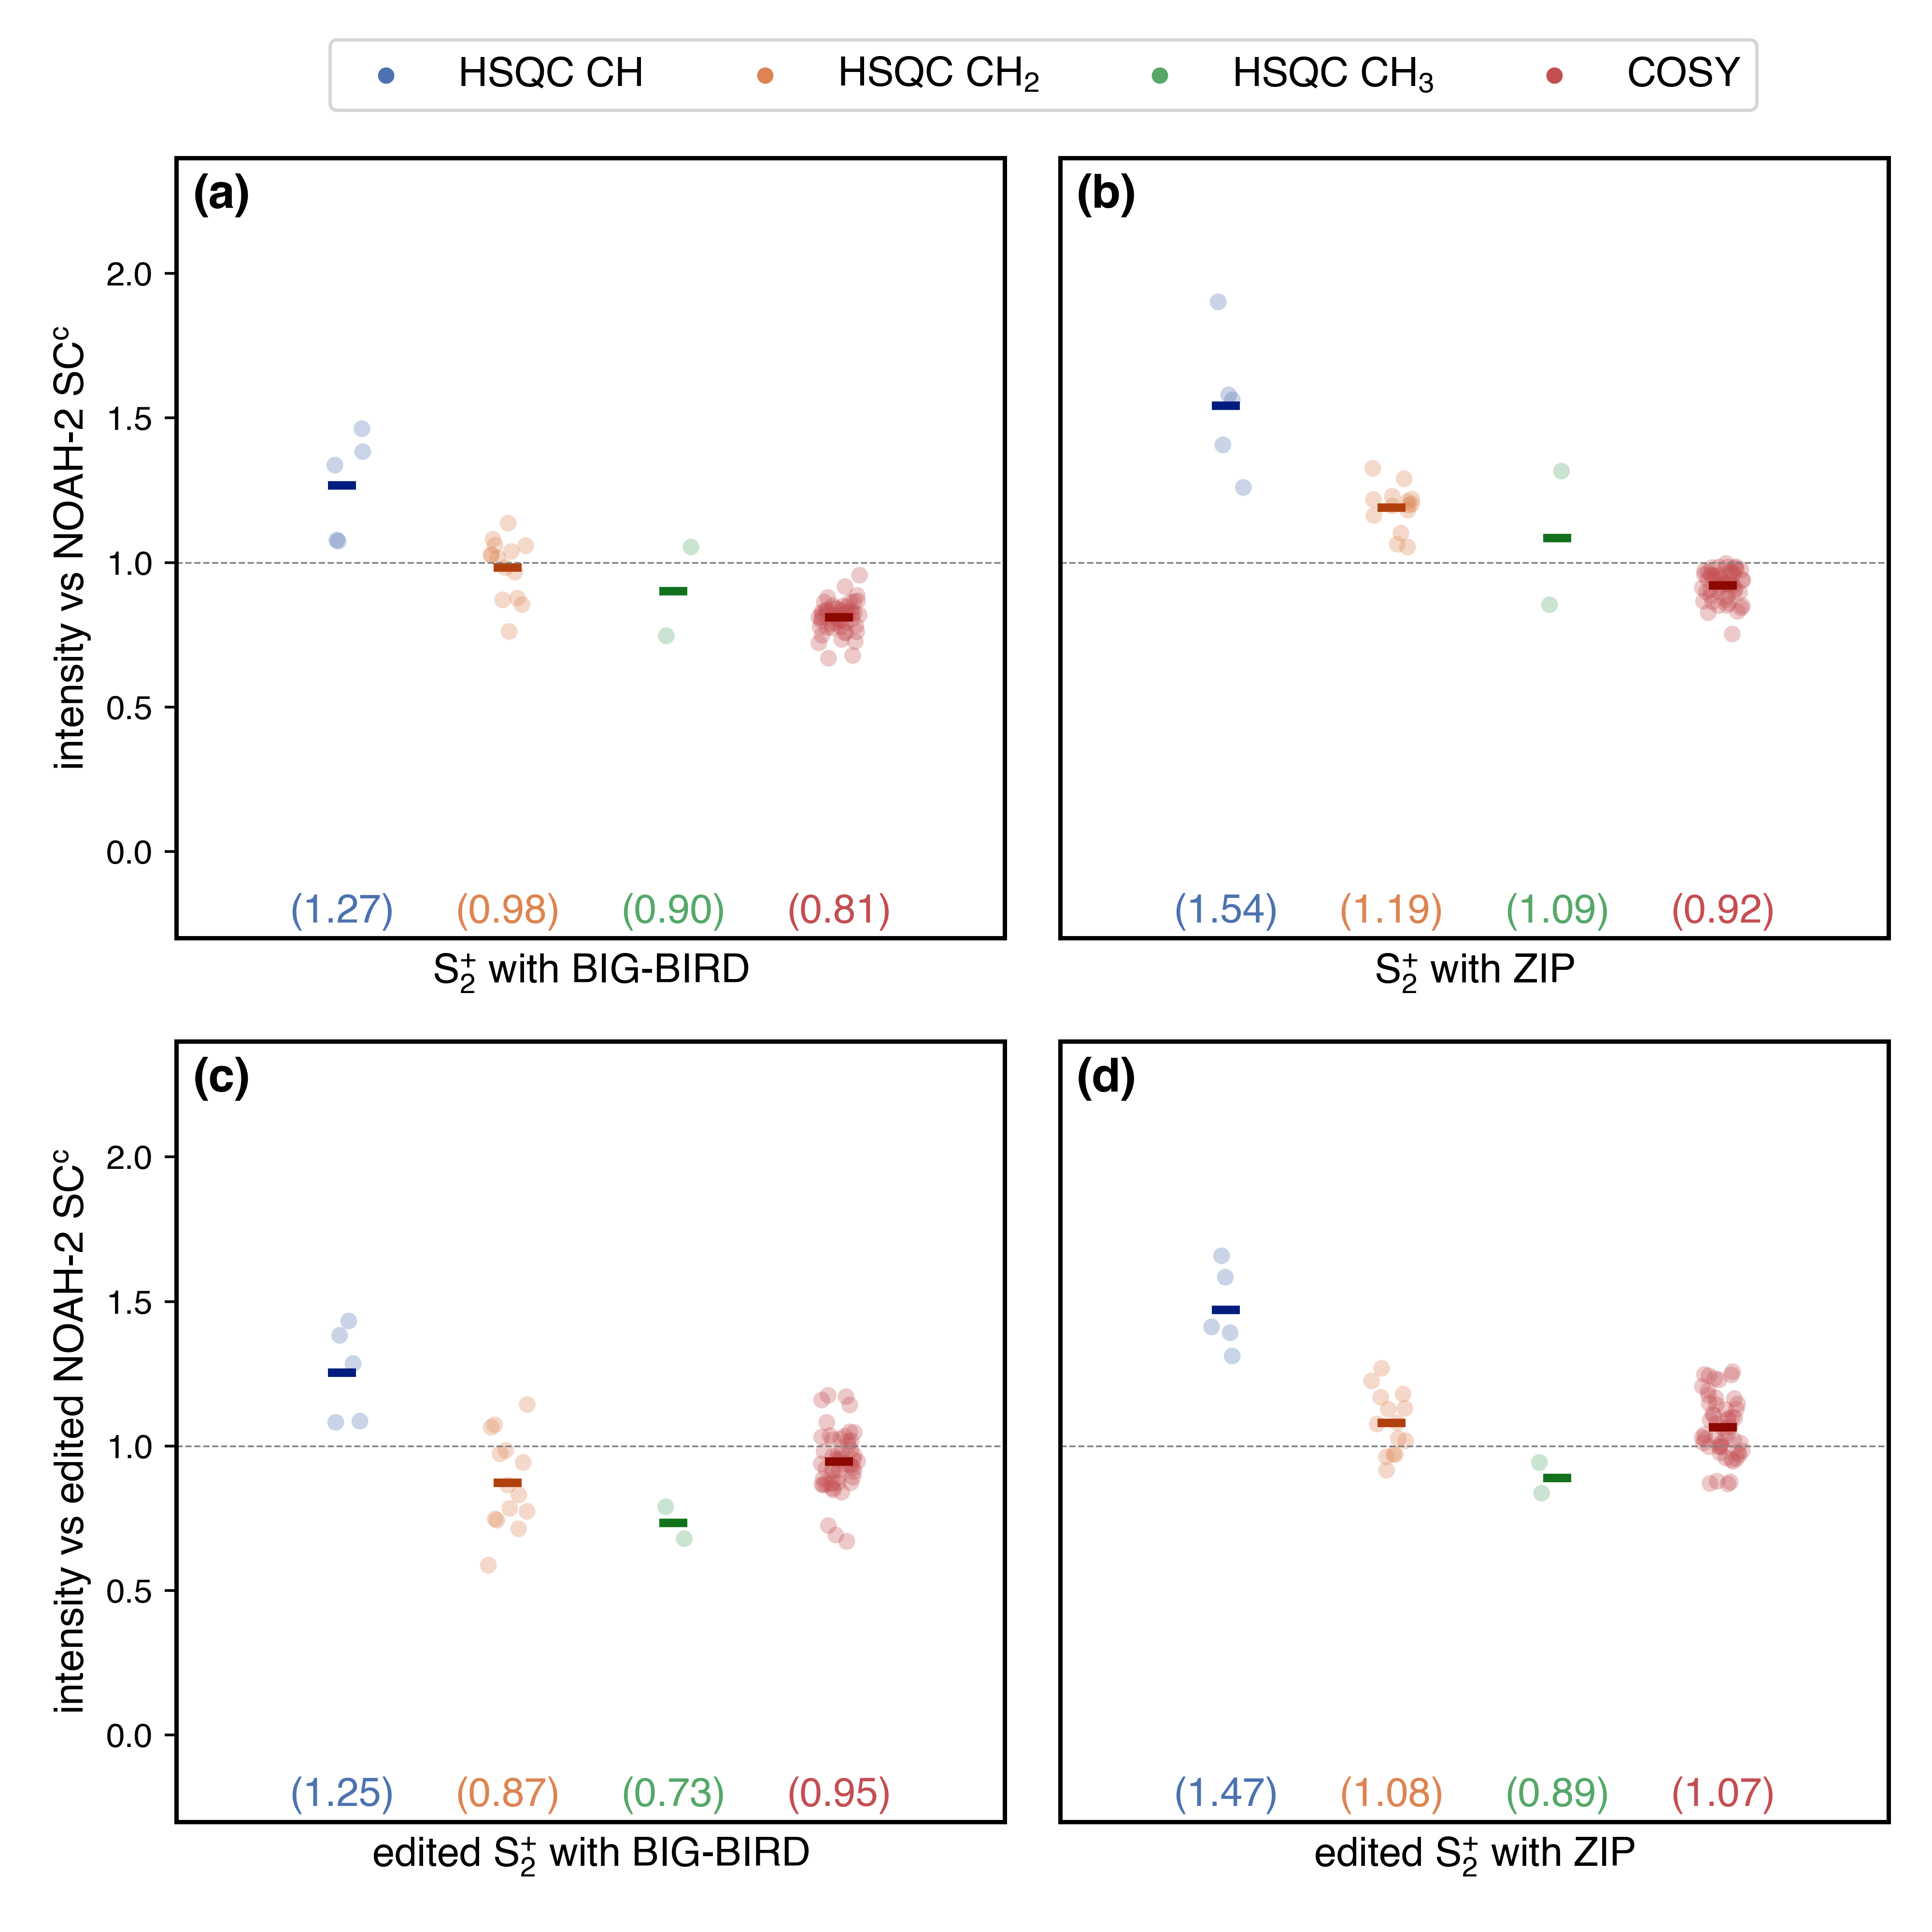
\includegraphics[width=0.8\textwidth]{./figures/bigbird.png}
    \caption{
        Sensitivity of NOAH-2 \noahtwo{Sp}{Cc} supersequences with either BIG-BIRD or ISR elements, versus the corresponding NOAH-2 \noahtwo{S}{Cc} supersequences (i.e.\ unedited for (a) and (b), edited for (c) and (d)).
        \textbf{(a)} Using the unedited NOAH seHSQC with the BIG-BIRD element.
        \textbf{(b)} Unedited seHSQC with ISR.
        \textbf{(c)} Edited seHSQC with BIG-BIRD.
        \textbf{(d)} Edited seHSQC with ISR.
        \andro{}
    }
    \label{fig:bigbird}
\end{figure}


\section{Origin and suppression of wing artefacts}

The origin of the ``wing'' artefacts in the final homonuclear modules can be most clearly seen from the following series of experiments involving the NOAH-3 \nitrogen{} seHSQC/\carbon{} seHSQC/CLIP-COSY (\noahthree{Spn}{Sp}{Cc}) supersequence.
Since the $f_1$ spectral windows of the two seHSQC modules are different, they lead to distinct sets of wing artefacts in the COSY if the extra gradient before $t_1$ is not present.
As described in the main text, each peak in the COSY with an indirect-dimension frequency of $f_1 = \Omega_{\ce{H}}$ is flanked by a pair of artefacts at
\begin{align*}
    f_1 &= \Omega_{\ce{H}} \pm \Omega_{\ce{H}} \cdot \left(\frac{\mathrm{SW_{COSY}}}{2 \cdot \mathrm{SW_{HSQC}}}\right),
\end{align*}

where $\Omega_{\ce{H}}$ is the offset of the relevant proton and $\mathrm{SW}$ refers to the indirect-dimension spectral width.
In the spectra shown in the following figures, we have
\begin{align*}
    \mathrm{SW_{\ce{^15N}\,HSQC}} &= \SI{2128}{\Hz} \\
    \mathrm{SW_{\ce{^13C}\,HSQC}} &= \SI{23810}{\Hz} \\
    \mathrm{SW_{COSY}}            &= \SI{8418}{\Hz}
\end{align*}

meaning that the artefacts coming from the \nitrogen{} seHSQC occur at $f_1 = (1.00 \pm 1.98) \Omega_{\ce{H}}$ (and are therefore often folded), whereas artefacts coming from the \carbon{} seHSQC occur at $f_1 = (1.00 \pm 0.18) \Omega_{\ce{H}}$ (and are typically found very close to the main peak).
In both cases, the artefacts associated with intense methyl group peaks are the most obvious, but similar artefacts are observed for all other peaks, albeit with lower absolute intensities.

\begin{figure}
    \centering
    % figures/wing_artefacts.py
    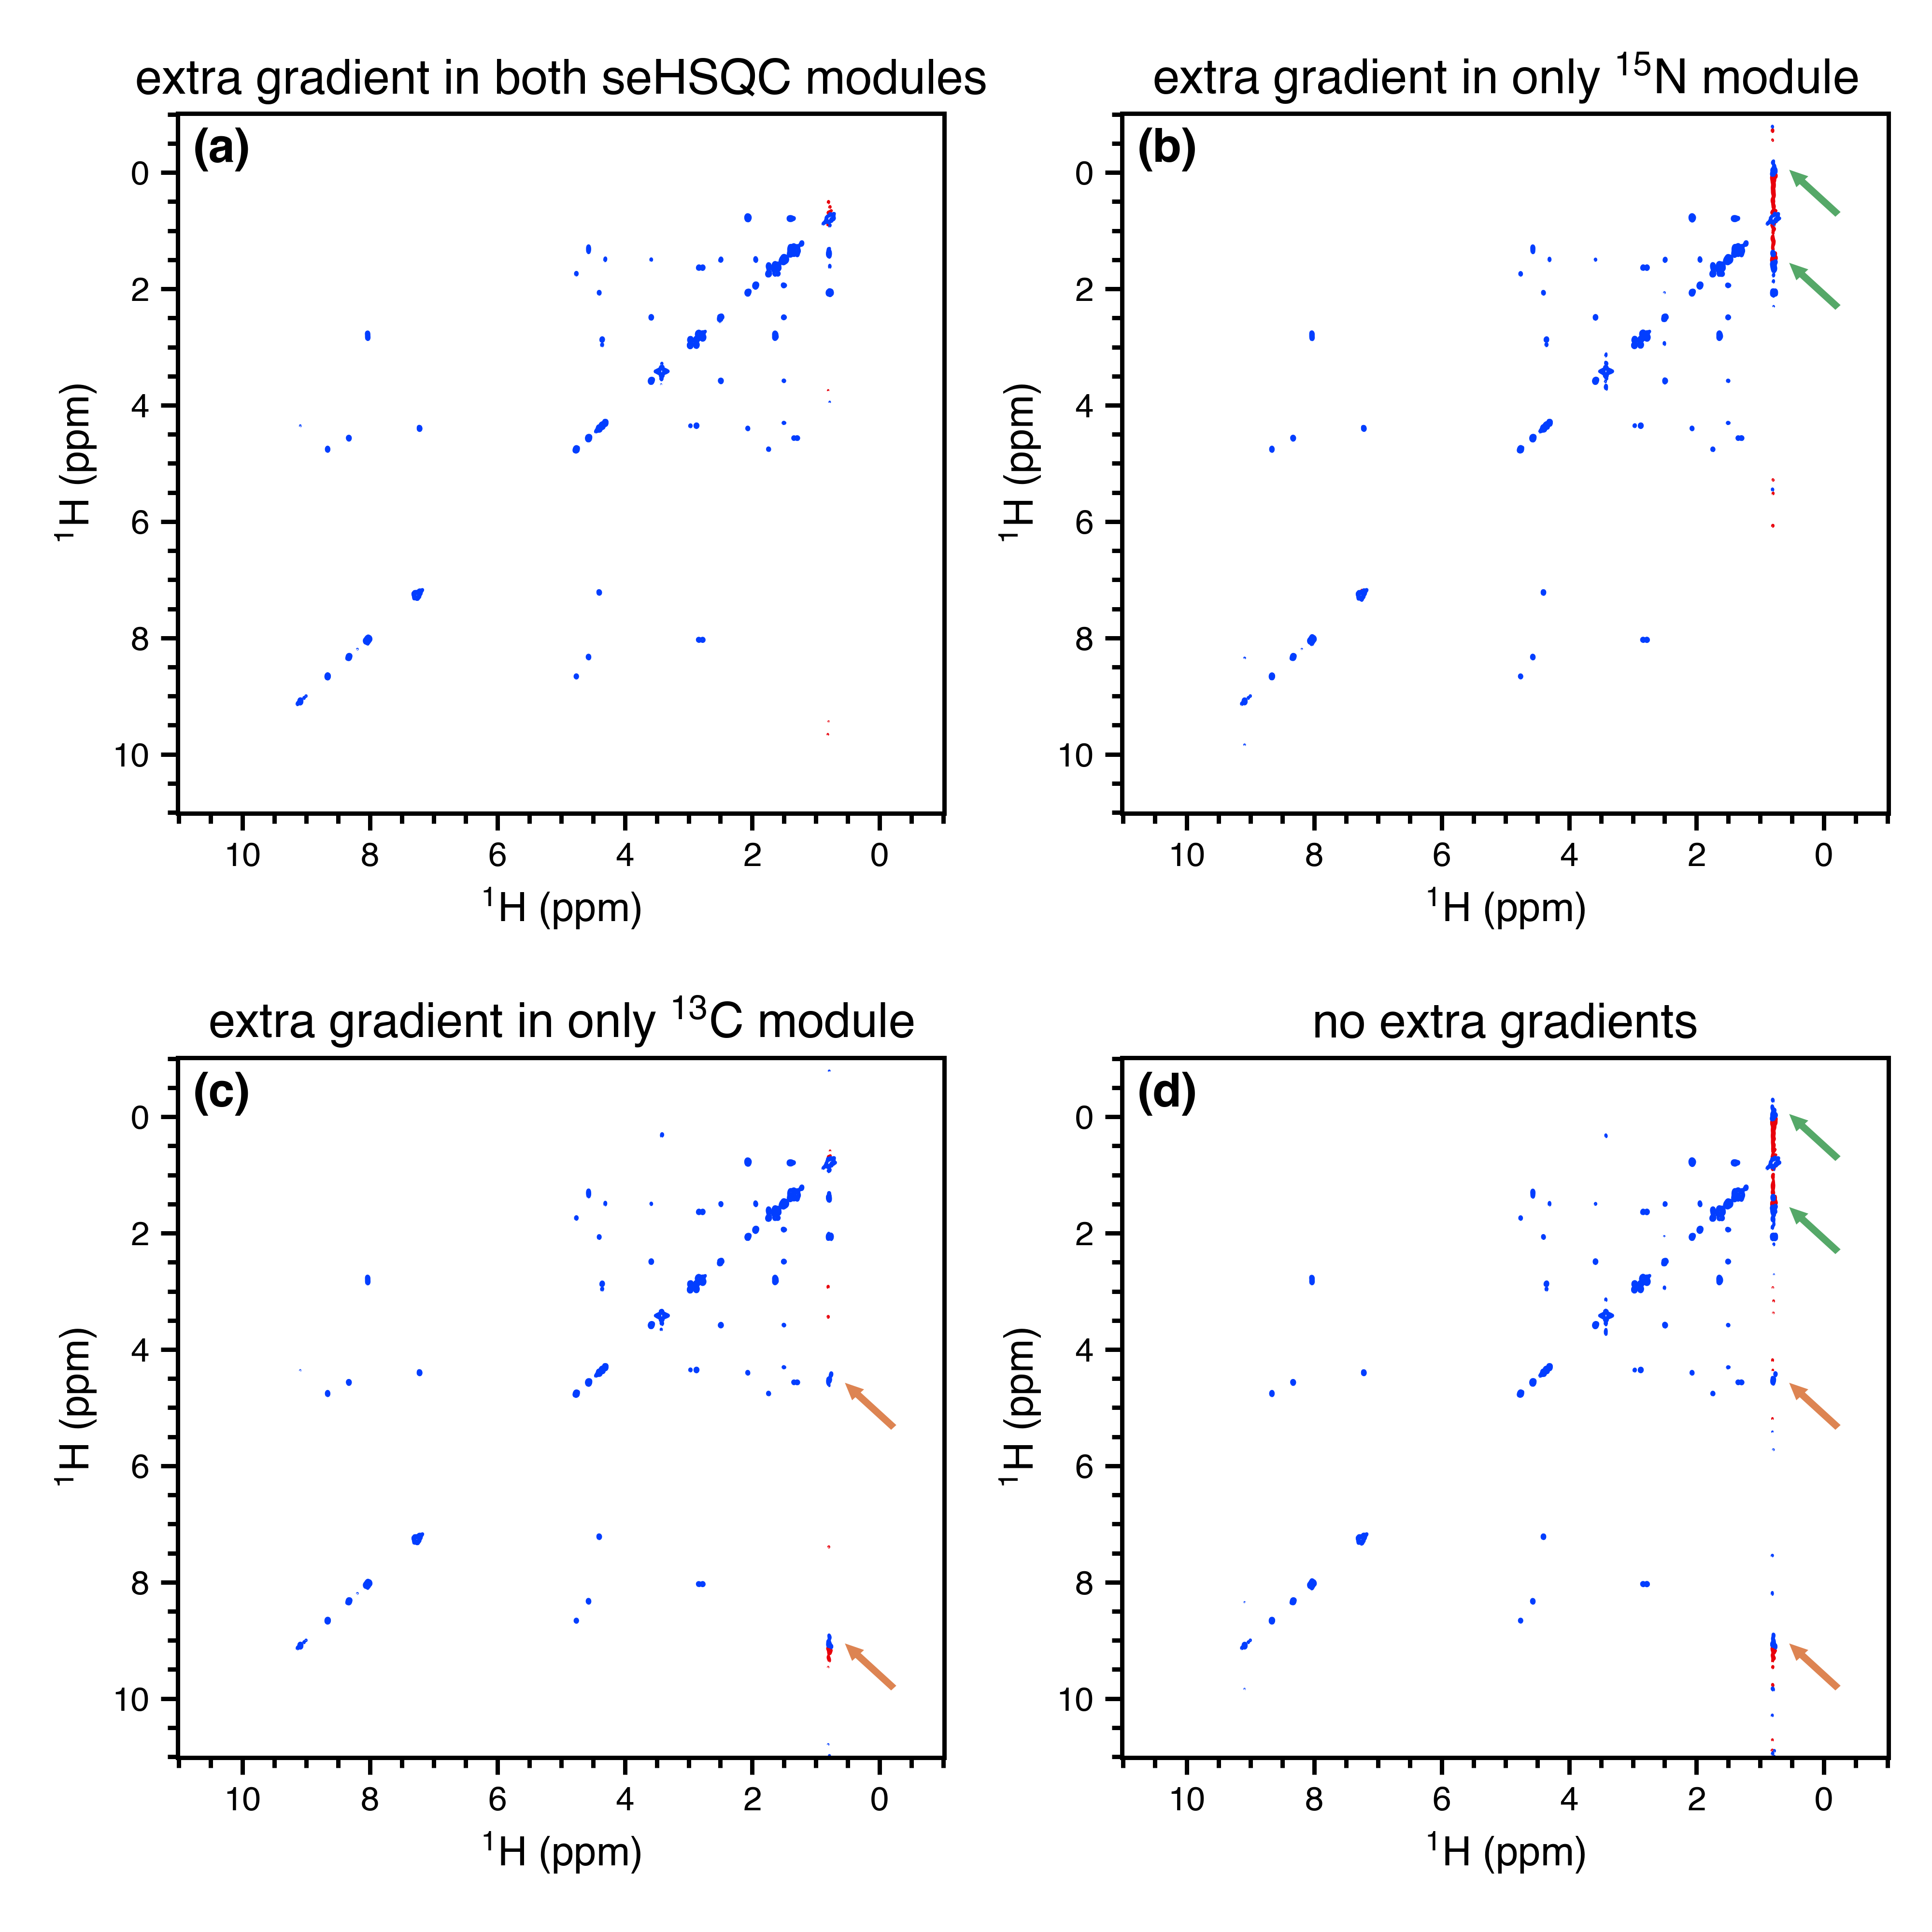
\includegraphics[width=0.8\textwidth]{./figures/wing_artefacts.png}
    \caption{
        CLIP-COSY spectra obtained from various forms of the NOAH-3 \noahthree{Spn}{Sp}{Cc} supersequence.
        Wing artefacts arising from the \nitrogen{} seHSQC are highlighted in orange; those arising from the \carbon{} seHSQC in green.
        Notice how (in this case) the former can easily be misinterpreted as a crosspeak, while the latter obscures genuine crosspeaks.
        \textbf{(a)} With the extra gradient inserted for both modules, i.e.\ no artefacts.
        \textbf{(b)} With an extra gradient in only the \nitrogen{} module, i.e.\ only the \carbon{} artefacts.
        \textbf{(c)} With an extra gradient in only the \carbon{} module.
        \textbf{(d)} With no extra gradients.
        \grami{}
    }
    \label{fig:wing_artefacts}
\end{figure}

\begin{figure}
    \centering
    % figures/wing_artefacts2.py
    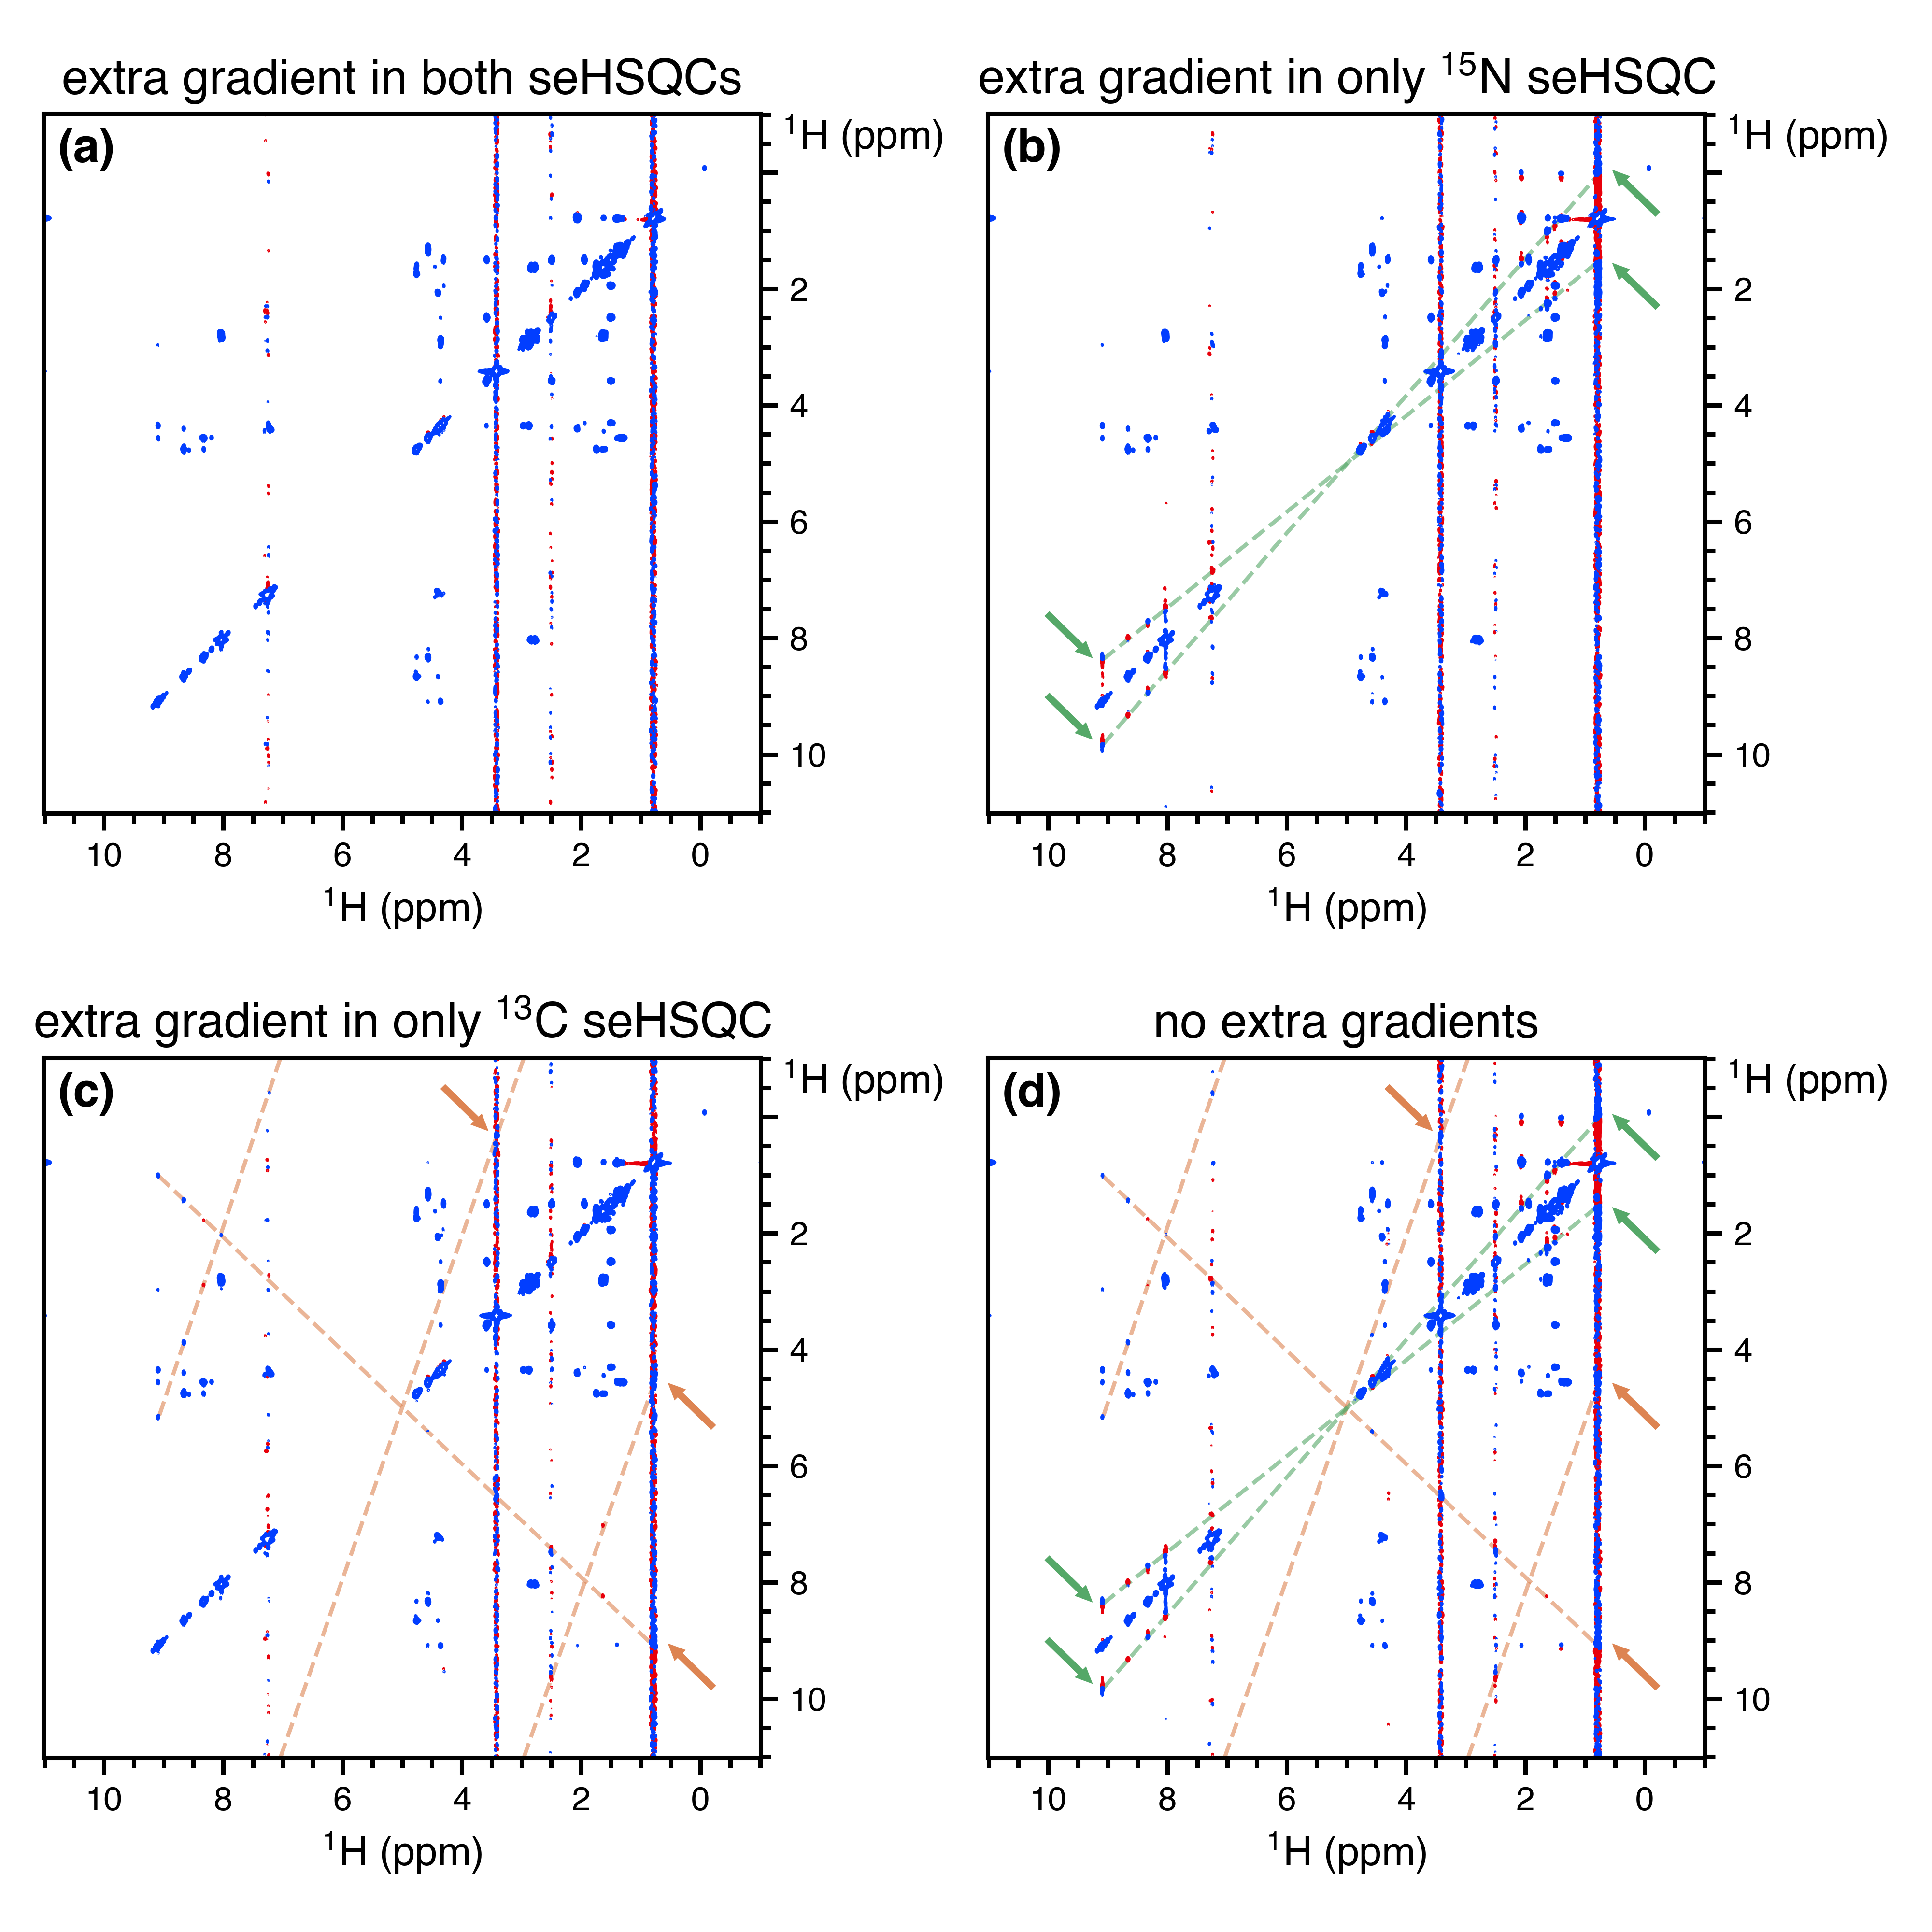
\includegraphics[width=0.8\textwidth]{./figures/wing_artefacts2.png}
    \caption{
        The same spectra as \figref{wing_artefacts}, but plotted with a smaller base contour level to illustrate the regular indirect-dimension frequencies of the wing artefacts.
        A greater number of artefacts are now visible (in addition to those already highlighted in \figref{wing_artefacts}, which are still marked with arrows).
        The artefacts arising from the \nitrogen{} seHSQC lie on the orange dotted line; those arising from the \carbon{} seHSQC lie on the green dotted line.
        \textbf{(a)} With the extra gradient inserted for both modules, i.e.\ no artefacts.
        \textbf{(b)} With an extra gradient in only the \nitrogen{} module, i.e.\ only the \carbon{} artefacts.
        \textbf{(c)} With an extra gradient in only the \carbon{} module.
        \textbf{(d)} With no extra gradients.
        \grami{}
    }
    \label{fig:wing_artefacts2}
\end{figure}

\clearpage

Additional information can be gleaned from the following series of CLIP-COSY spectra, obtained from NOAH-2 \noahtwo{Sp}{Cc} supersequences.
In the seHSQC module, the two gradients $g_1$ in the $t_1$ period are independently enabled or disabled (by setting their amplitude to 0).
Traces of the resulting CLIP-COSY spectra are shown in \figref{wing_gradients}.
The gradients serve to dephase any bulk \magnnot{\ce{C}} magnetisation that is transverse during either half of $t_1$: therefore, if (for example) the gradient in the first half of $t_1$ is switched off, this allows bulk magnetisation that is transverse in the first half of $t_1$ to evolve and ultimately contribute to the wing artefacts in the CLIP-COSY.
As can be seen, gradients must be applied in \textit{both} halves for complete suppression of the wing artefacts.

\begin{figure}
    \centering
    
\includegraphics{./figures/andro.png}

    % figures/wing_gradients.py
    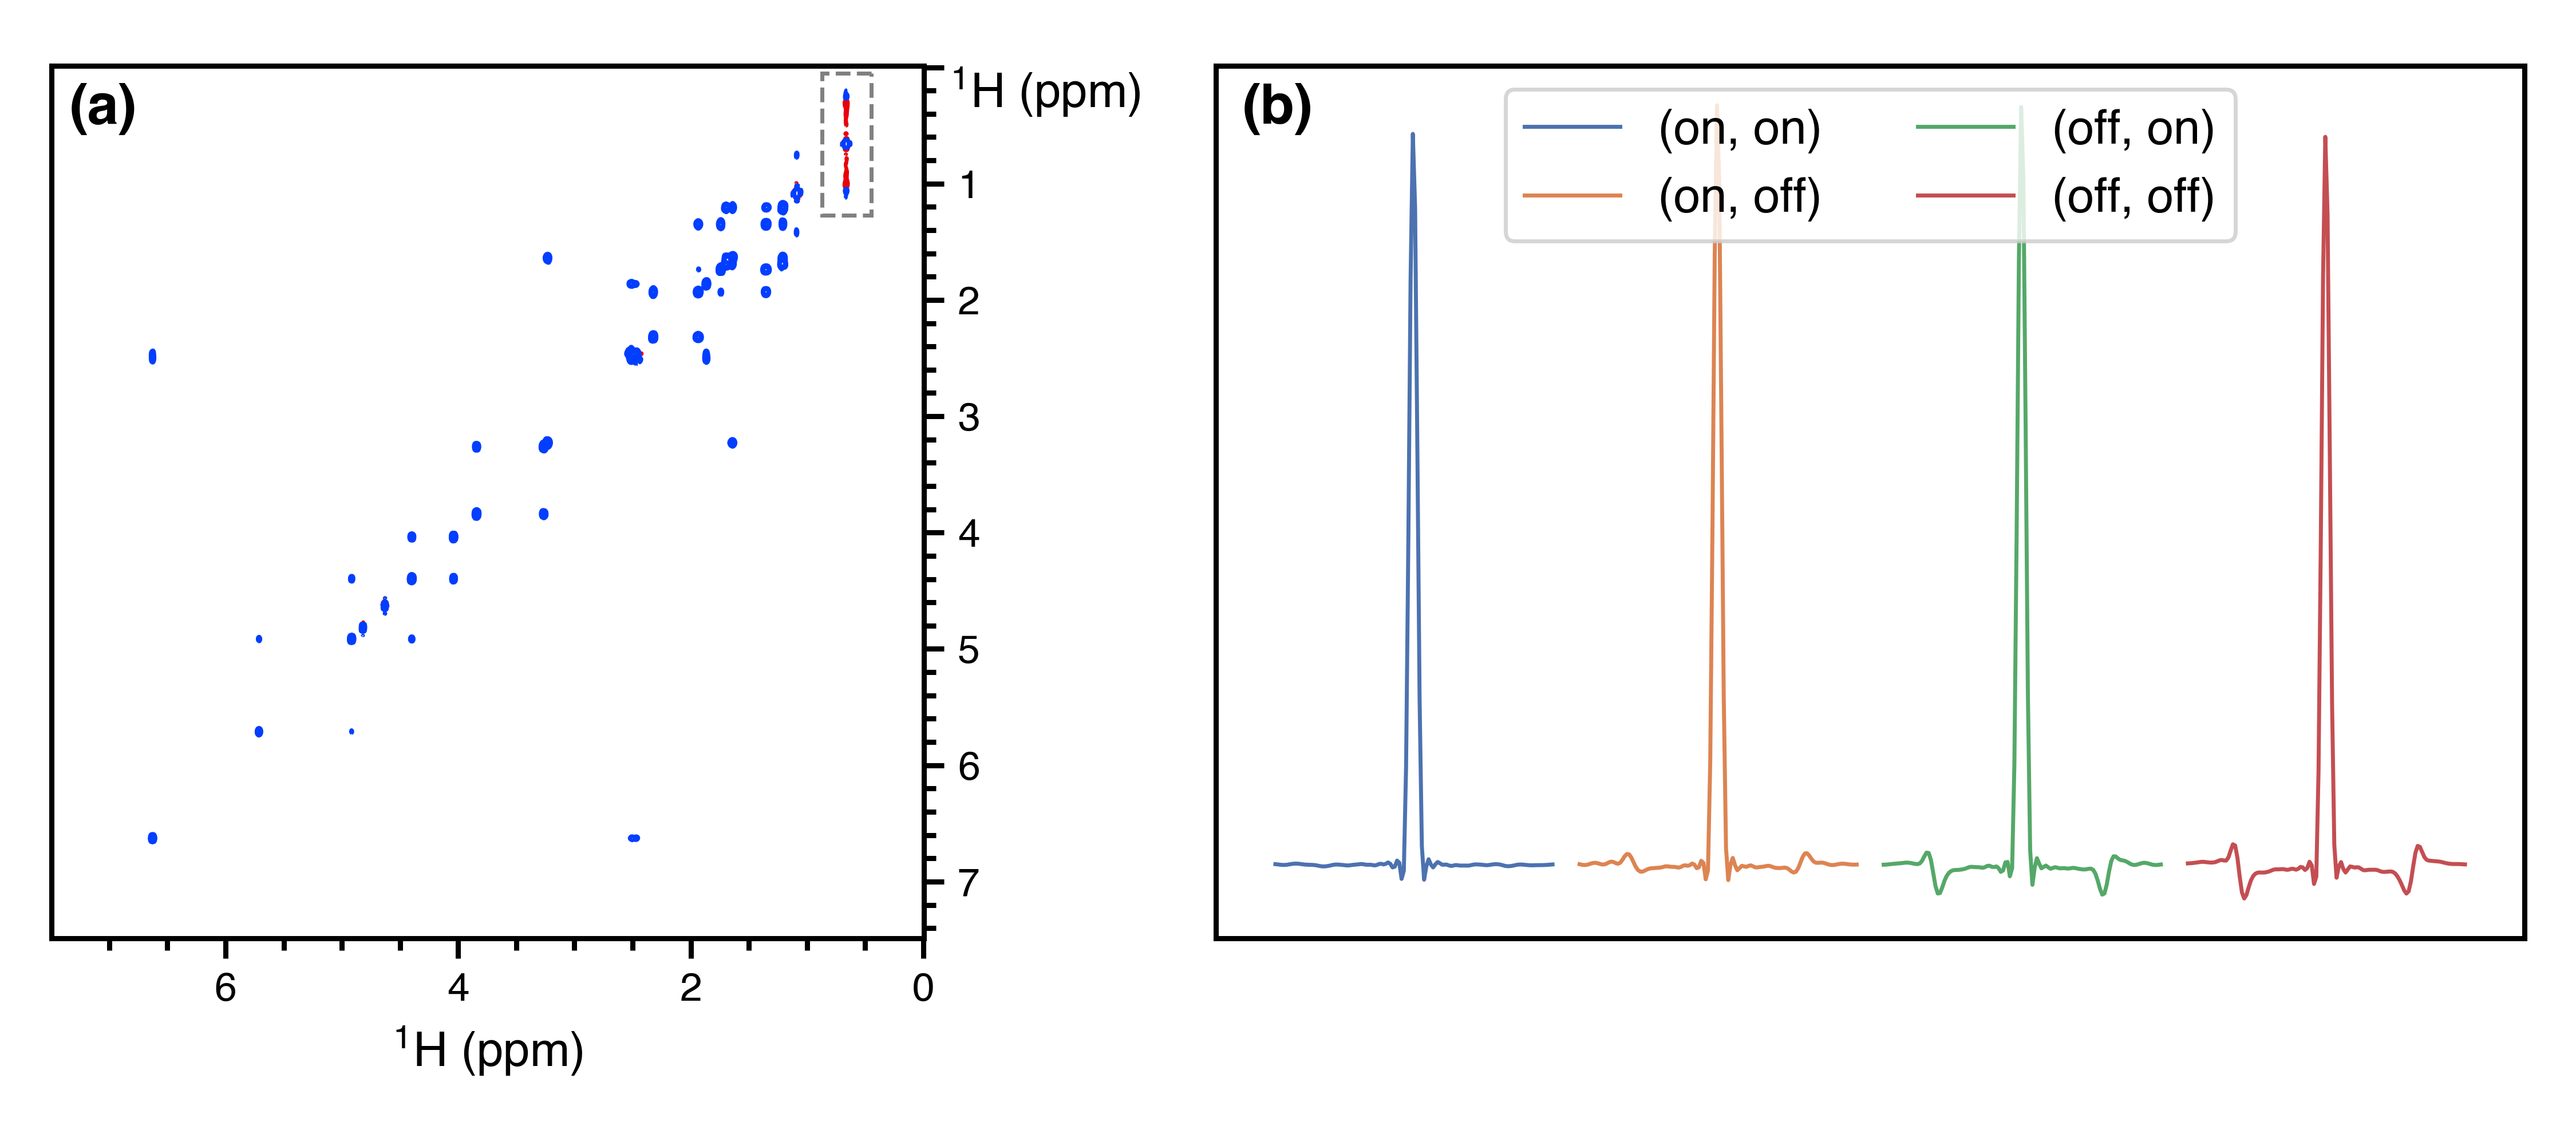
\includegraphics[width=0.8\textwidth]{./figures/wing_gradients.png}
    \caption{
        \textbf{(a)} CLIP-COSY spectrum obtained from NOAH-2 \noahtwo{Sp}{Cc} sequence, where both gradients in $t_1$ were disabled (i.e.\ ``(off, off)'').
        The other three CLIP-COSY spectra are similar, except that the (on, on) spectrum (with gradients applied in both halves of $t_1$) does not have wing artefacts (grey box).
        \textbf{(b)} $f_1$ traces through \SI{0.67}{\ppm} of the four CLIP-COSY spectra obtained with various combinations of gradients, corresponding to the boxed area in (a).
        Only the (on, on) spectrum (in blue) is free from wing artefacts.
        The (on, off) and (off, on) spectra (in orange and green respectively) have wing artefacts arising from bulk magnetisation that evolves during the second and first halves of the seHSQC $t_1$ period respectively.
        The (off, off) spectrum (red), which corresponds to the 2D spectrum in (a), has the greatest intensity of wing artefacts.
        \andro{}
    }
    \label{fig:wing_gradients}
\end{figure}


\section{Retention of bulk magnetisation by \texorpdfstring{\nitrogen{}}{15N} modules}

\begin{figure}
    \centering
    % figures/n15_bulk_retention.py
    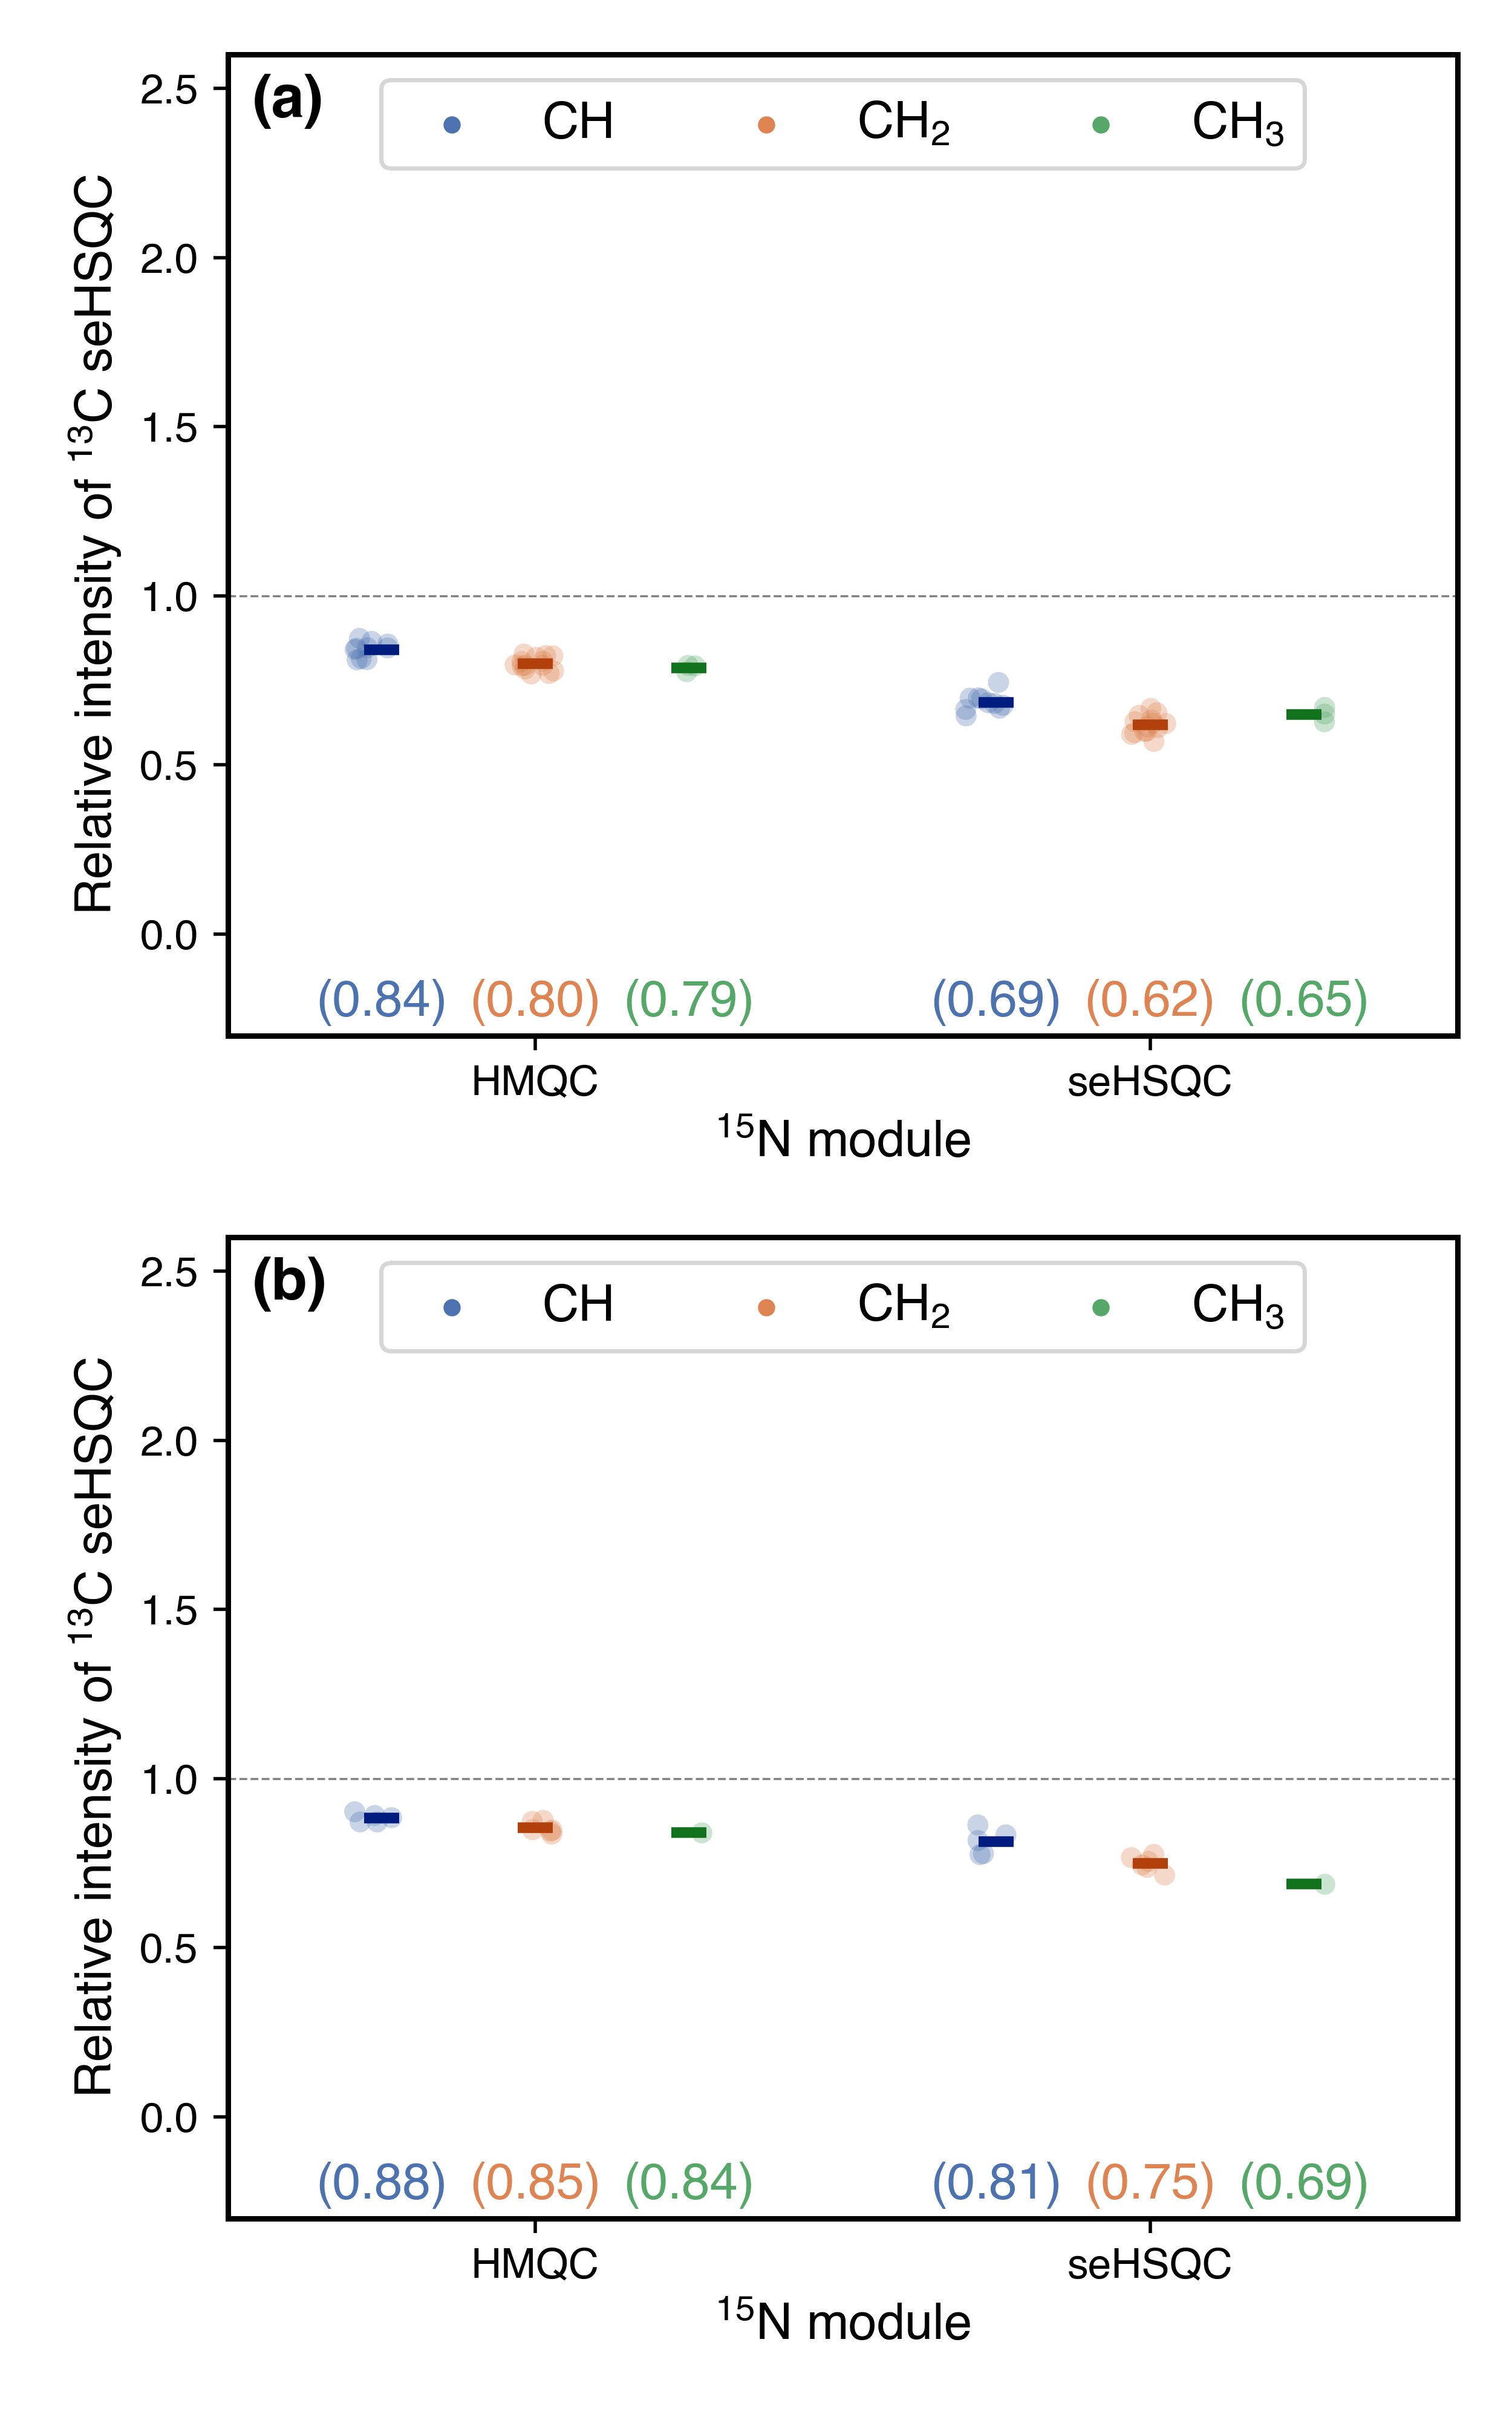
\includegraphics[width=0.5\textwidth]{./figures/n15_bulk_retention.png}
    \caption{
        Signal intensities of the \carbon{} seHSQC in NOAH-3 \noahthree{X}{Sp}{Cc} supersequences, normalised against a reference \carbon{} seHSQC taken from a NOAH-2 \noahtwo{Sp}{Cc} supersequence.
        The module \noahX{} is either the \nitrogen{} HMQC (\noahM{}) or the \nitrogen{} seHSQC (\noahSpn{}); the numbers indicate the amount of \magn{\ce{C}} magnetisation that is preserved by the \nitrogen{} module.
        \textbf{(a)} Using \SI{40}{\milli\molar} gramicidin in DMSO-$d_6$.
        \textbf{(b)} Using \SI{50}{\milli\molar} zolmitriptan in DMSO-$d_6$.
        Spectra were obtained on a \SI{700}{\MHz} Bruker AV III equipped with a TCI H/C/N cryoprobe.
    }
    \label{fig:n15_bulk_retention}
\end{figure}


\section{\texorpdfstring{\nitrogen{}}{15N} HSQC and line broadening}

For \nitrogen{}--\proton{} correlations, both the HMQC and the new seHSQC module are recommended as they keep the bulk magnetisation (both \magn{\ce{C}} and \magnnot{\ce{X}}) along $\pm z$ during the $t_1$ period.
The HSQC module places this magnetisation in the $xy$-plane during $t_1$, leading to $\jhh$ evolution; consequently, the amount of bulk magnetisation ``passed on'' to the downstream modules decreases as the \nitrogen{} $t_1$ is increased.
Since $t_1$ for each NOAH module is incremented in sync, this is manifested in downstream modules as a $t_1$-dependent decrease in amplitude, or $f_1$ line broadening after Fourier transformation, as shown in \figref{n15_linebroadening}.

\begin{figure}
    \centering
    % figures/n15_linebroadening.py
    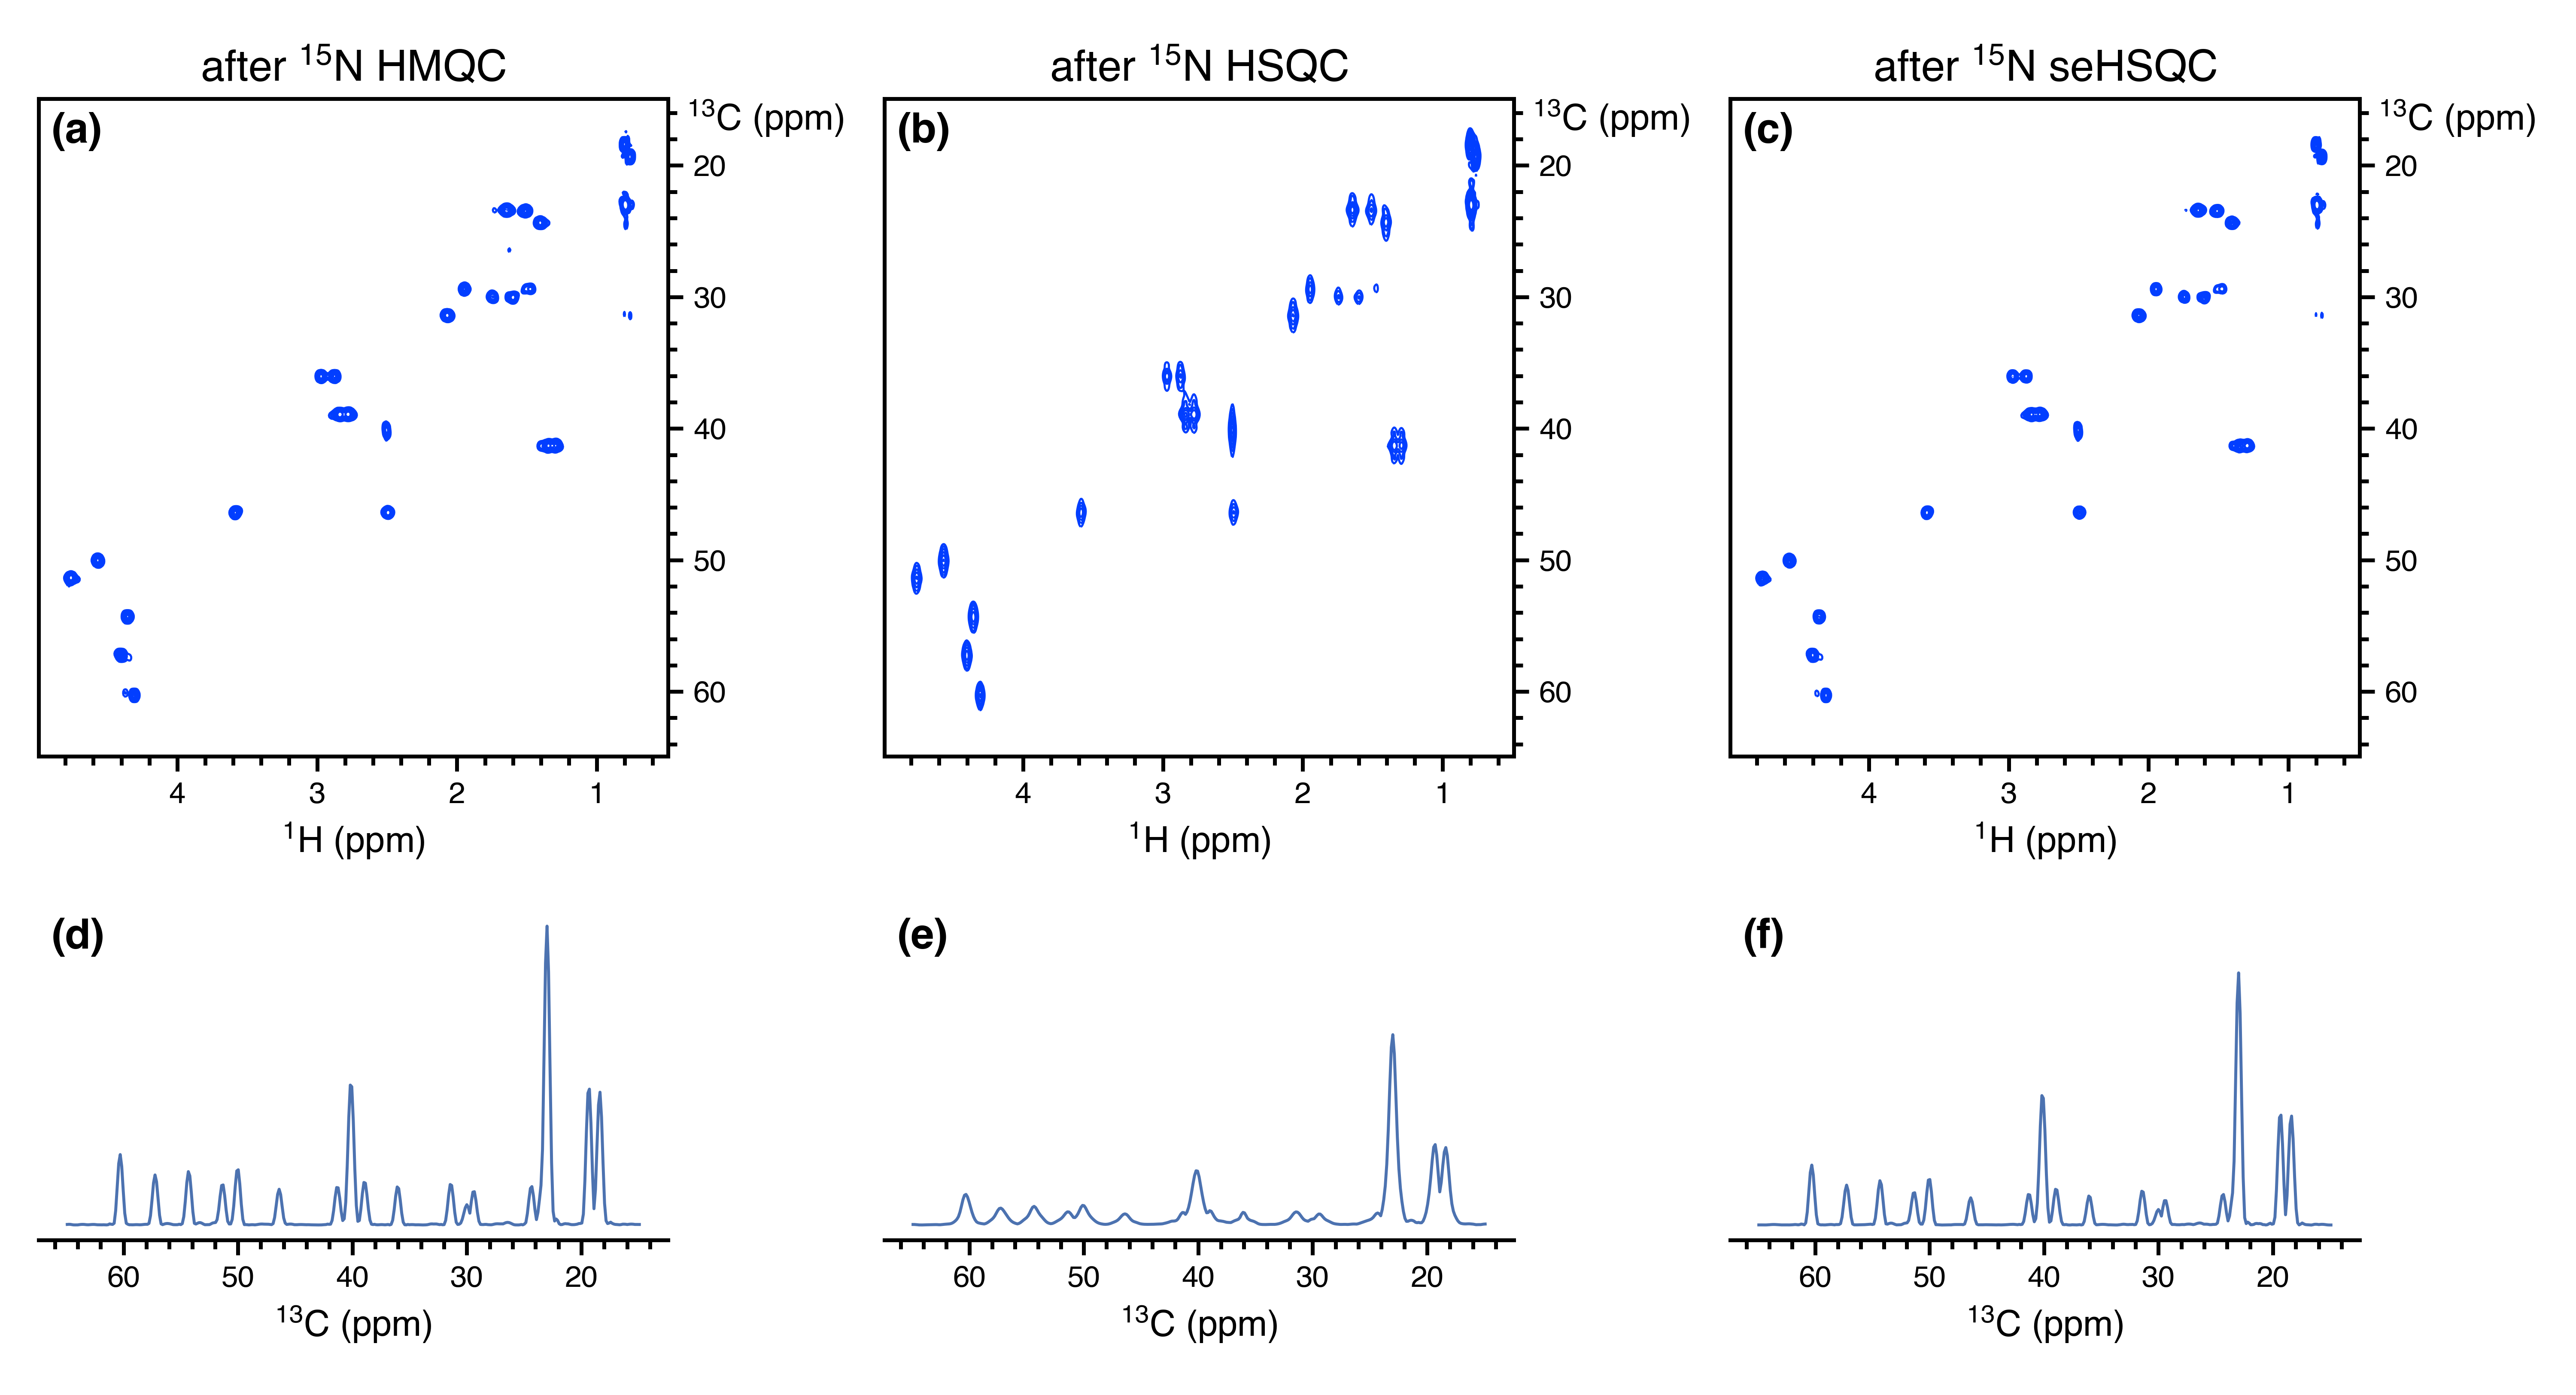
\includegraphics[width=\textwidth]{./figures/n15_linebroadening.png}
    \caption{
        \carbon{} seHSQC spectra obtained from NOAH-3 \noahthree{X}{Sp}{Cc} (\nitrogen{} module + \carbon{} seHSQC + CLIP-COSY) supersequences.
        The \nitrogen{} spectral window was \SI{30}{ppm} and 256 $t_1$ increments were collected, corresponding to an indirect-dimension \nitrogen{} acquisition time of \SI{60.1}{\ms}.
        \textbf{(a)} X = HMQC.
        \textbf{(b)} X = HSQC.
        \textbf{(c)} X = seHSQC.
        \textbf{(d)}--\textbf{(f)} Projections of spectra \textbf{(a)}--\textbf{(c)} onto the $f_1$ axis.
        Note the $f_1$ line broadening in (b) and (e).
        \grami{}
    }
    \label{fig:n15_linebroadening}
\end{figure}

This line broadening also leads to a substantial sensitivity loss (for example, across all peaks, the \carbon{} seHSQC in \figref{n15_linebroadening}b has almost 65\% lower sensitivity than that in \figref{n15_linebroadening}a).
The extent of the line broadening depends on the acquisition time, and is particularly pronounced for long acquisition times, i.e.\ small \nitrogen{} spectral windows.
In our experience, at \nitrogen{} acquisition times of ca.\ \SI{5}{\ms} the effect is almost indiscernible.
Such a short acquisition time would lead to poor resolution in the \nitrogen{} dimension itself, which may or may not be tolerable.
Of course, this issue can be entirely avoided by using either the HMQC or seHSQC.

\section{Effect of lengthened gradients in \texorpdfstring{\nitrogen{}}{15N} modules}

\begin{figure}
    \centering
    
\includegraphics[scale=0.9]{./figures/zolmi.png}\phantom{aaaaaa}

    % figures/cnst16_diff.py
    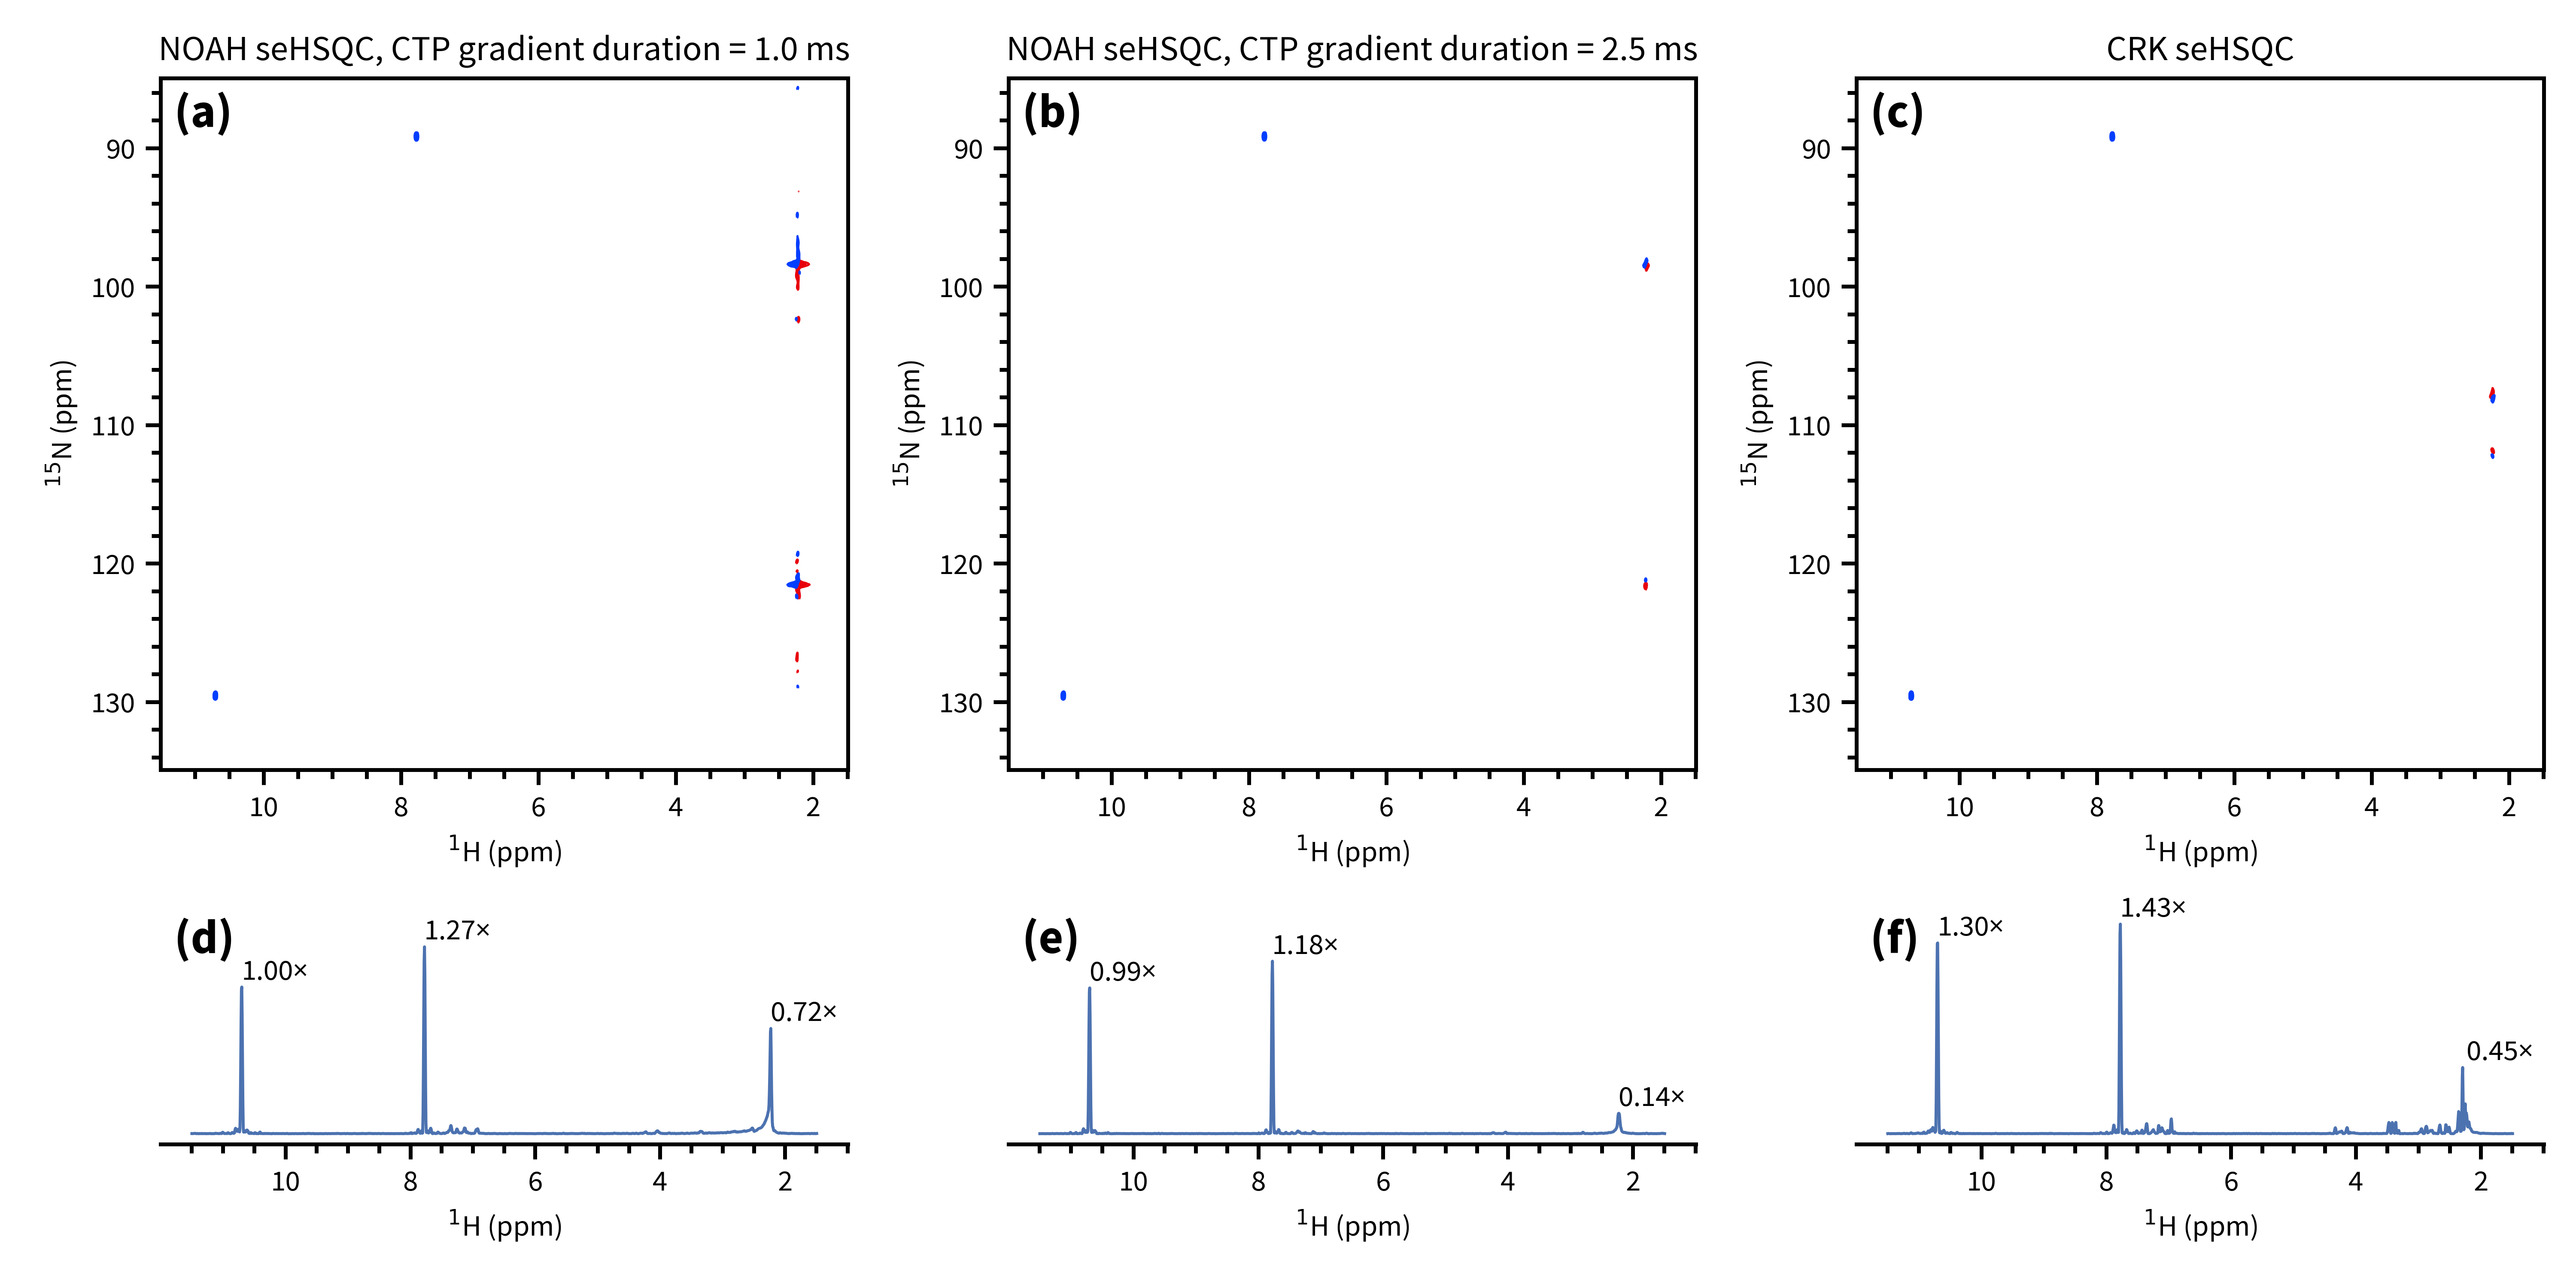
\includegraphics[width=\textwidth]{./figures/cnst16_diff.png}
    \caption{
        \nitrogen{} seHSQC spectra obtained using the NOAH and CRK implementations.
        The peaks at 7.8 and \SI{10.7}{\ppm} (\proton{} shifts) are genuine crosspeaks; the mixed-phase peaks at \SI{2.2}{\ppm} are artefacts.
        The 1D \proton{} spectrum is shown above each of the 2D spectra in \textbf{(a)}--\textbf{(c)}; the artefacts seen in the 2D correspond to the intense \textit{N}-methyl groups at \SI{2.2}{\ppm}.
        \textbf{(a)} NOAH seHSQC, with original CTP gradients of \SI{1}{\ms}.
        \textbf{(b)} NOAH seHSQC, with longer CTP gradients of \SI{1}{\ms}.
        \textbf{(c)} Standalone CRK seHSQC with \SI{1}{\ms} CTP gradients (Bruker \texttt{hsqcetf3gpsi2} pulse programme).
        \textbf{(d)}--\textbf{(f)} Projections of spectra \textbf{(a)}--\textbf{(c)} onto the $f_2$ axis.
        The numbers indicate relative peak heights (normalised against the \SI{10.7}{\ppm} peak in (d)).
        \zolmi{}
    }
    \label{fig:cnst16_diff}
\end{figure}

The lengthening of CTP gradients from \SI{1}{\ms} to \SI{2.5}{\ms} is aimed at cleaning up artefacts arising from bulk magnetisation that is not properly returned to $+z$ at the end of the sequence.
\figref{cnst16_diff} shows exactly how effective this strategy is.
In (d), where the CTP gradients have their original duration, the artefacts originating from the intense methyl groups have comparable intensity to the desired peaks.
When the gradients are lengthened in (e), the crosspeak intensities are almost unaffected, whereas the artefacts are suppressed by a factor of 5 or more.
Although this suppression is not complete, this should not be interpreted as a weakness of the new NOAH seHSQC module, as similar artefacts are also visible in the CRK seHSQC (f).
Indeed, every \nitrogen{}--\proton{} experiment we tested has at least \textit{some} artefact intensity in this region.

\section{Effect of \texorpdfstring{$k$}{k}-scaling}

The effect of $k$-scaling on the HMQC is shown in \figref{hmqc_kscale}.
By decreasing the indirect dimension resolution, the $f_1$ linewidths of the peaks increase: this can lead to significant sensitivity enhancement for the HMQC (up to $2.7 \times$), because $\jhh$ splitting in the $f_1$ dimension is no longer resolved.
The largest gains are observed for peaks where $\jhh$ splitting is more visible; for the leftmost peak at $\delta_{\ce{N}} = \SI{128}{\ppm}$ which has no resolved $\jhh$ splitting, only a more modest $1.7 \times$ gain in sensitivity is attained.

For the seHSQC module, $k$-scaling on its own leads to far smaller sensitivity gains (\figref{spv2_kscale}).
Any increase in the total peak volume is almost completely offset by the $f_1$ broadening.
Therefore, even at $k = 8$, the largest sensitivity gains that can be attained are $\sim 1.3\times$.

The use of linear prediction for spectra with $k > 1$ can, to a certain extent, compensate for the line broadening.
This is less successful for the HMQC spectra (\figref{hmqc_kscale_lp}).
Although raw gains in peak height can be observed for all values of $k$, there is a corresponding decrease in the spectral quality, as evidenced by the $f_1$ multiplet structure being increasingly distorted.
On the other hand, linear prediction performs well for the seHSQC spectra (\figref{spv2_kscale_lp}), where there is no multiplet structure in $f_1$.
Even the reconstruction with $k = 8$ has reasonable spectral quality: although the 2D spectrum (d) appears to have unusual peak shapes, this is merely the result of having the same contour levels as the $k = 1$ spectrum.
The actual peaks are still clearly singlets, as can be seen from the projection in (h).

An additional example of successful $k$-scaling and linear prediction (with $k = 4$) can be seen in Section \ref{section:si_spectra}.

\begin{figure}
    \centering
    % figures/hmqc_kscale.py
    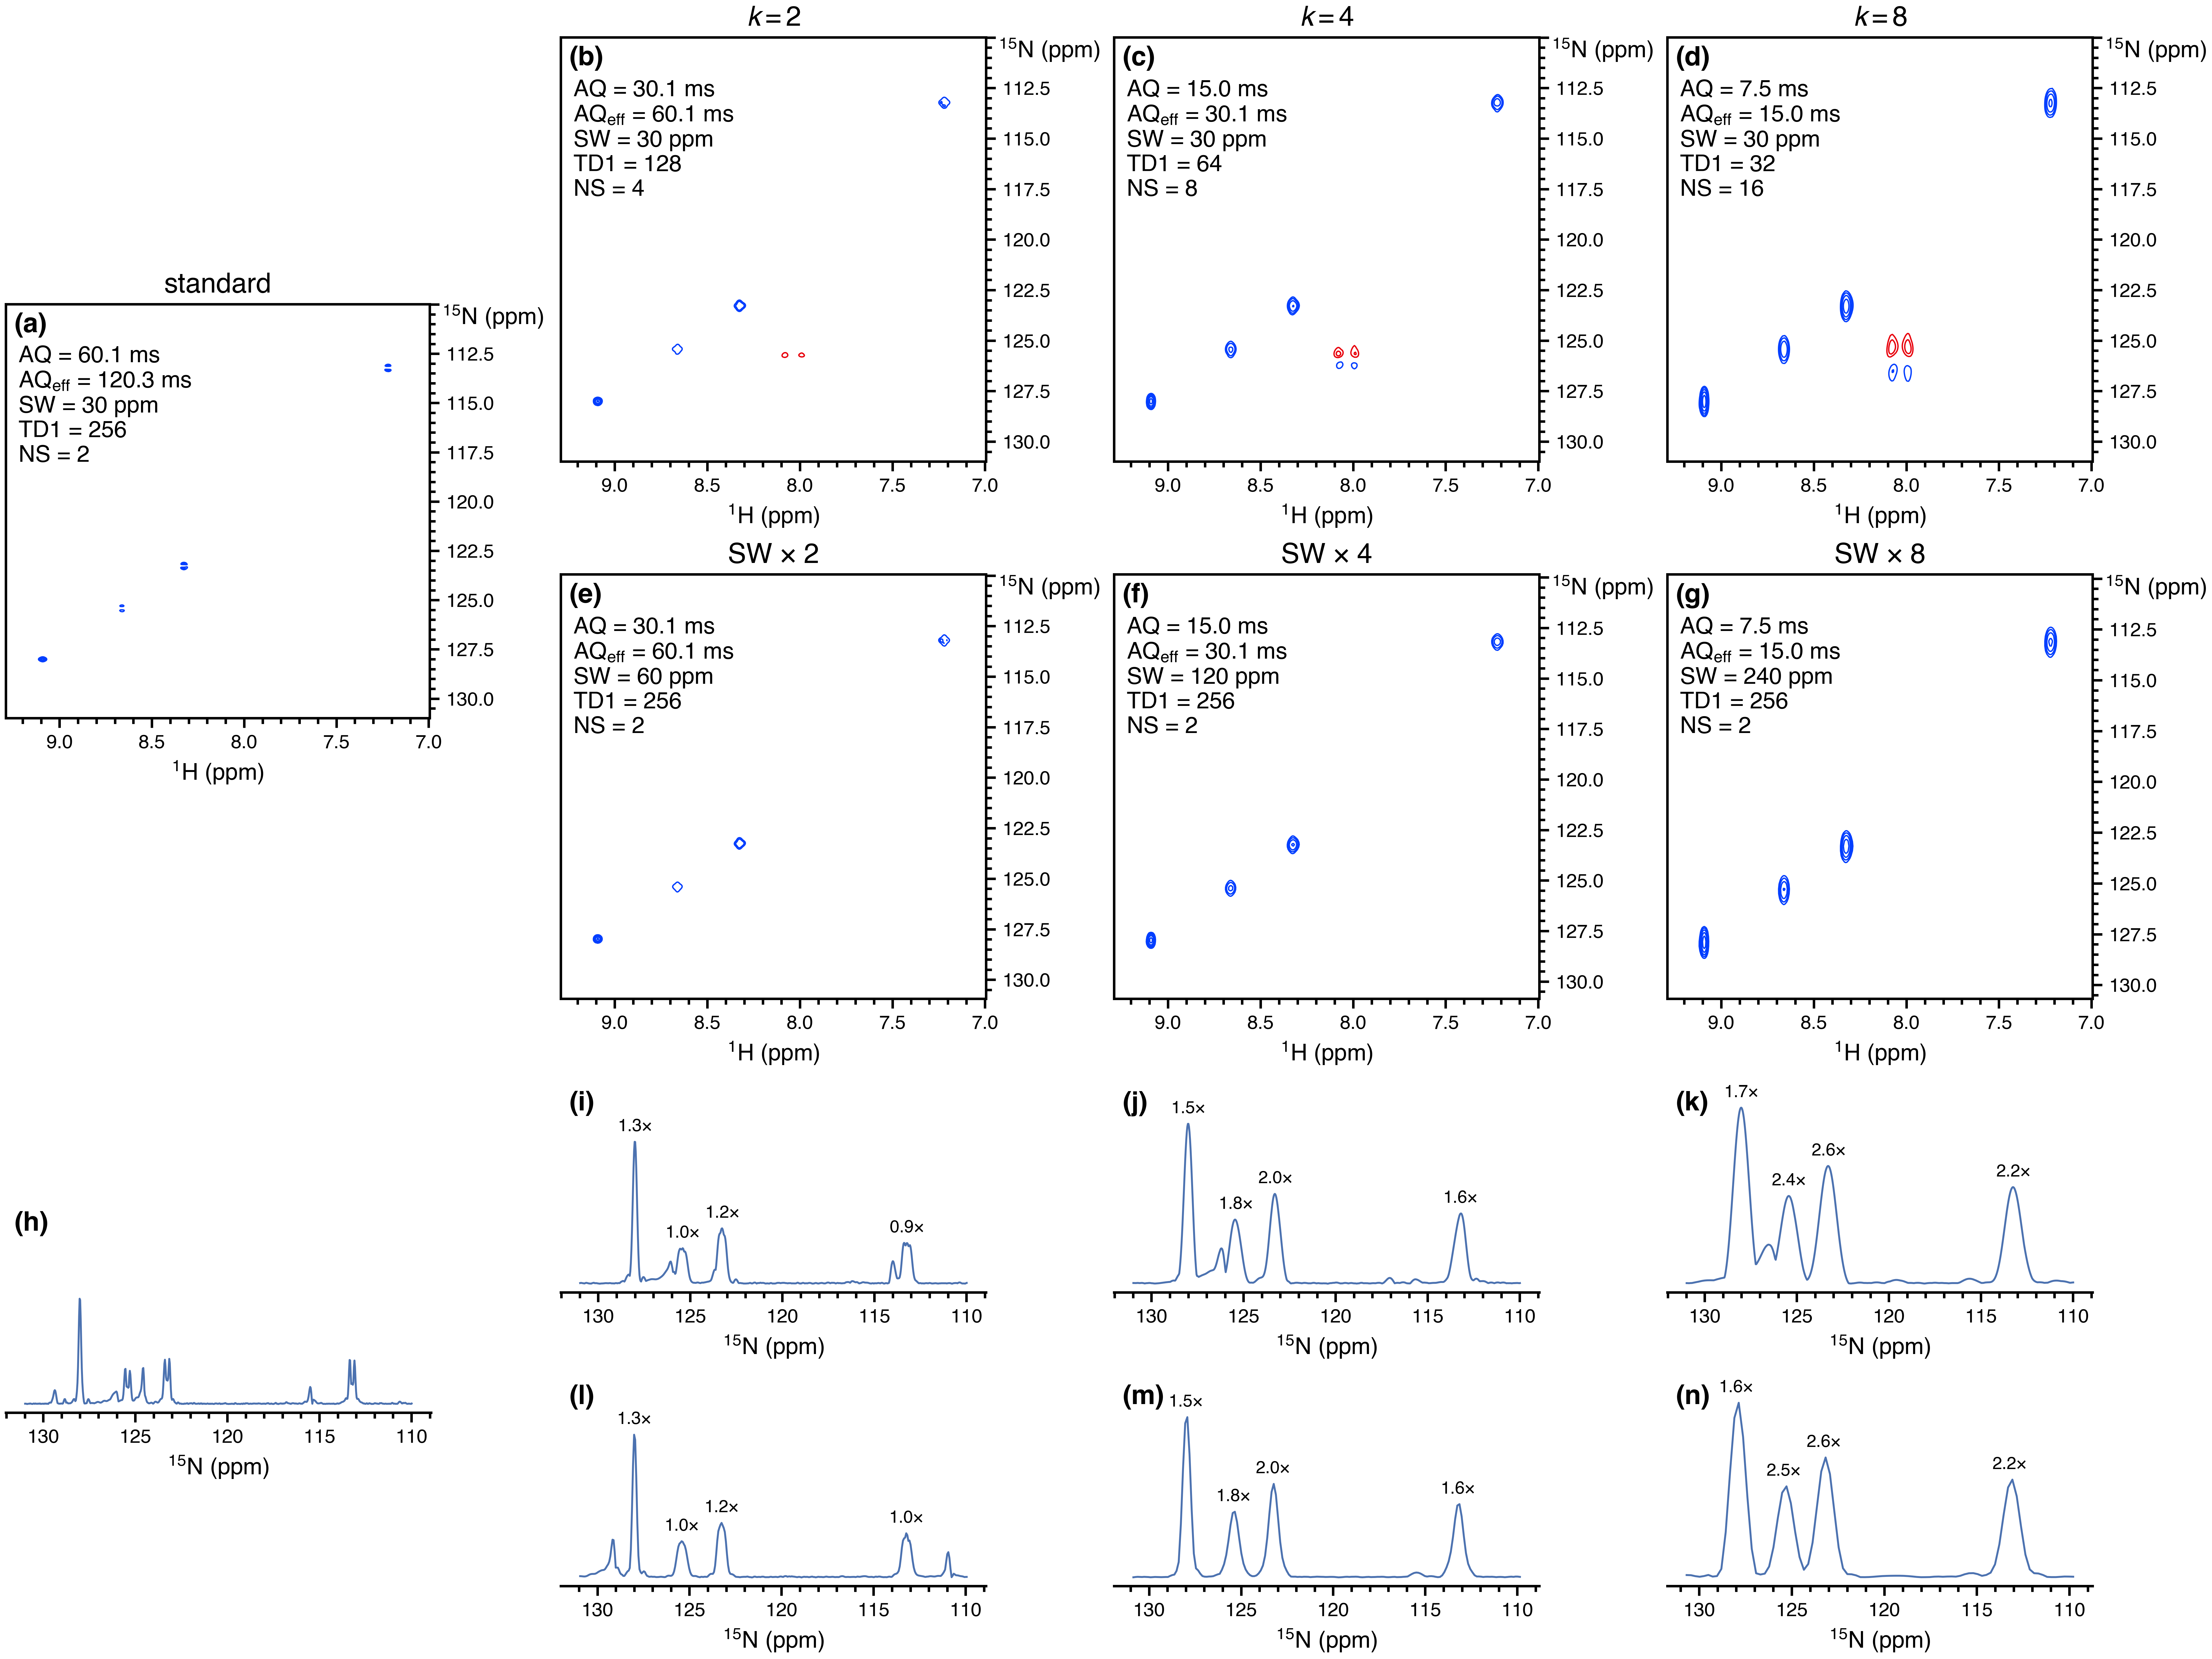
\includegraphics[width=0.75\textwidth]{./figures/hmqc_kscale.png}
    \caption{
        \textbf{(HMQC without linear prediction.)}
        \nitrogen{} HMQC spectra (from NOAH-3 \noahthree{M}{Sp}{Cc} supersequences) obtained with various values of the scaling factor $k$.
        The peak at $\delta_{\ce{H}} = \SI{8.03}{\ppm}$ is a folded peak from the ornithine \textdelta-\ce{NH2}.
        \textbf{(a)} $k = 1$, with 256 $t_1$ increments and 2 scans per increment (denoted as $256:2$).
        \textbf{(b)} $k = 2$, i.e.\ effectively 128 $t_1$ increments and 4 scans per increment ($128:4$).
        \textbf{(c)} $k = 4$ ($64:8$).
        \textbf{(d)} $k = 8$ ($32:16$).
        \textbf{(e)--(h)} Projections of 2D spectra in (a)--(d) onto the $f_1$ axis, shown at the same noise level.
        Numbers indicate peak heights relative to the $k = 1$ HMQC spectrum.
        \grami{}
    }
    \label{fig:hmqc_kscale}
\end{figure}

\begin{figure}
    \centering
    % figures/spv2_kscale.py
    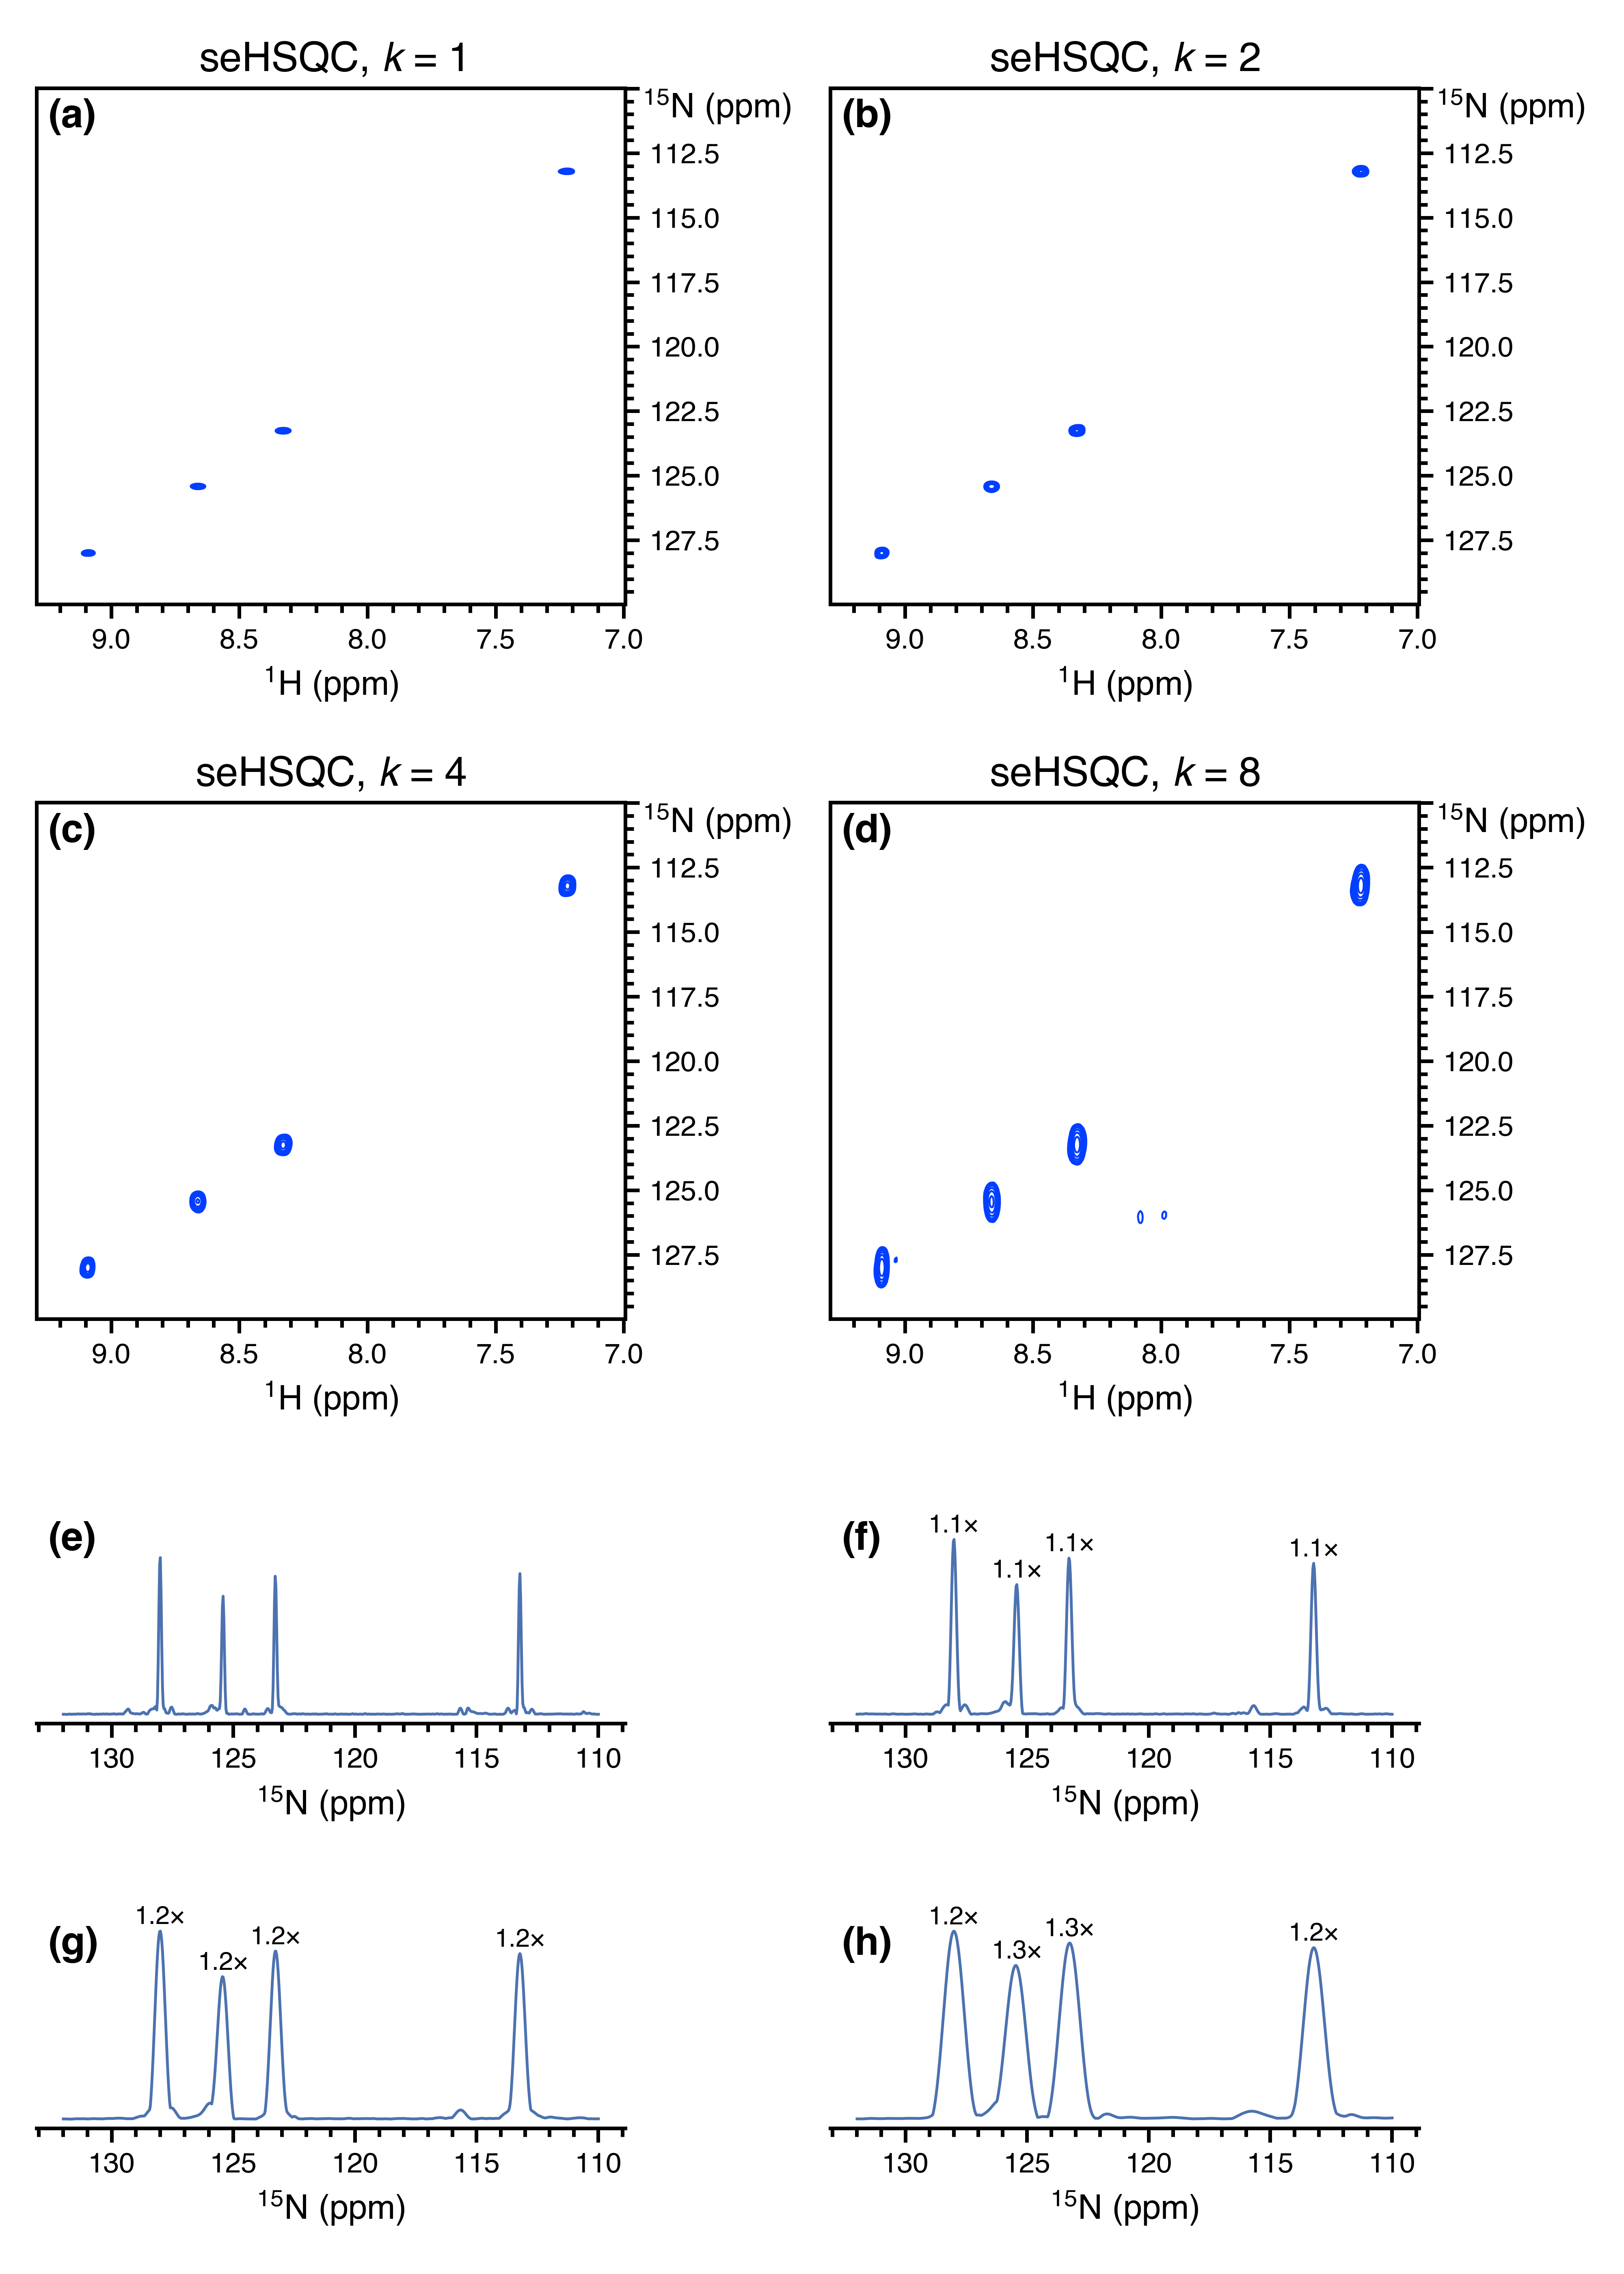
\includegraphics[width=0.75\textwidth]{./figures/spv2_kscale.png}
    \caption{
        \textbf{(seHSQC without linear prediction.)}
        \nitrogen{} seHSQC spectra (from NOAH-3 \noahthree{Spn}{Sp}{Cc} supersequences) obtained with various values of the scaling factor $k$.
        The peak at $\delta_{\ce{H}} = \SI{8.03}{\ppm}$ is a folded peak from the ornithine \textdelta-\ce{NH2}.
        \textbf{(a)} $k = 1$ (256 $t_1$ increments, 2 scans each).
        \textbf{(b)} $k = 2$ ($128:4$).
        \textbf{(c)} $k = 4$ ($64:8$).
        \textbf{(d)} $k = 8$ ($32:16$).
        \textbf{(e)--(h)} Projections of 2D spectra in (a)--(d) onto the $f_1$ axis, shown at the same noise level.
        Numbers indicate peak heights relative to the $k = 1$ seHSQC spectrum.
        \grami{}
    }
    \label{fig:spv2_kscale}
\end{figure}

\begin{figure}
    \centering
    % figures/hmqc_kscale_lp.py
    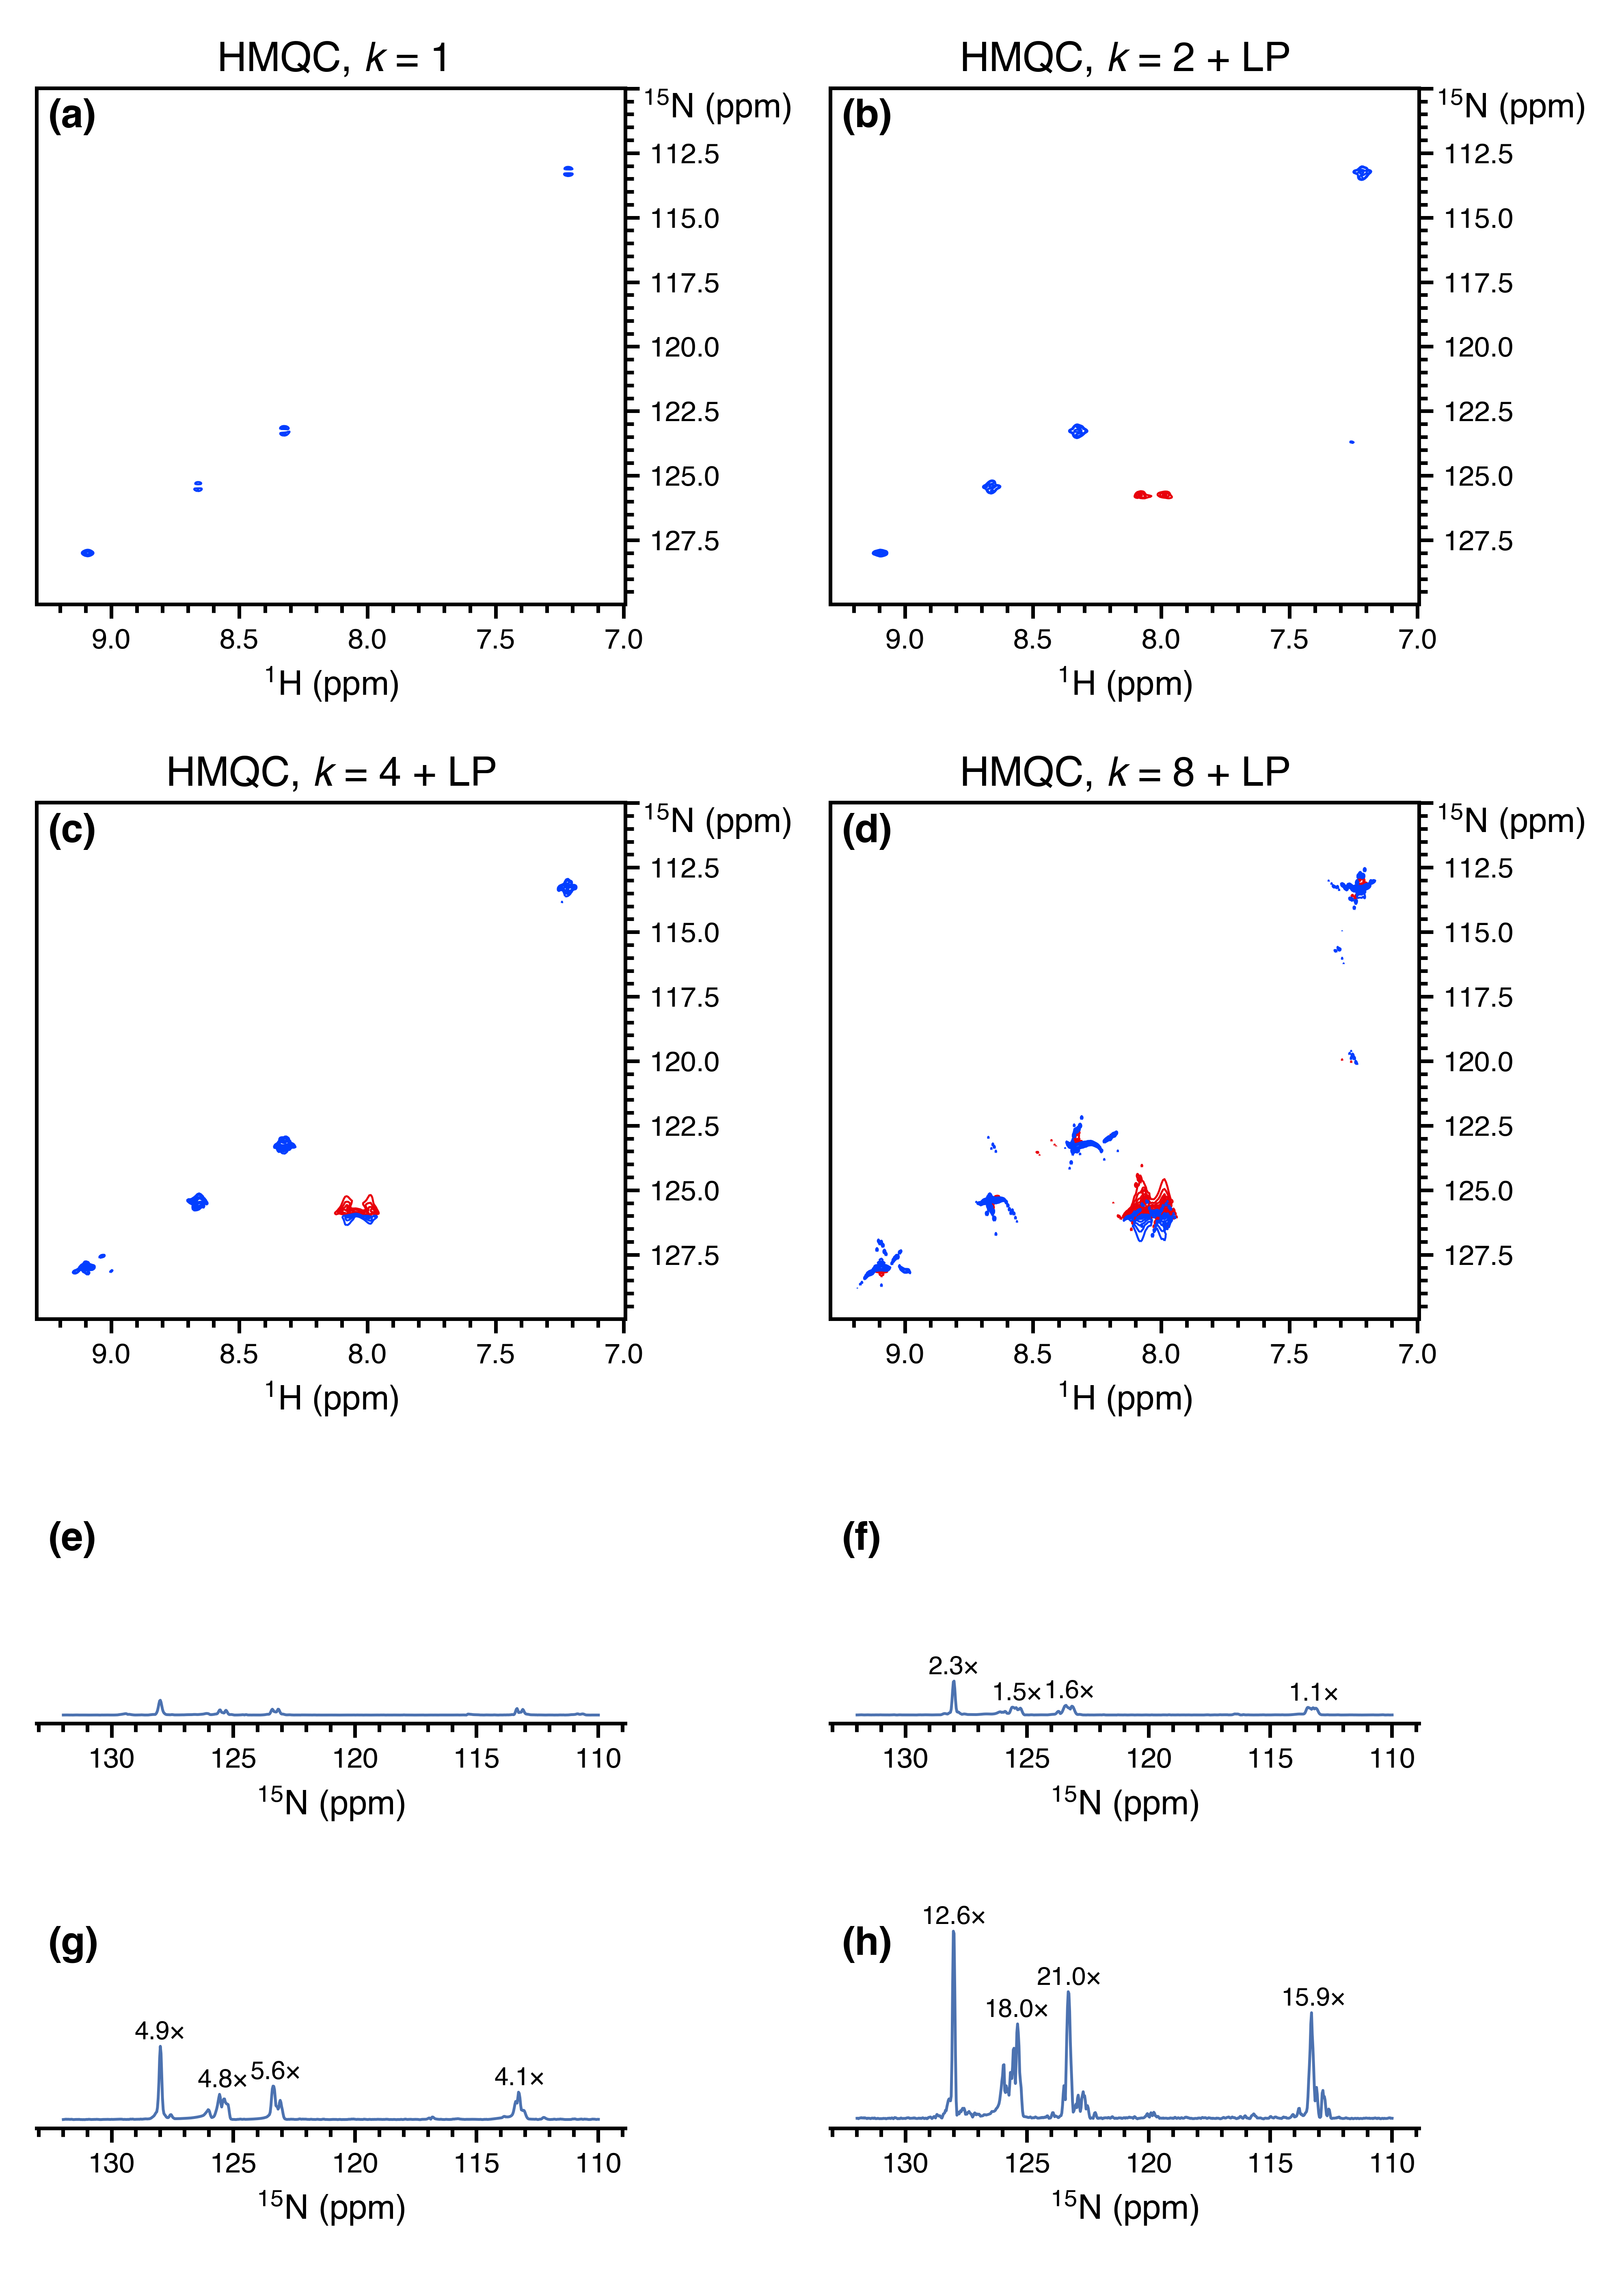
\includegraphics[width=0.75\textwidth]{./figures/hmqc_kscale_lp.png}
    \caption{
        \textbf{(HMQC with linear prediction.)}
        \nitrogen{} HMQC spectra (from NOAH-3 \noahthree{M}{Sp}{Cc} supersequences) obtained with various values of the scaling factor $k$, after linear prediction up to 512 complex points in $f_1$.
        The peak at $\delta_{\ce{H}} = \SI{8.03}{\ppm}$ is a folded peak from the ornithine \textdelta-\ce{NH2}.
        \textbf{(a)} $k = 1$ ($256:2$). Note that this spectrum is the same as in \figref{hmqc_kscale}a.
        \textbf{(b)} $k = 2$ ($128:4$).
        \textbf{(c)} $k = 4$ ($64:8$).
        \textbf{(d)} $k = 8$ ($32:16$).
        \textbf{(e)--(h)} Projections of 2D spectra in (a)--(d) onto the $f_1$ axis, shown at the same noise level.
        Numbers indicate peak heights relative to the $k = 1$ HMQC spectrum.
        \grami{}
    }
    \label{fig:hmqc_kscale_lp}
\end{figure}

\begin{figure}
    \centering
    % figures/spv2_kscale_lp.py
    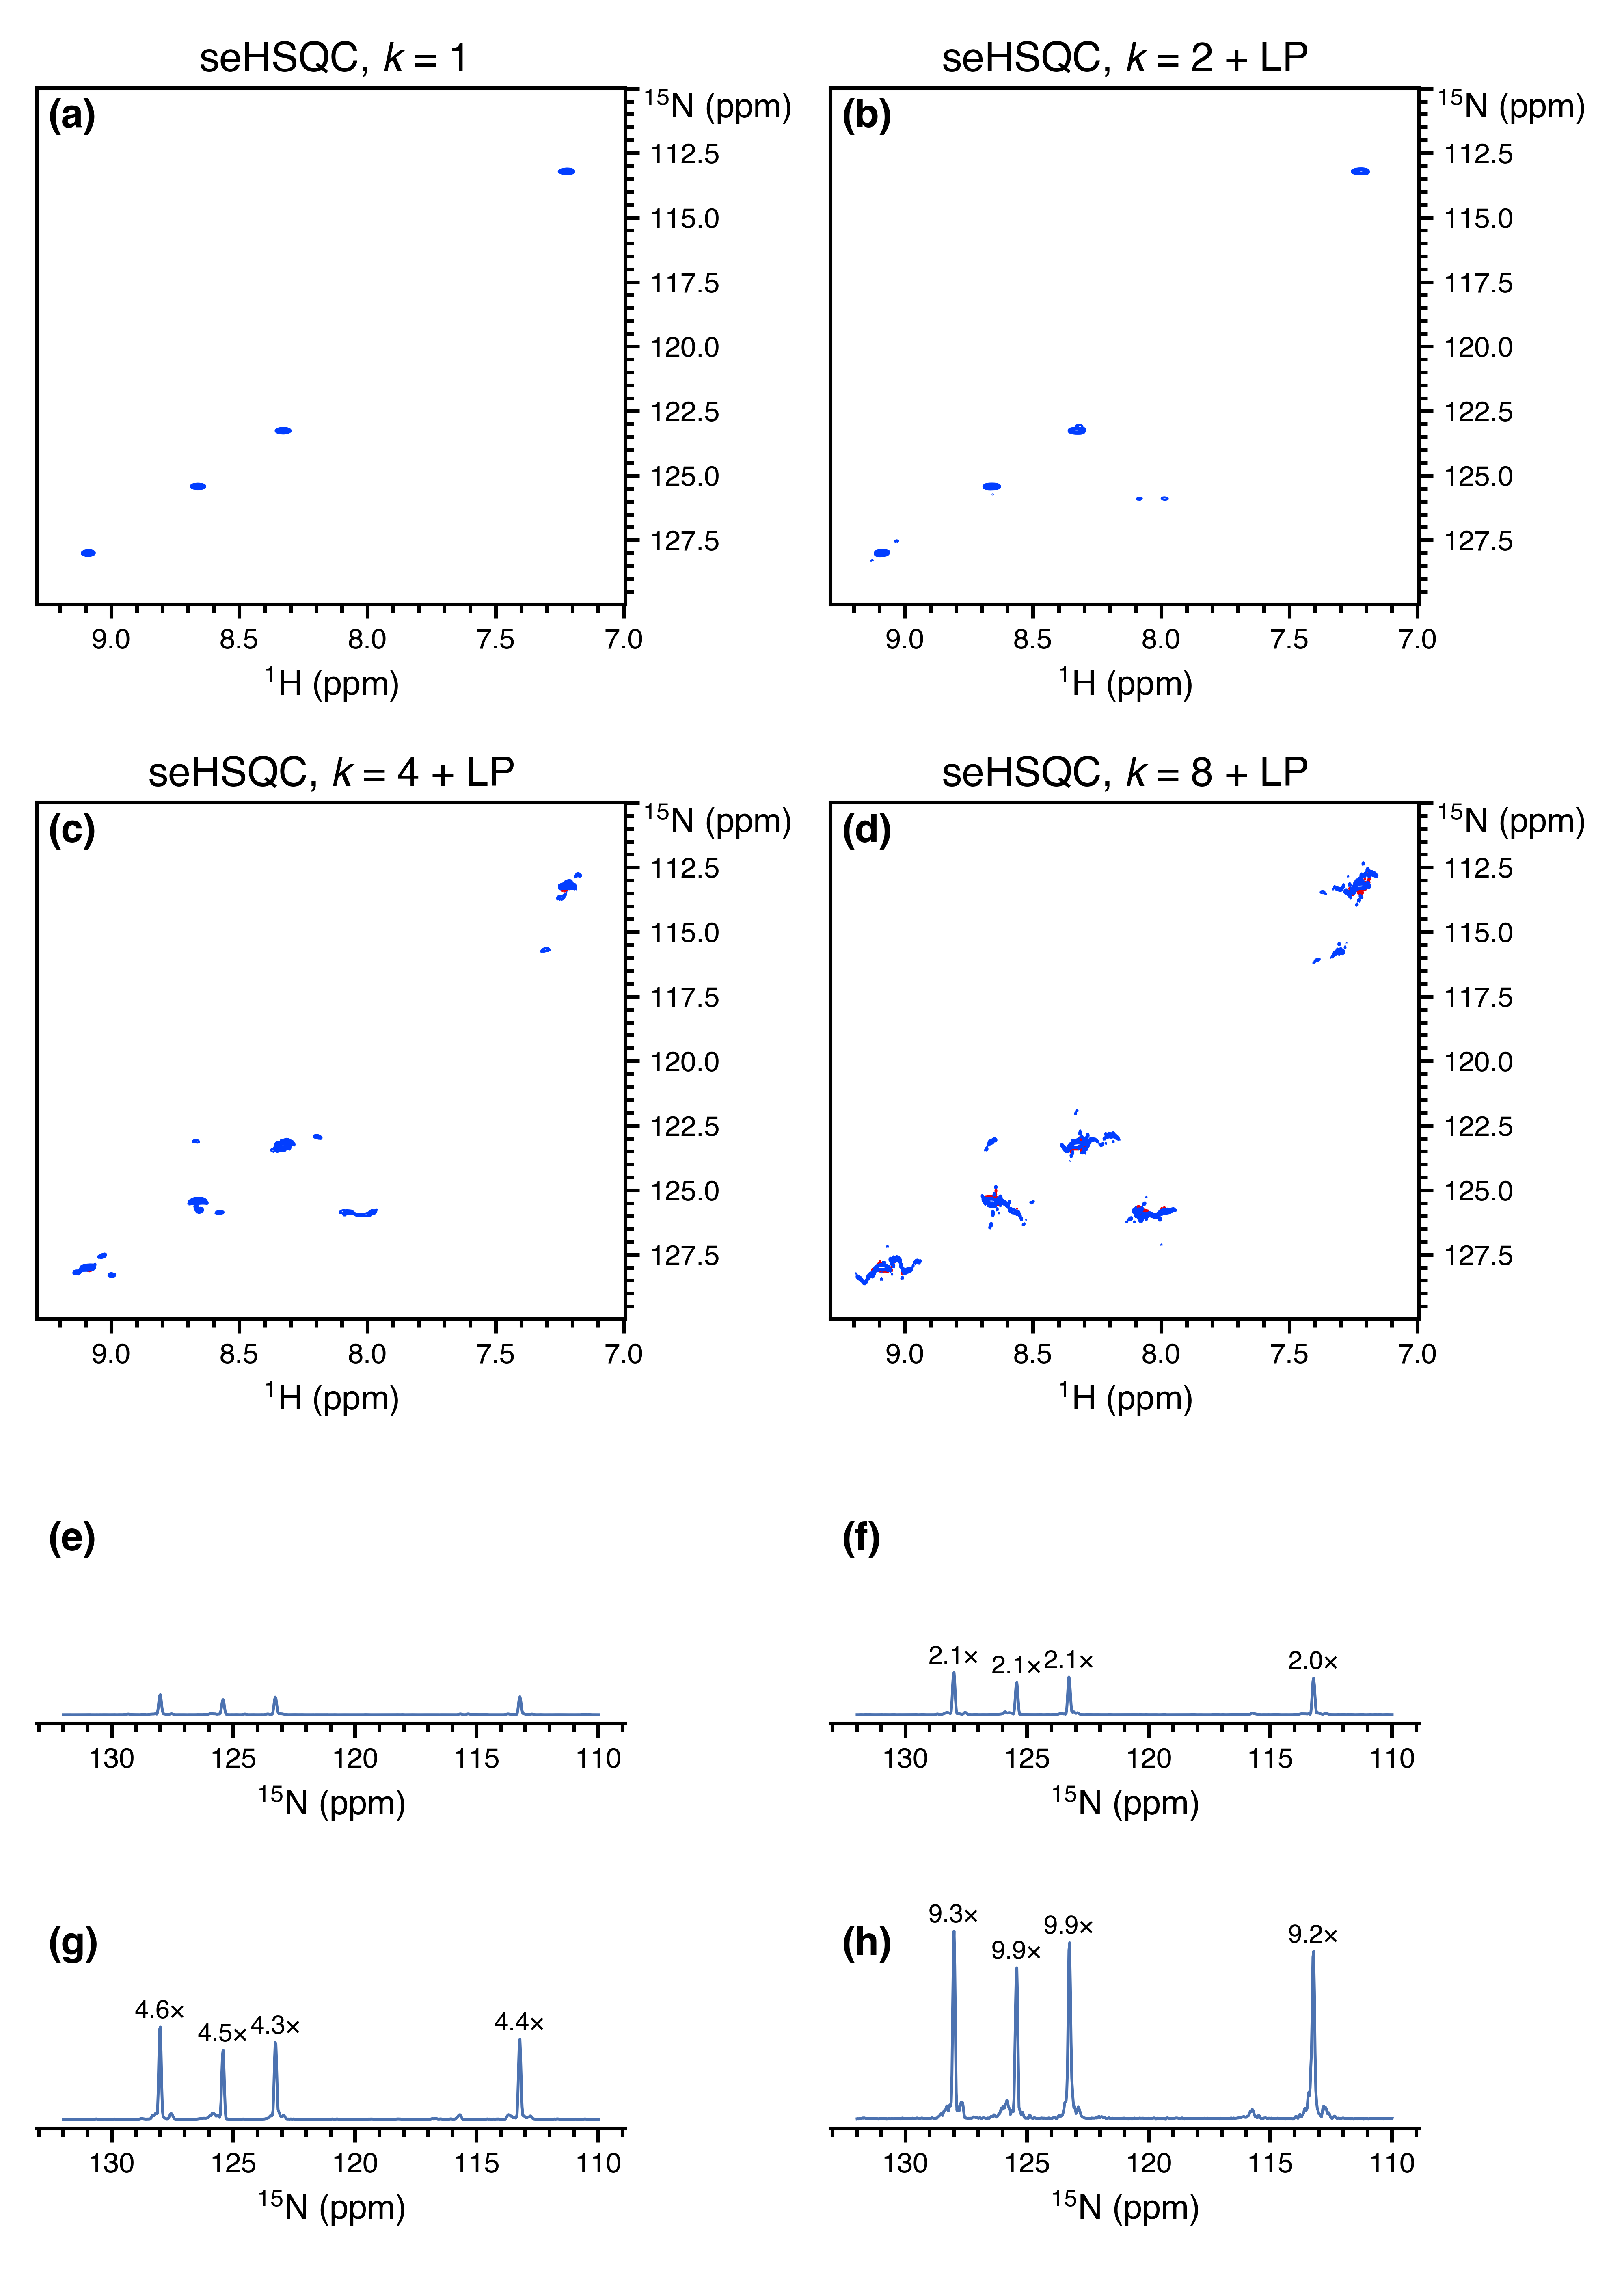
\includegraphics[width=0.75\textwidth]{./figures/spv2_kscale_lp.png}
    \caption{
        \textbf{(seHSQC with linear prediction.)}
        \nitrogen{} seHSQC spectra (from NOAH-3 \noahthree{Spn}{Sp}{Cc} supersequences) obtained with various values of the scaling factor $k$, after linear prediction up to 512 complex points in $f_1$.
        The peak at $\delta_{\ce{H}} = \SI{8.03}{\ppm}$ is a folded peak from the ornithine \textdelta-\ce{NH2}.
        \textbf{(a)} $k = 1$ ($256:2$). Note that this spectrum is the same as in \figref{spv2_kscale}a.
        \textbf{(b)} $k = 2$ ($128:4$).
        \textbf{(c)} $k = 4$ ($64:8$).
        \textbf{(d)} $k = 8$ ($32:16$).
        \textbf{(e)--(h)} Projections of 2D spectra in (a)--(d) onto the $f_1$ axis, shown at the same noise level.
        Numbers indicate peak heights relative to the $k = 1$ seHSQC spectrum.
        \grami{}
    }
    \label{fig:spv2_kscale_lp}
\end{figure}

\section{HSQC-TOCSY/HSQC sensitivity comparisons}

The signal intensities for the NOAH-3 \noahthree{St}{S}{Cc} (HSQC-TOCSY + HSQC + CLIP-COSY) supersequences can be more conveniently measured by omitting the DIPSI-2 isotropic mixing in the HSQC-TOCSY supersequence, leading to a NOAH-3 \noahthree{S}{S}{Cc} (HSQC + HSQC + CLIP-COSY) supersequence.
This allows us to compare the different versions of double-HSQC sequences, as the two HSQC modules can be implemented either using the MFA approach, or the new ASAP/NOAH approach based on Ernst angle excitation in the first module.
In the latter implementation, the parameter $f$ can be varied between 0.4 and 1; it represents the proportion of \magn{\ce{C}} magnetisation used in the first HSQC, as described in the main text.
Furthermore, to boost the sensitivity of the second HSQC module in the NOAH supersequences, the new seHSQC module can be used in its place.

\begin{figure}
    \centering
    % figures/ssc_comparisons.py
    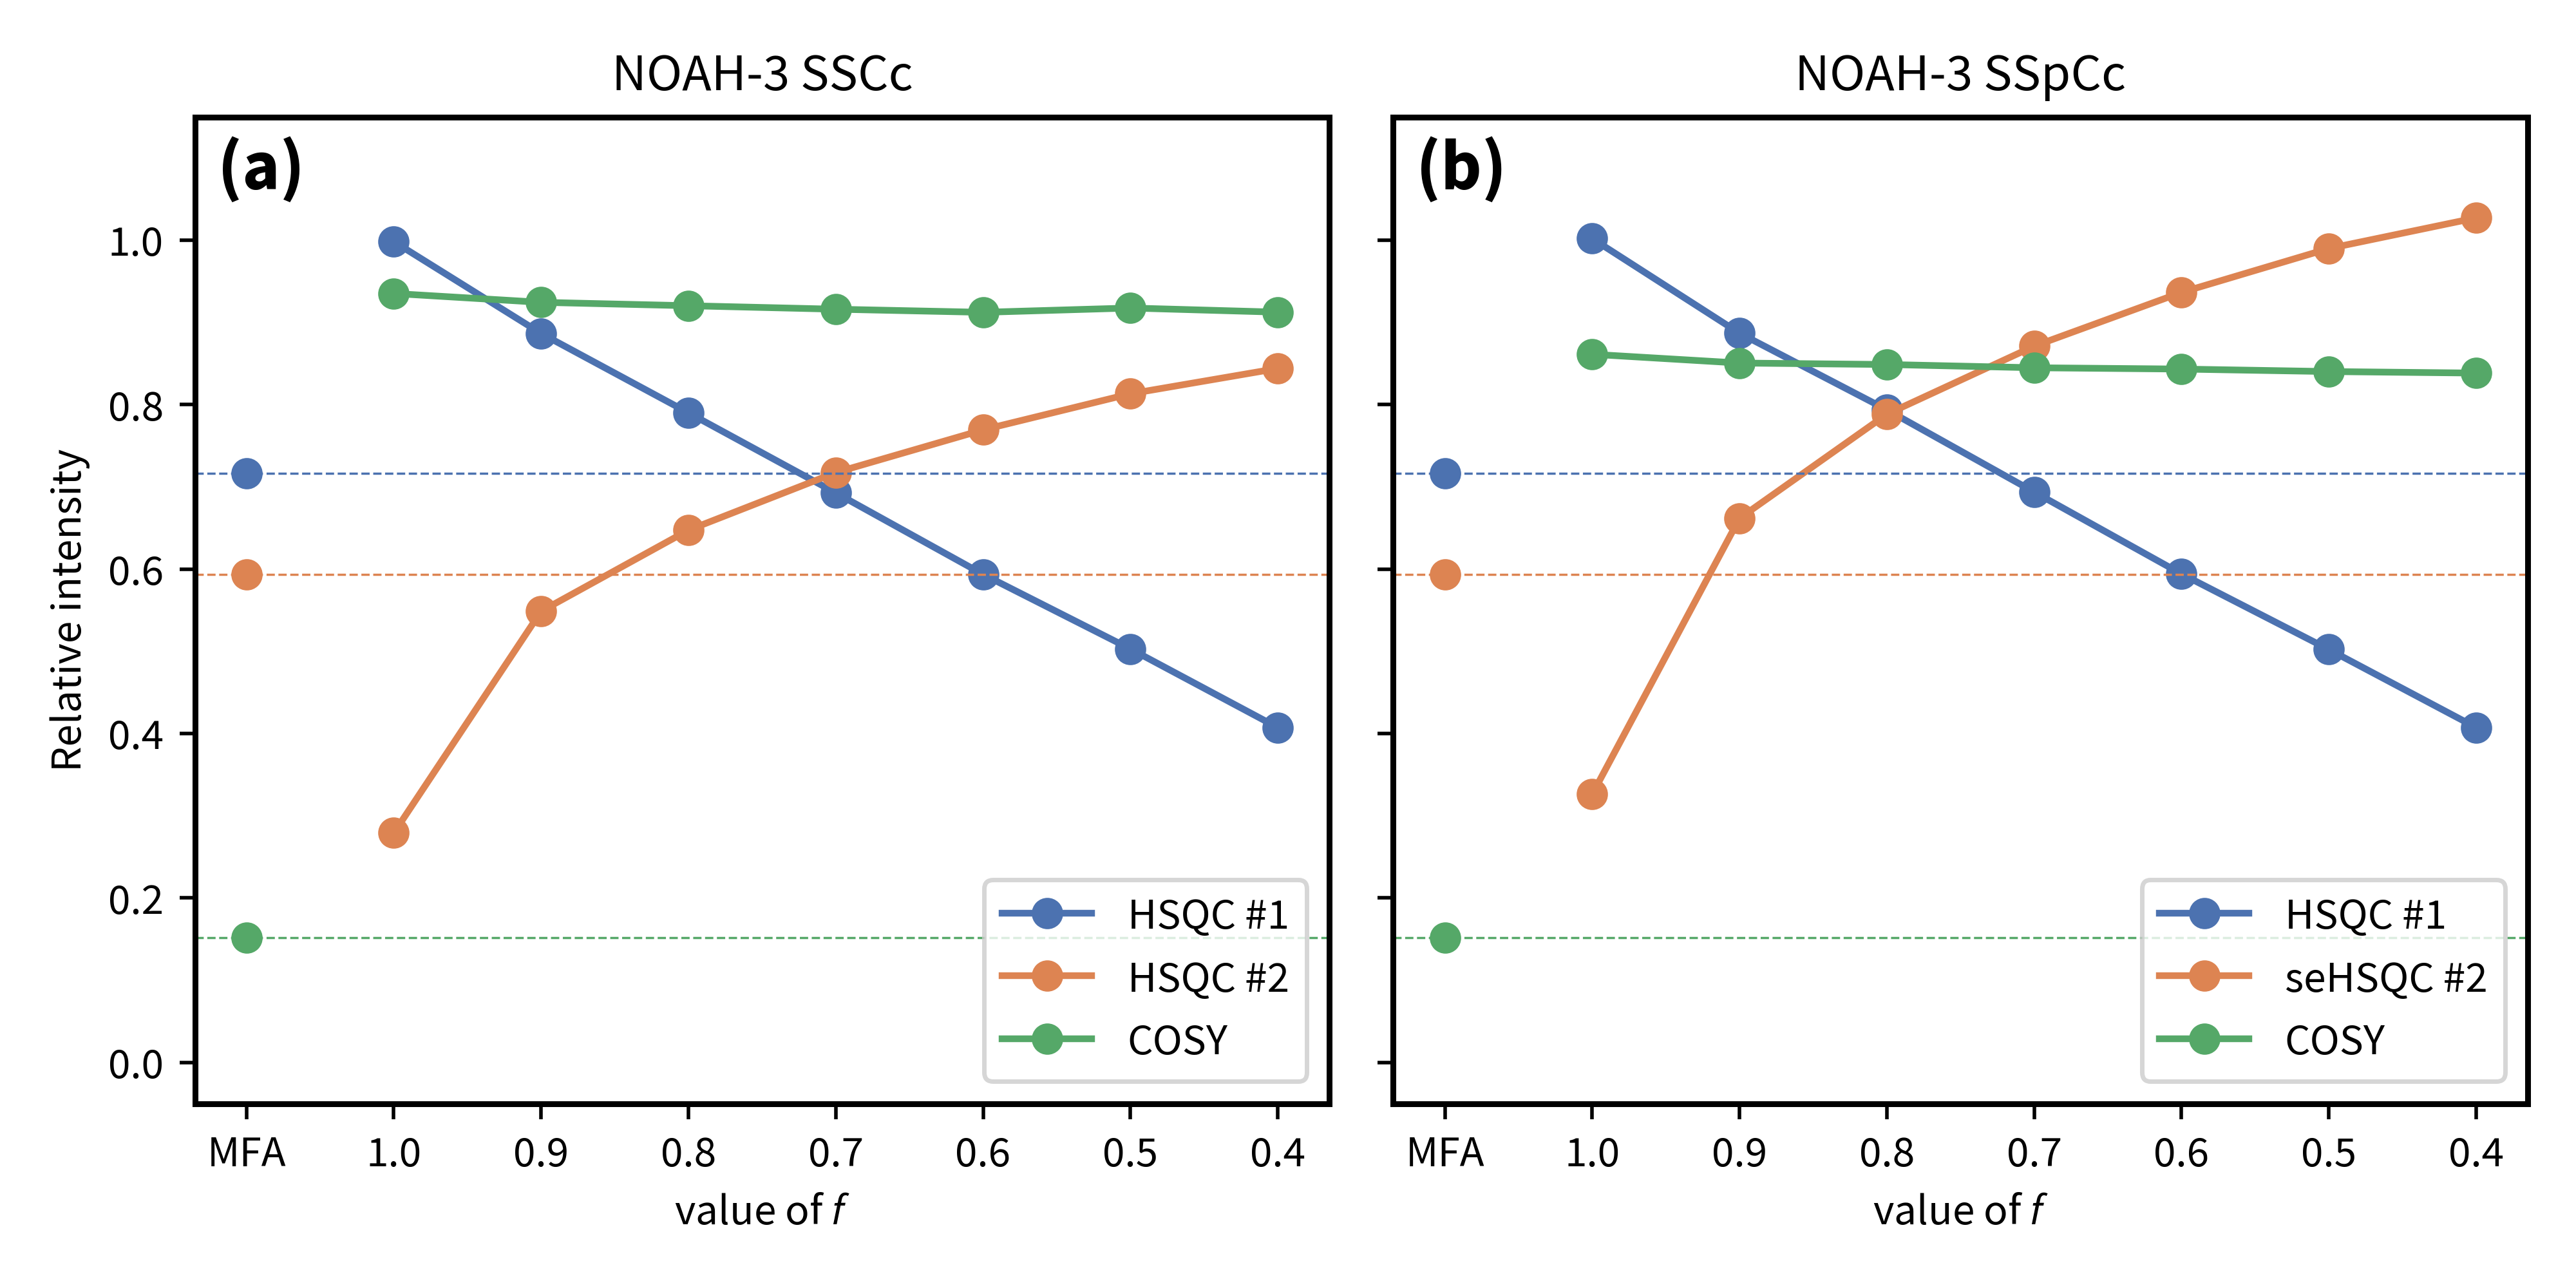
\includegraphics[width=0.8\textwidth]{./figures/ssc_comparisons.png}
    \caption{
        Sensitivities of HSQC and CLIP-COSY modules when used as part of a \noahthree{S}{S}{Cc}-type supersequence, with both the NOAH and MFA implementations of the two HSQC modules.
        Intensities are calculated relative to the HSQC and CLIP-COSY modules in a standard NOAH-2 SCc supersequence (averaged over all peaks).
        \textbf{(a)} Sensitivity of the MFA implementation (i.e.\ a MFA double HSQC experiment immediately followed by a CLIP-COSY).
        Horizontal dashed lines at these levels are drawn across all subplots to guide the eye.
        \textbf{(b)} Sensitivity of NOAH-3 \noahthree{S}{S}{Cc} modules as a function of $f$.
        Note that at $f = 0.8$, all of the NOAH spectra have a greater average sensitivity than their MFA counterparts.
        \textbf{(c)} Sensitivity of NOAH-3 \noahthree{S}{Sp}{Cc} modules as a function of $f$.
        \andro{}
    }
    \label{fig:ssc_comparisons}
\end{figure}

\figref{ssc_comparisons} may be understood in the following way:

\begin{itemize}
    \item The MFA HSQC sensitivities (in (a)) are approximately half that of a standard CRK seHSQC, with the second HSQC having slightly lower sensitivity.
        This is discussed in ref.\ \citenum{Nolis2019CPC} of the main text.
    \item The sensitivity of the first NOAH HSQC (blue in (b) and (c)) is generally equal to $f$, supporting the interpretation of $f$ as the fraction of \carbon{}--\proton{} magnetisation excited in the first HSQC.
    \item The sensitivity of the second NOAH HSQC (orange in (b)) arises from whatever is \textit{not} used by the first HSQC, plus any magnetisation that relaxes during the FID of the first HSQC.
        As $f$ is decreased, the former contribution increases and the latter tapers off.
        This is true for the seHSQC as well (orange in (c)), except that there is a uniform boost in sensitivity for all values of $f$.
        This sensitivity improvement mainly applies to \ce{CH} groups, as discussed in the main text.
    \item The MFA COSY sensitivity (green) is substantially lower ($\sim 15\%$) because the bulk magnetisation is dephased by the previous modules, whereas in the NOAH approach it is (largely) preserved.
\end{itemize}

It remains to evaluate the impact of adding DIPSI-2 mixing in one of the HSQC modules on the remaining modules in the supersequence.
This depends on whether the HSQC-TOCSY module is placed first (\noahthree{St}{S}{Cc} or \noahthree{St}{Sp}{Cc}) or second (\noahthree{S}{St}{Cc}) in the sequence.
Since the seHSQC module does not preserve unused \magn{\ce{C}} magnetisation, the HSQC-TOCSY in a hypothetical \noahthree{Sp}{St}{Cc} supersequence will have greatly reduced sensitivity.
On the other hand, placing the HSQC-TOCSY sequence first allows the seHSQC module to be used subsequent to this; we therefore consider only the permutations where the HSQC-TOCSY goes first.

\begin{figure}
    \centering
    % figures/stsc_comparisons.py
    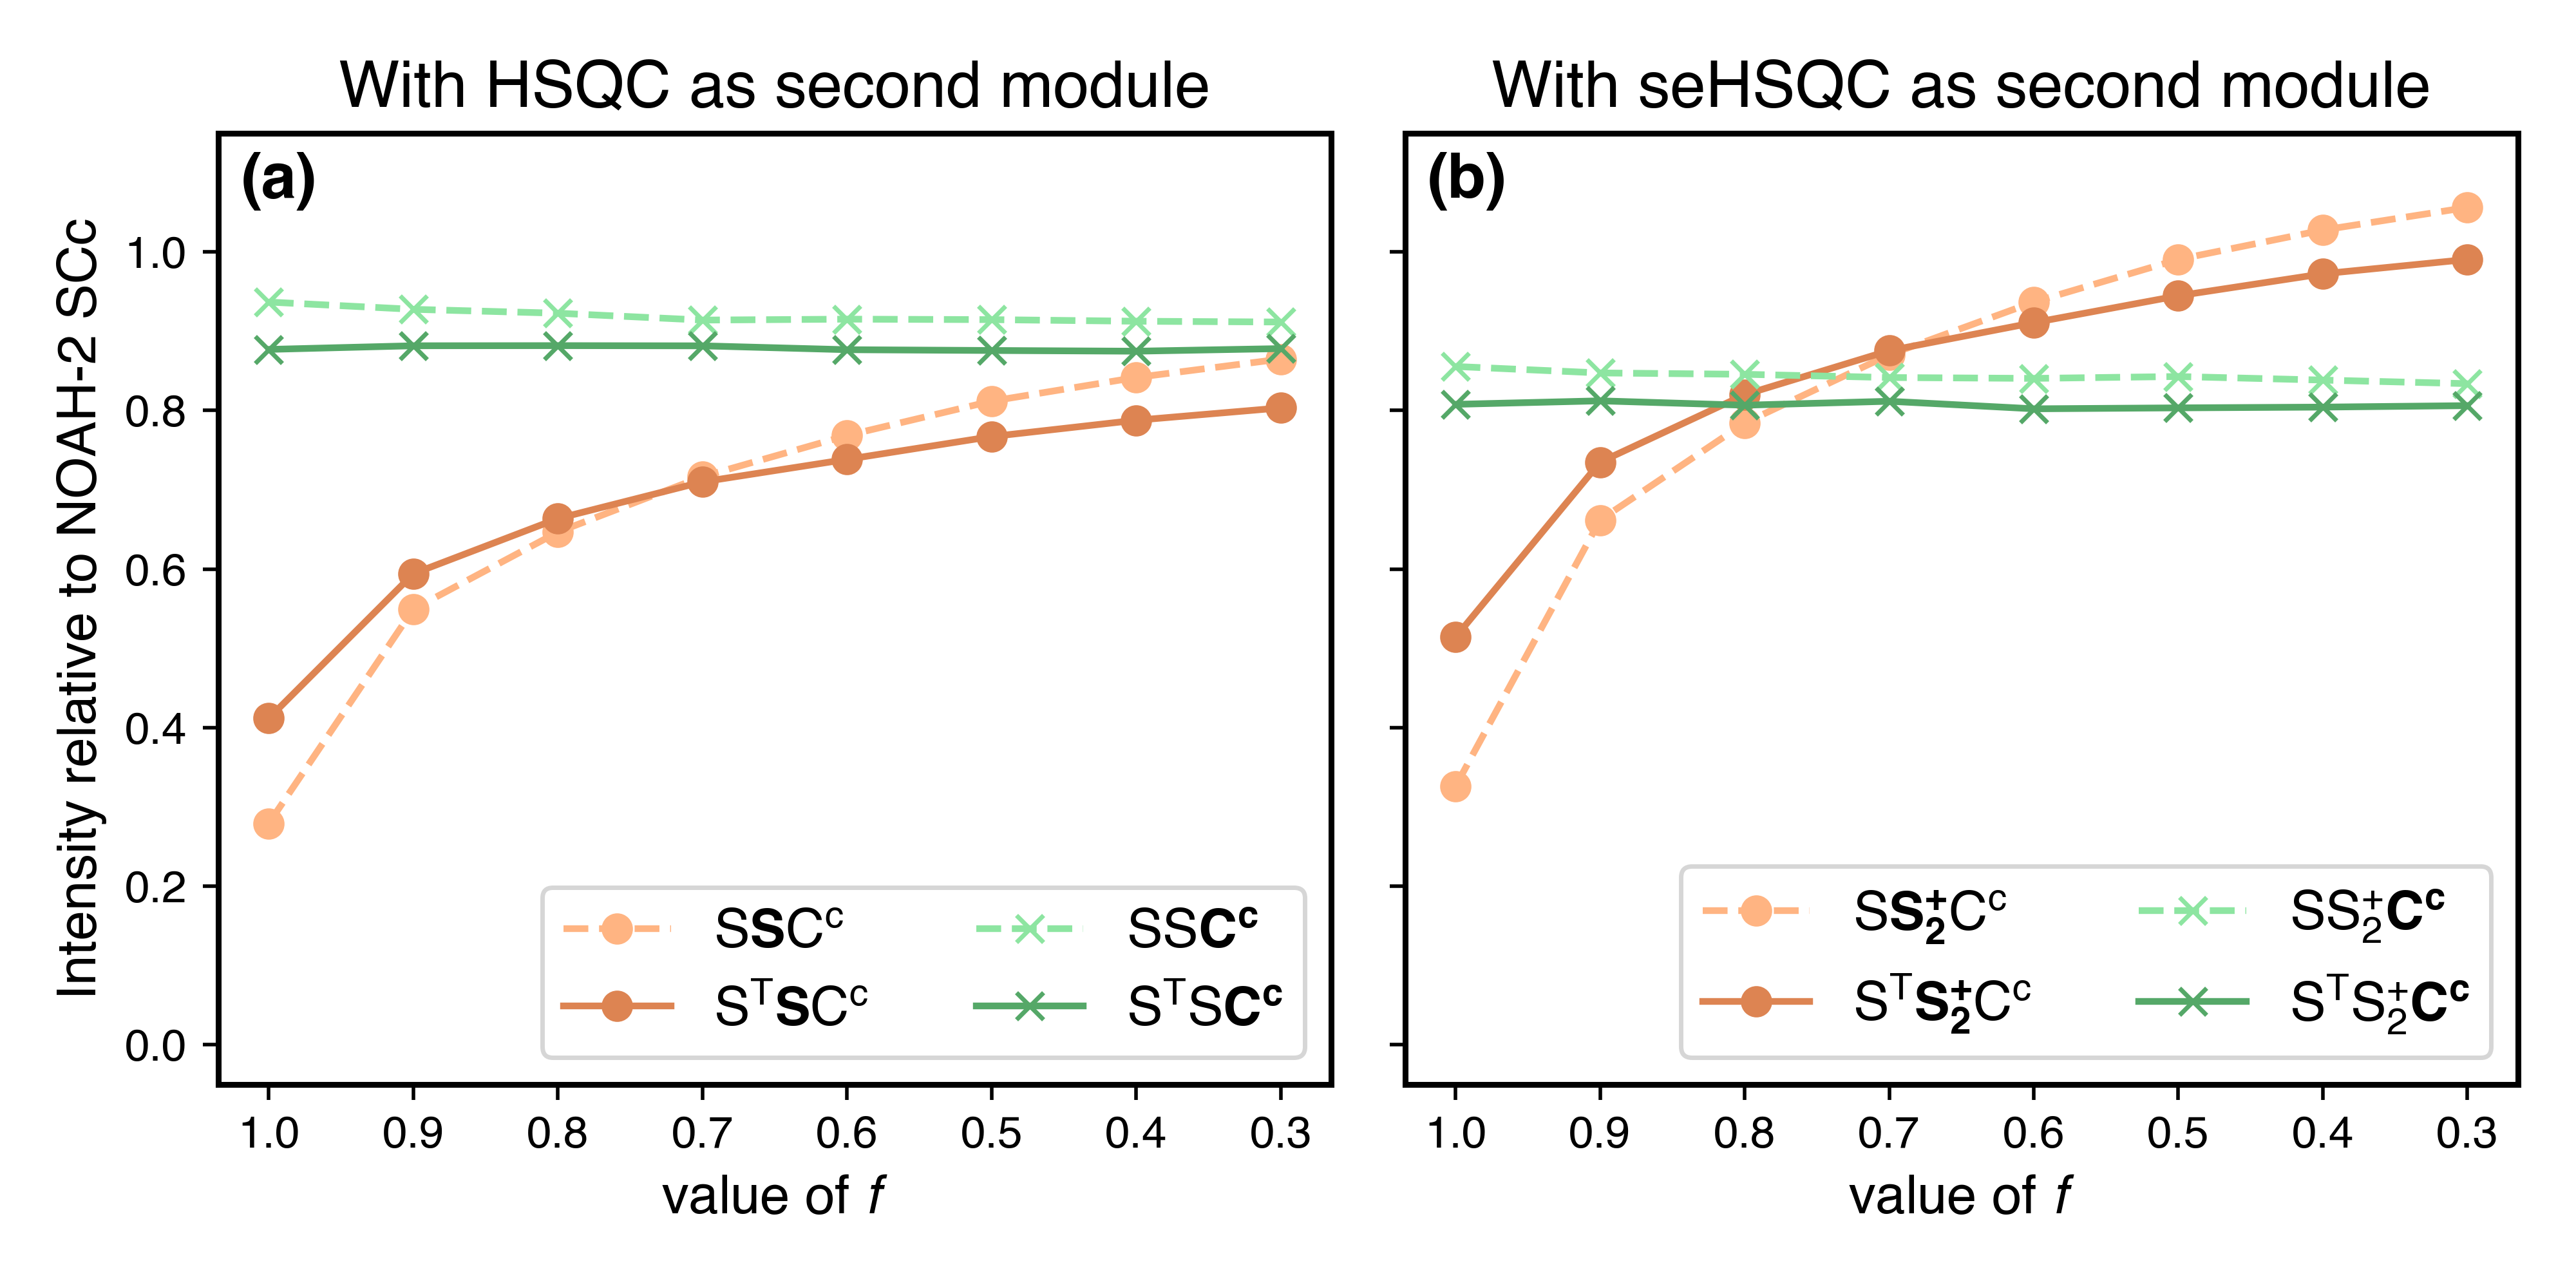
\includegraphics[width=0.8\textwidth]{./figures/stsc_comparisons.png}
    \caption{
        Comparison of signal intensities of second (HSQC or seHSQC) and third (CLIP-COSY) modules in the \noahthree{St}{S}{Cc} and \noahthree{St}{Sp}{Cc} supersequences, versus their intensities in the \noahthree{S}{S}{Cc} and \noahthree{S}{Sp}{Cc} sequences, as a function of the parameter $f$.
        The solid, darker lines indicate the supersequences beginning with the HSQC-TOCSY, whereas the dashed, lighter lines indicate the supersequences beginning with the HSQC (the latter are the same graphs as in \figref{ssc_comparisons}).
        \textbf{(a)} With the HSQC as the second module.
        \textbf{(b)} With the seHSQC as the second module.
        \andro{}
    }
    \label{fig:stsc_comparisons}
\end{figure}

It can be seen from \figref{stsc_comparisons} that the introduction of DIPSI-2 mixing leads to a very small drop ($< 10\%$) in the amount of \magnnot{\ce{C}} magnetisation preserved for the COSY module.
On the other hand, the HSQC (and seHSQC) sensitivites follow largely the same trend as before.
For values of $f$ above $0.7$ (where relatively little \magn{\ce{C}} magnetisation is preserved for these modules), the DIPSI-2 mixing helps to replenish some of this magnetisation.
As $f$ decreases, this effect becomes smaller, and at small $f$ it even leads to a reduction in signal intensity.
As discussed in the main text, since the HSQC-TOCSY has a lower intrinsic sensitivity than the (se)HSQC, we recommend using a large value of $f$, such as $0.9$.
This does not compromise the HSQC-TOCSY intensity by much, and at the same time yields either a HSQC with $\sim 65\%$ of its original sensitivity, or a seHSQC which has $\sim 80\%$ of the sensitivity of a standard NOAH HSQC.

Finally, we note that because a significant proportion of the HSQC signal derives from \magn{\ce{C}} relaxation during the HSQC-TOCSY FID, use of a larger acquisition time (AQ) can potentially boost the HSQC sensitivity even further.
The experiments shown above were carried out with a relatively short AQ of \SI{73}{\ms}.
\textbf{However, bear in mind that the high duty cycle associated with broadband \ce{^13C} decoupling can potentially cause hardware damage if applied for too long, especially given that the supersequences described here have two consecutive \ce{^13C}-decoupled modules.}

\section{Other example spectra}
\label{section:si_spectra}

\begin{figure}
    \centering
    % figures/stspct.py
    
\includegraphics{./figures/andro.png}\phantom{aaaaaa}
    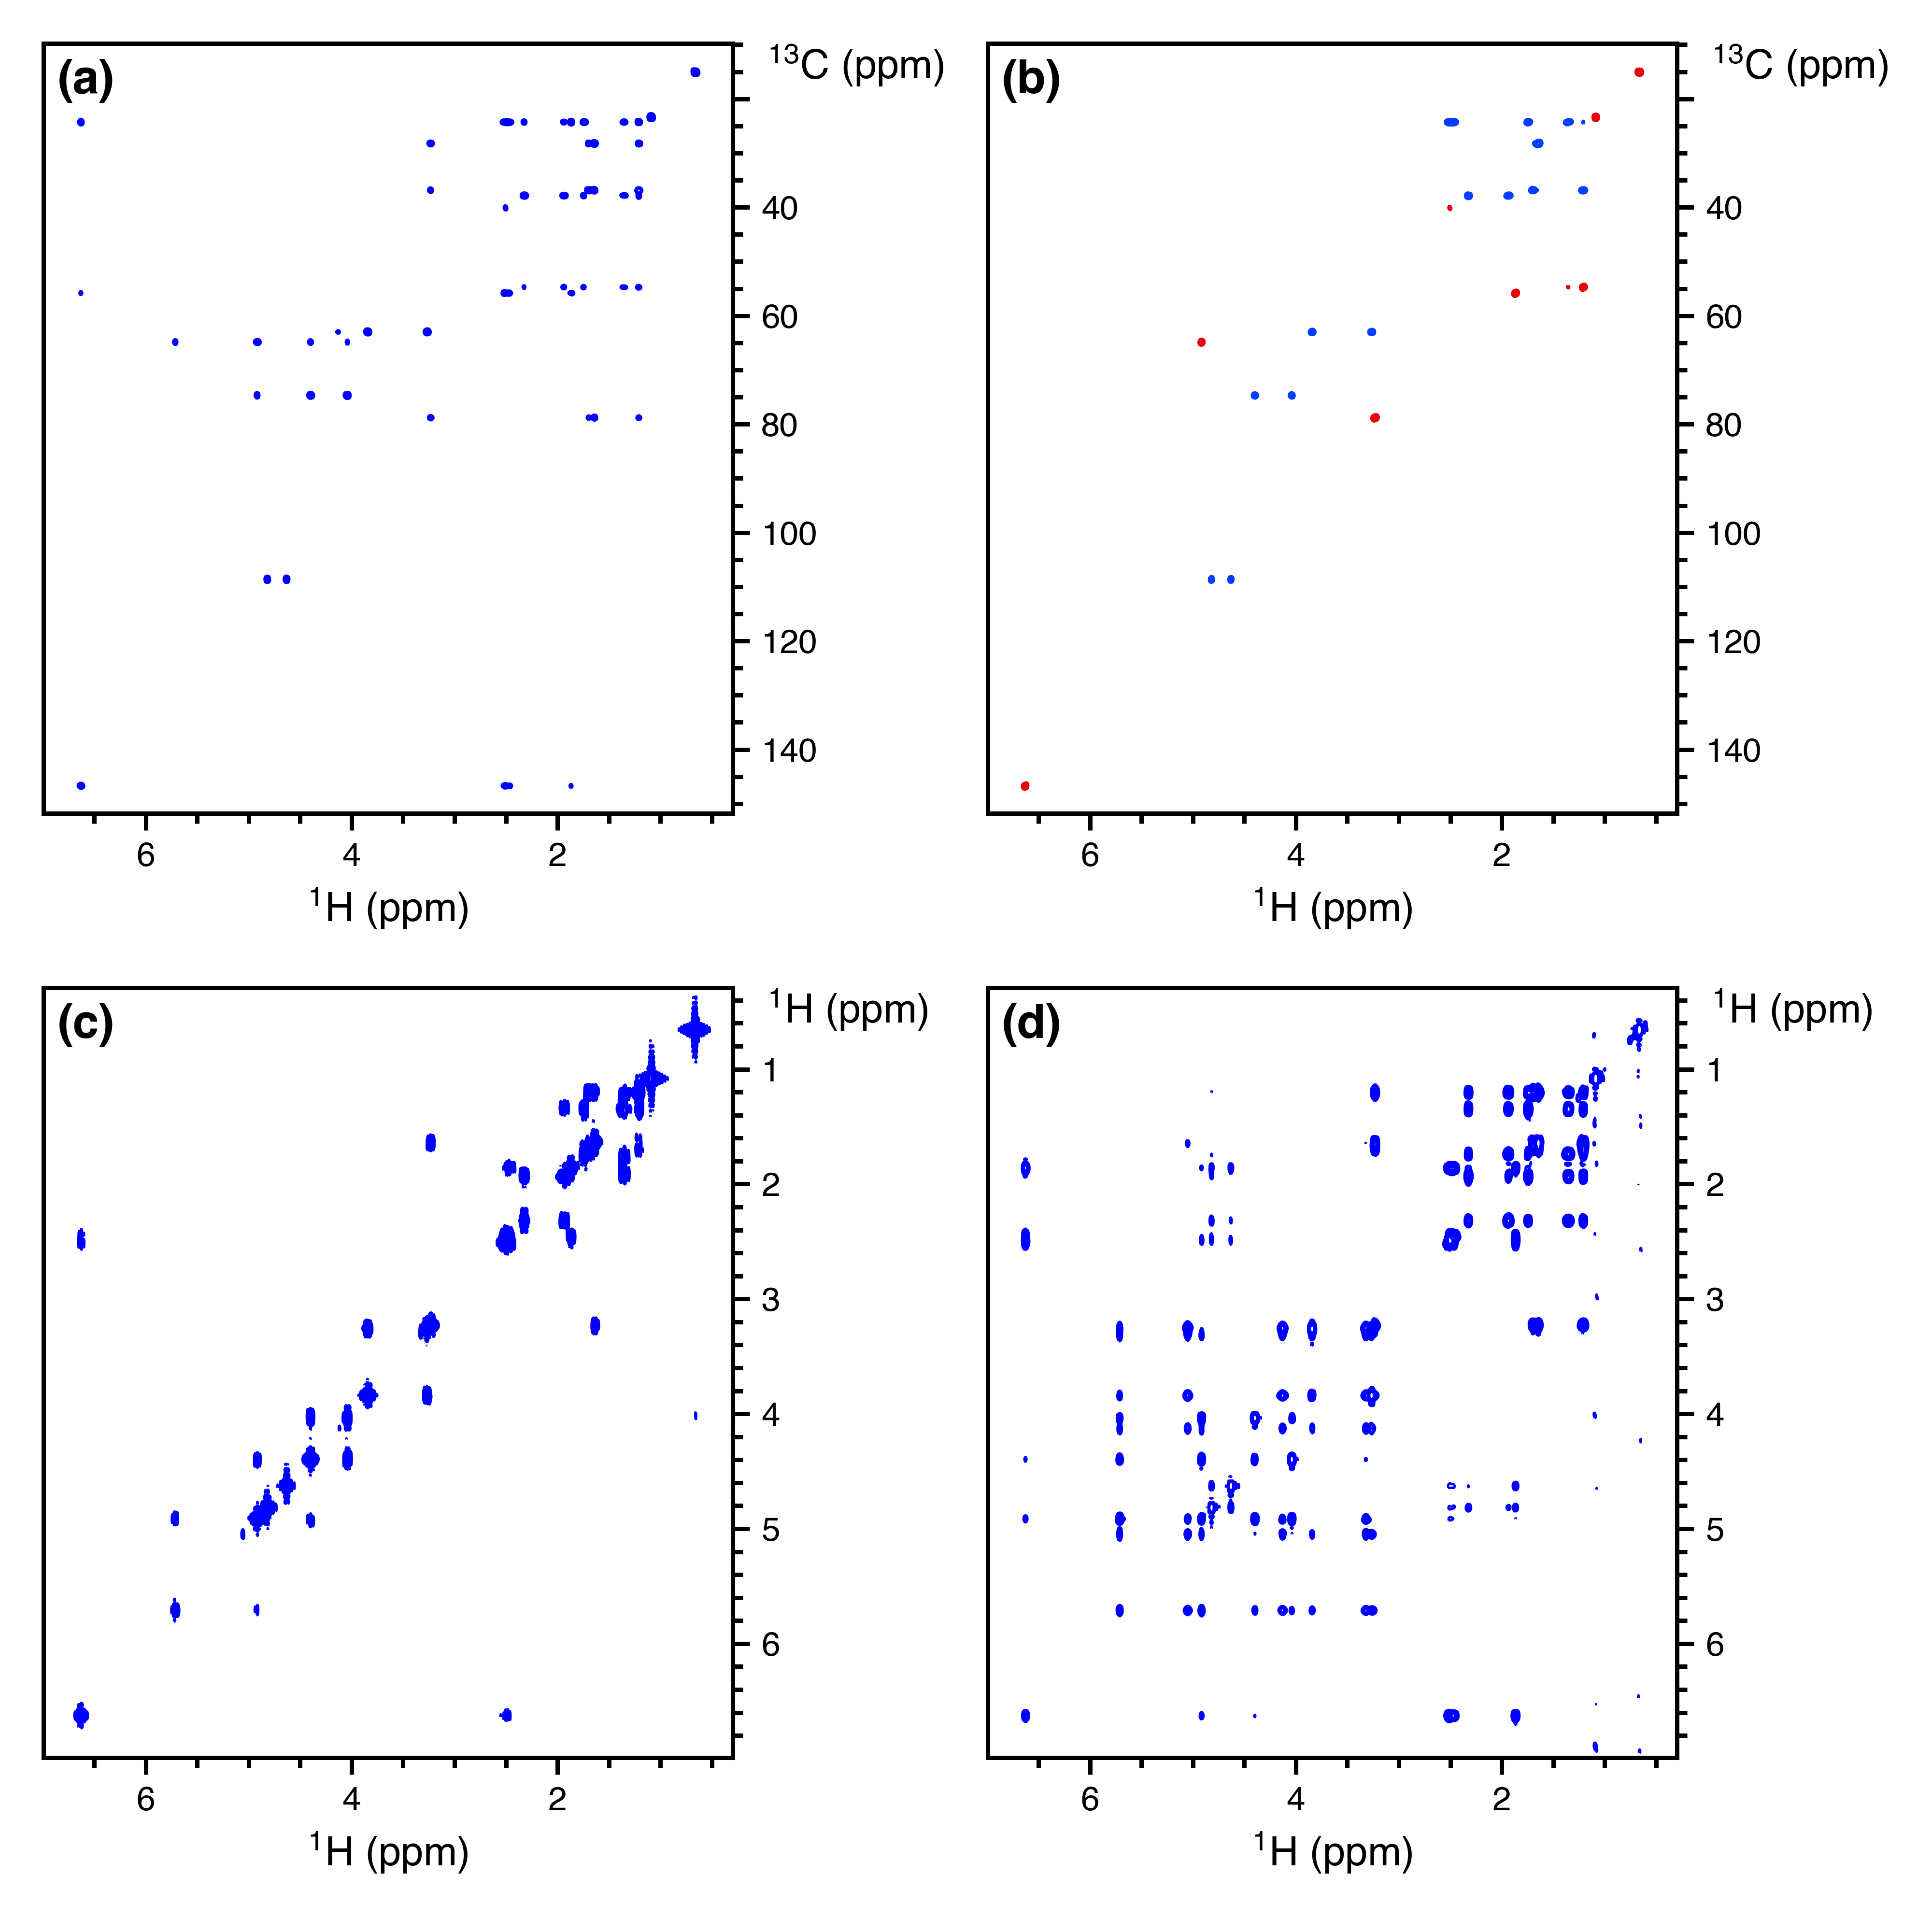
\includegraphics[width=0.8\textwidth]{./figures/stspct.png}
    \caption{
        2D spectra acquired using the NOAH-4 \noahfour{St}{Sp}{C}{T} supersequence.
        256 $t_1$ increments were used with 2 scans per increment, leading to a total experiment time of 17 minutes and 32 seconds.
        This represents a $3.25\times$ time saving relative to conventional acquisition of each of the four spectra with the same parameters, which would take a total of 57 minutes and 3 seconds.
        \textbf{(a)} HSQC-TOCSY (\SI{30}{ms} mixing time, $f = 0.9$).
        \textbf{(b)} Multiplicity edited seHSQC.
        \textbf{(c)} COSY.
        \textbf{(d)} TOCSY (\SI{60}{ms} mixing time).
        \andro{}
    }
    \label{fig:stspct}
\end{figure}

\begin{figure}
    \centering
    % figures/stspct_nus.py
    
\includegraphics{./figures/andro.png}\phantom{aaaaaa}
    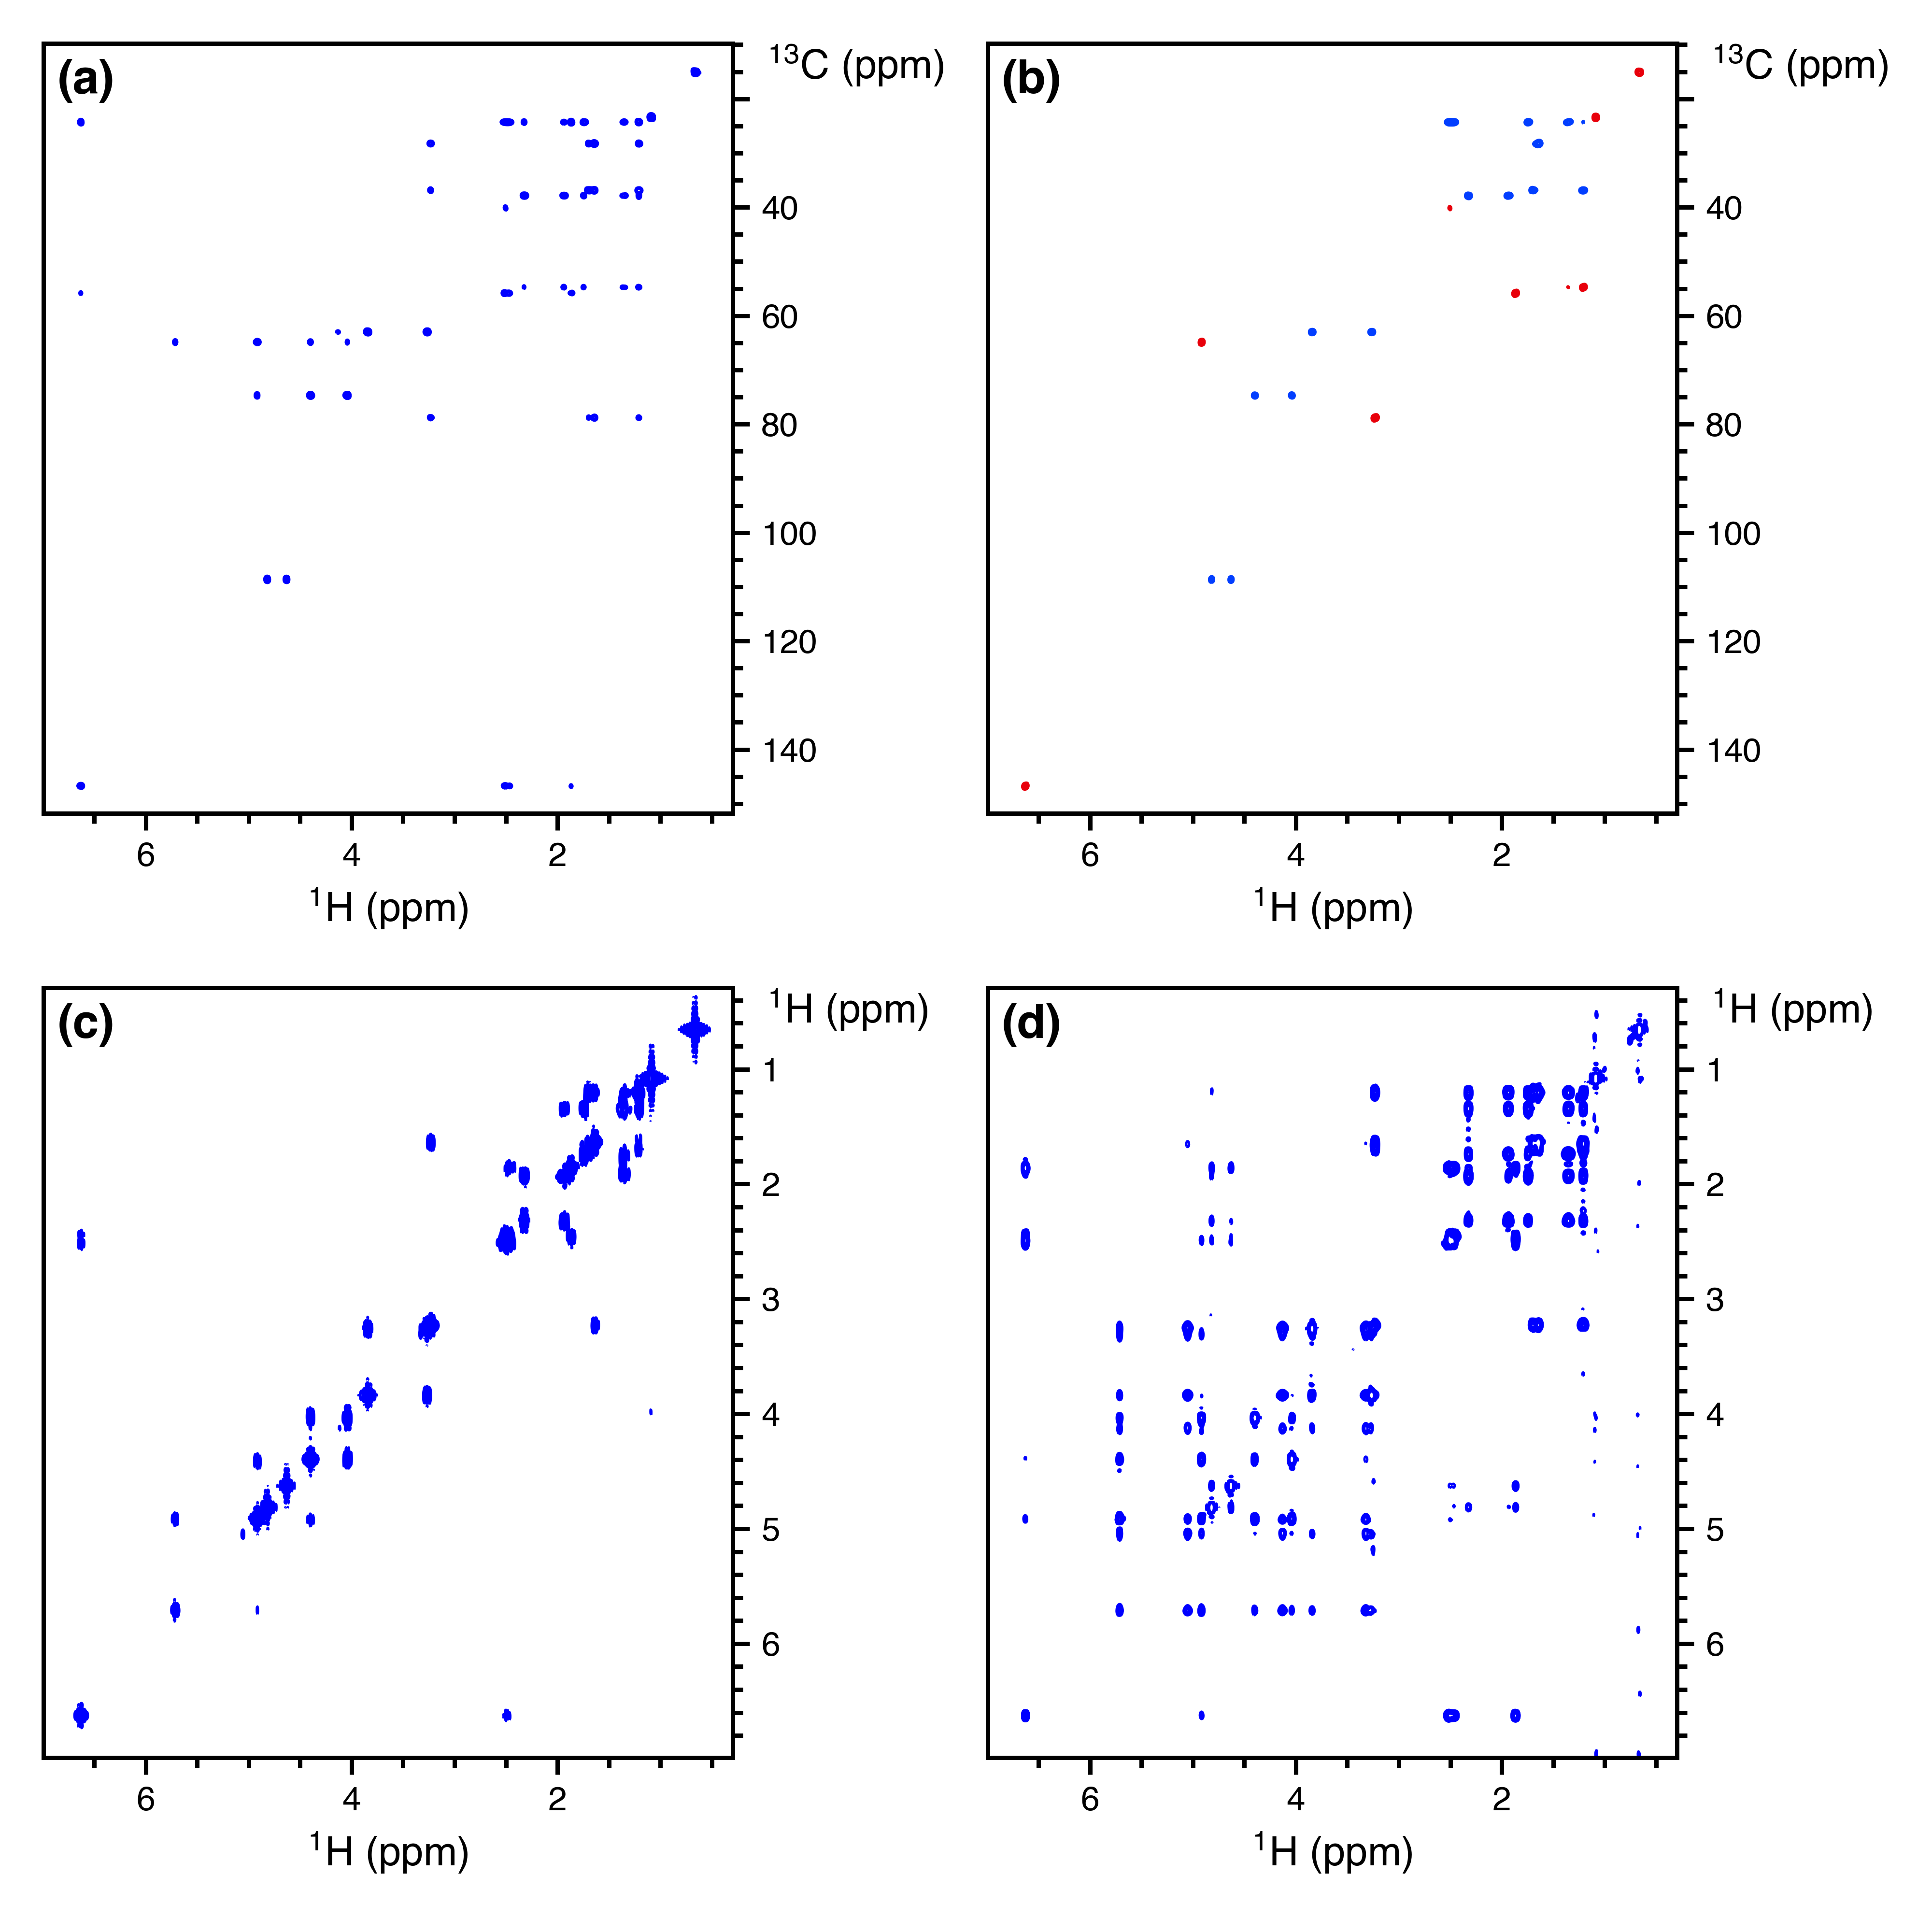
\includegraphics[width=0.8\textwidth]{./figures/stspct_nus.png}
    \caption{
        2D spectra acquired using the NOAH-4 \noahfour{St}{Sp}{C}{T} supersequence with 50\% non-uniform sampling for all modules.
        All other parameters are the same as in \figref{stspct}.
        The experimental time was 9 minutes and 1 second.
        \textbf{(a)} HSQC-TOCSY (\SI{30}{ms} mixing time, $f = 0.9$).
        \textbf{(b)} Multiplicity edited seHSQC.
        \textbf{(c)} COSY.
        \textbf{(d)} TOCSY (\SI{60}{ms} mixing time).
        \andro{}
    }
    \label{fig:stspct_nus}
\end{figure}

\begin{figure}
    \centering
    % figures/bspnspcqf.py
    
\includegraphics{./figures/zolmi.png}\phantom{aaaaaa}

    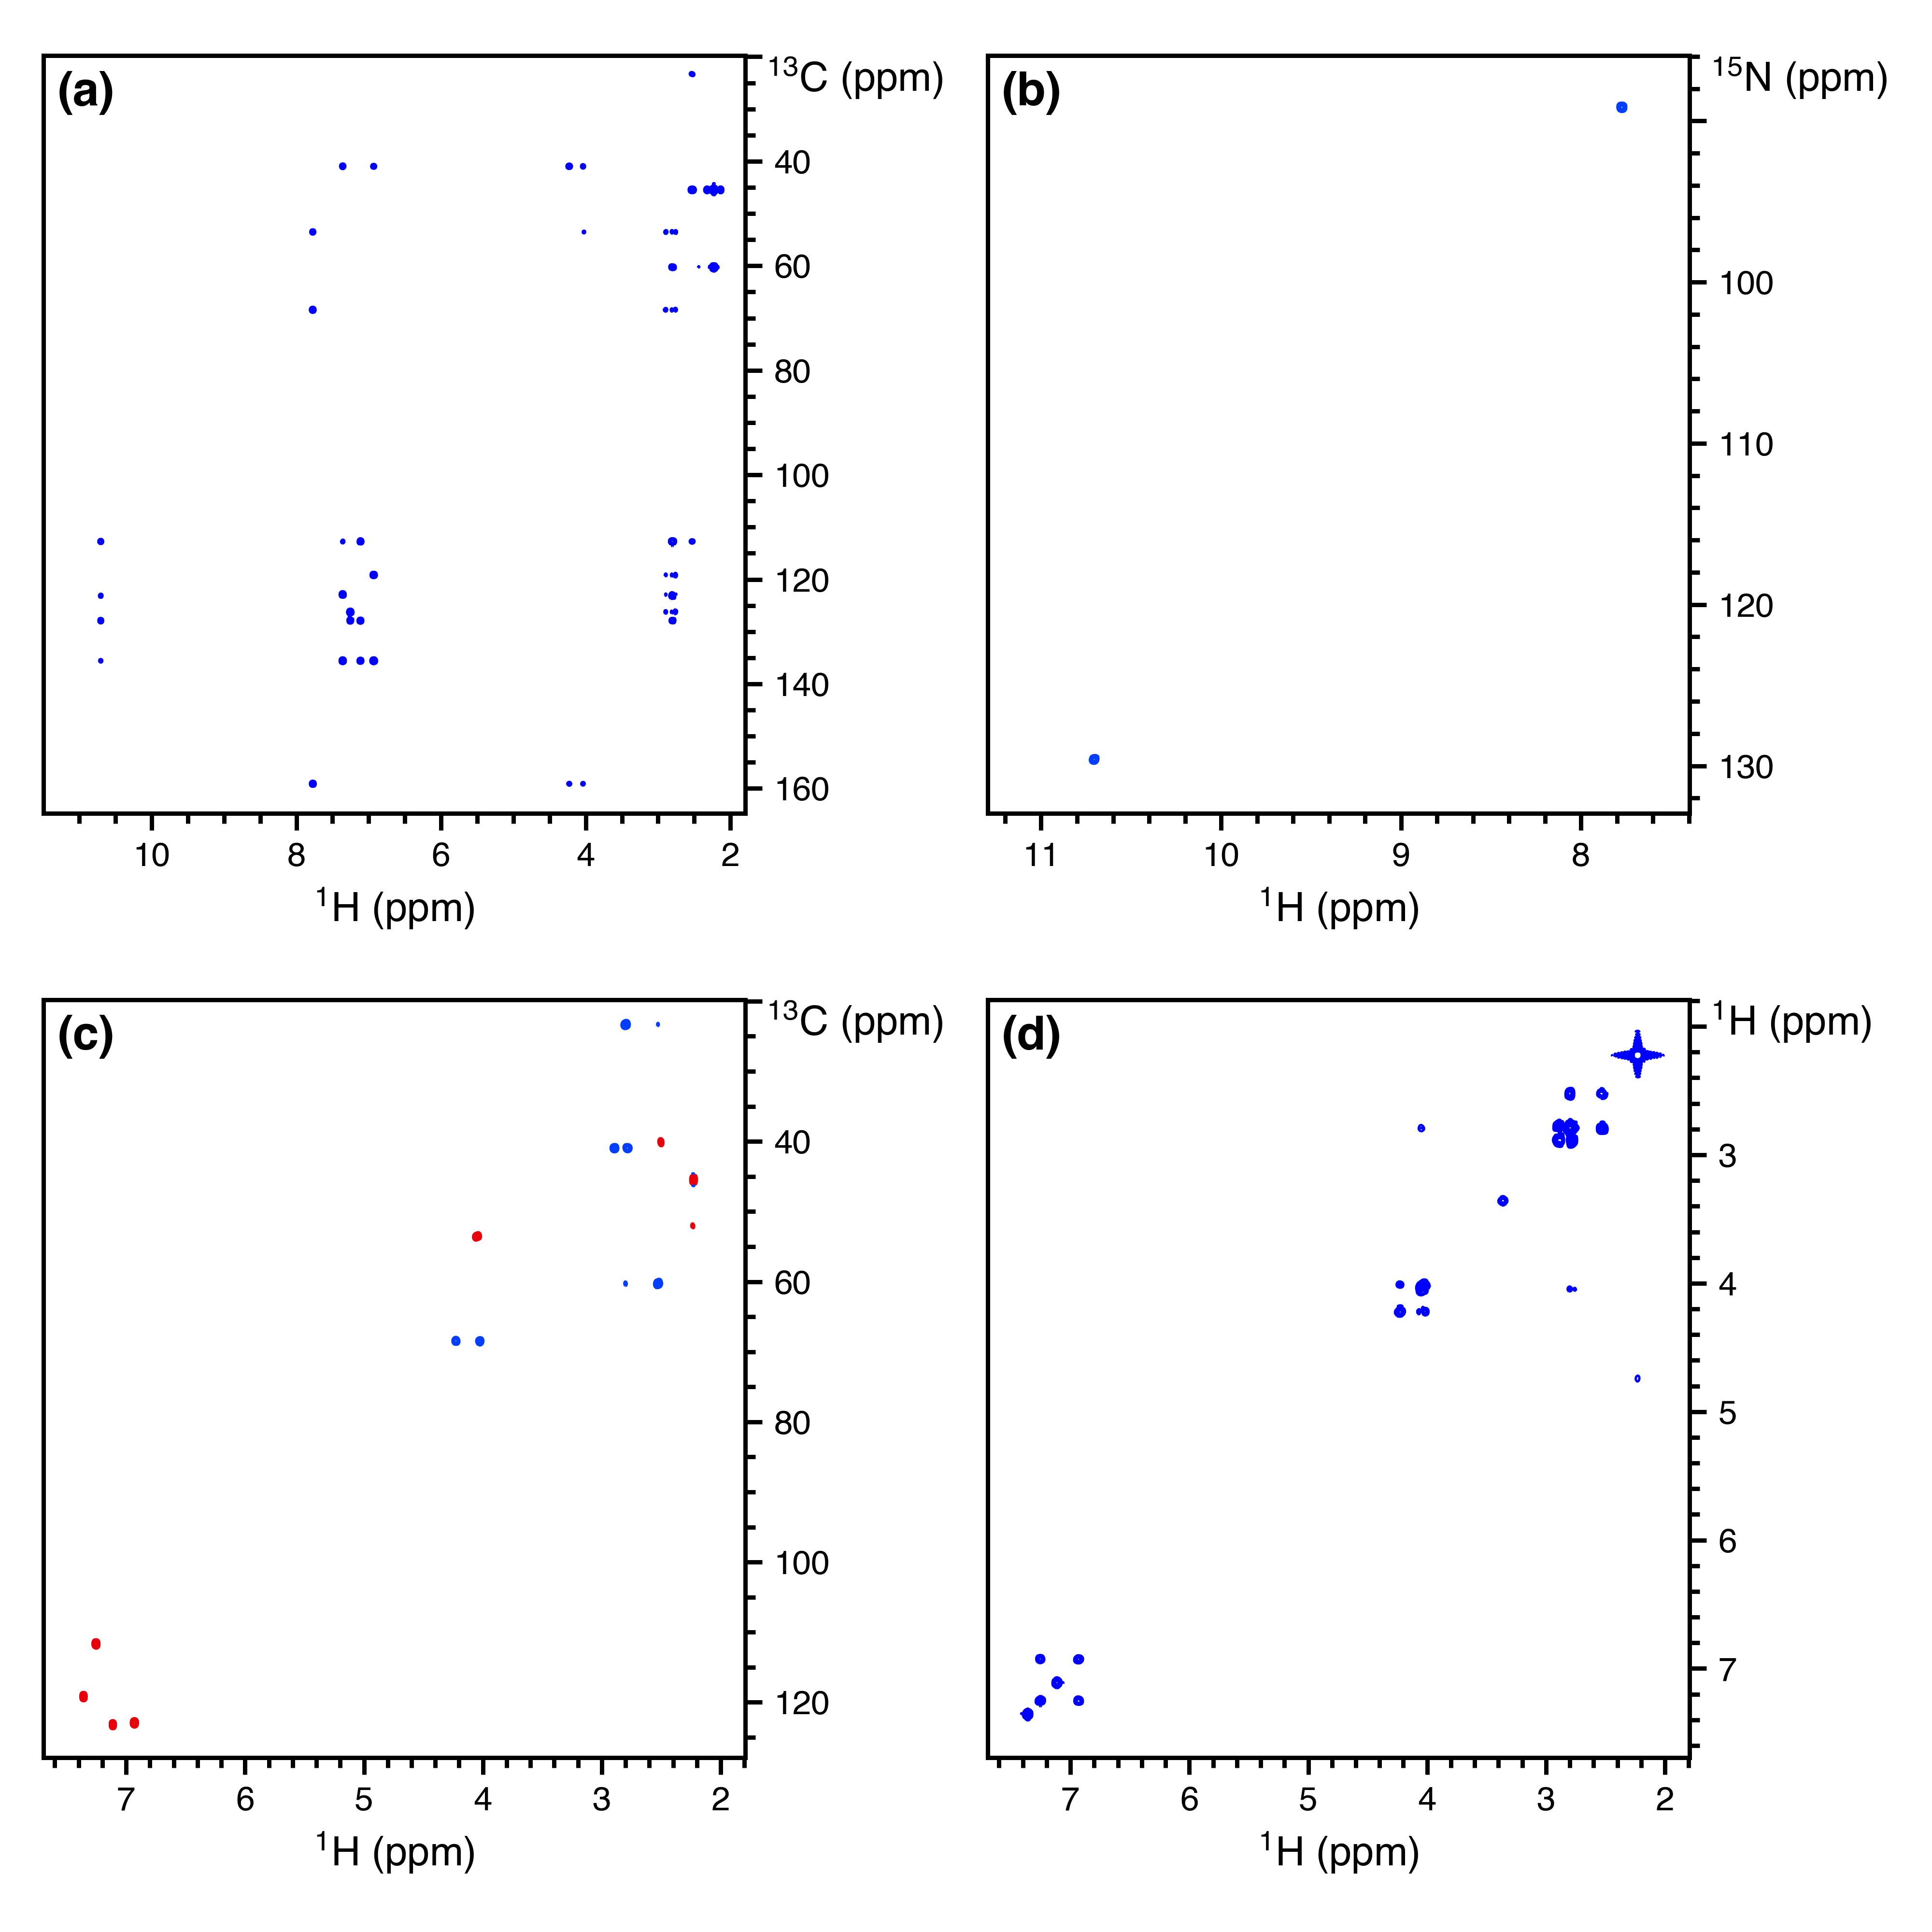
\includegraphics[width=0.8\textwidth]{./figures/bspnspcqf.png}
    \caption{
        2D spectra acquired using the NOAH-4 \noahfour{B}{Spn}{Sp}{Cqf} supersequence.
        256 $t_1$ increments were used with 2 scans per increment, leading to a total experiment time of 17 minutes and 32 seconds.
        This represents a $3.22\times$ time saving relative to conventional acquisition of each of the four spectra with the same parameters, which would take a total of 56 minutes and 28 seconds.
        \textbf{(a)} HMBC.
        \textbf{(b)} \nitrogen{} seHSQC with $k = 4$, linear projected to 512 complex points.
        \textbf{(c)} Multiplicity edited \carbon{} seHSQC.
        \textbf{(d)} Magnitude-mode COSY (Bruker \texttt{qf} mode).
        \zolmi{}
    }
    \label{fig:bspnspcqf}
\end{figure}

\section{Pulse programmes}

\begin{itemize}
    \item SCc
    \item SpCc
    \item MSpCc
    \item SnSpCc
    \item SpnSpCc
    \item SSCc
    \item SSpCc
    \item StSCc
    \item StSpCc
    \item StSpCT
    \item BSpnSpCqf
\end{itemize}

\section{Processing scripts}

We basically need everything, including the new version of NUS.


\end{document}
